% \iffalse meta-comment
%
% Copyright (C) 2005-2014 by Ruini Xue <xueruini@gmail.com>
%
% This file may be distributed and/or modified under the
% conditions of the LaTeX Project Public License, either version 1.3a
% of this license or (at your option) any later version.
% The latest version of this license is in:
%
% http://www.latex-project.org/lppl.txt
%
% and version 1.3a or later is part of all distributions of LaTeX
% version 2004/10/01 or later.
%
% $Id$
%
% \fi
%
% \CheckSum{2472}
% \CharacterTable
%  {Upper-case    \A\B\C\D\E\F\G\H\I\J\K\L\M\N\O\P\Q\R\S\T\U\V\W\X\Y\Z
%   Lower-case    \a\b\c\d\e\f\g\h\i\j\k\l\m\n\o\p\q\r\s\t\u\v\w\x\y\z
%   Digits        \0\1\2\3\4\5\6\7\8\9
%   Exclamation   \!     Double quote  \"     Hash (number) \#
%   Dollar        \$     Percent       \%     Ampersand     \&
%   Acute accent  \'     Left paren    \(     Right paren   \)
%   Asterisk      \*     Plus          \+     Comma         \,
%   Minus         \-     Point         \.     Solidus       \/
%   Colon         \:     Semicolon     \;     Less than     \<
%   Equals        \=     Greater than  \>     Question mark \?
%   Commercial at \@     Left bracket  \[     Backslash     \\
%   Right bracket \]     Circumflex    \^     Underscore    \_
%   Grave accent  \`     Left brace    \{     Vertical bar  \|
%   Right brace   \}     Tilde         \~}
%
% \iffalse
%<*driver>
\ProvidesFile{thuthesis.dtx}[2014/12/09 4.8.1 Tsinghua University Thesis Template]
\documentclass[10pt]{ltxdoc}
\usepackage{dtx-style}
\EnableCrossrefs
\CodelineIndex
\RecordChanges
%\OnlyDescription
\begin{document}
  \DocInput{\jobname.dtx}
\end{document}
%</driver>
% \fi
%
% \GetFileInfo{\jobname.dtx}
%
% \changes{v1.0-}{2005/07/06}{Please refer to ``Bao--Pan'' version.}
% \changes{v1.1}{2005/11/03}{Initial version, migrate from the old ``Bao--Pan''
% version. Make the template a class instead of package.}
% \changes{v1.2}{2005/11/04}{Remove \pkg{fancyref}; Remove \pkg{ucite} and implement
% \cs{onlinecite}; use package \pkg{arial} or \pkg{helvet} selectively.}
% \changes{v1.3}{2005/11/14}{Replace \pkg{subfigure} with \pkg{subfig}, replace \pkg{caption2}
% with \pkg{caption}, add details about using figure are in the example.}
% \changes{v1.4rc1}{2005/11/20}{I do not know why \cs{thu@authorizationaddon} does not work
% now for v1.3, while it's fine in v1.2. Temporarily, I remove the directive
% :(. There might be better solution. Other changes: add \textsf{config} option to
% subfig to be compatible with subfigure. add \pkg{courier} package for tt font.}
% \changes{v1.4}{2005/12/05}{Fix the problem of \textbf{chinese}, which is
% because both CJK and everysel redefine the \cs{selectfont}. So, a not so good
% workaround is merge them up. Add \file{shuji} example. Add \cs{pozhehao} command.}
% \changes{v2.1}{2006/02/27}{Add support to bachelor thesis.}
% \changes{v2.1}{2006/03/01}{Remove \pkg{fancyhdr} and \pkg{geometry}.}
% \changes{v2.1}{2006/03/01}{Redefine footnote marks.}
% \changes{v2.1}{2006/03/01}{Replace \file{thubib.bst} with \file{chinesebst.bst}.}
% \changes{v2.1}{2006/03/02}{Merge the modification of \pkg{ntheorem}.}
% \changes{v2.1}{2006/03/02}{Remove \pkg{footmisc} and refine the document.}
% \changes{v2.1}{2006/03/03}{Work very hard on the document.}
% \changes{v2.1}{2006/03/03}{Add \cs{checklab} code to reduce ``unresolved labels'' warning}
% \changes{v2.2}{2006/03/26}{Adjust margins. How bad it is to simulate MS WORD!.}
% \changes{v2.2}{2006/03/26}{Add bachelor training overview details supporting.}
% \changes{v2.2}{2006/03/26}{CJK support in preamble.}
% \changes{v2.2}{2006/03/26}{Adjust hyperref to avoid boxes around links.}
% \changes{v2.3}{2006/04/07}{Fix a great bug: \cs{PassOptionsToClass} and \cs{LoadClass}
% rather than \cs{PassOptionToPackage} and \cs{LoadPackage}.}
% \changes{v2.3}{2006/04/07}{Reorganize the codes in cover, make the pagestyle more readable.}
% \changes{v2.3}{2006/04/07}{Add gbk2uni into the document.}
% \changes{v2.3}{2006/04/07}{Support \option{openright} and openany.}
% \changes{v2.3}{2006/04/09}{Adjust hypersetup to remove color and box.}
% \changes{v2.3}{2006/04/09}{Adjust margins again.}
% \changes{v2.3}{2006/04/09}{Adjust references formats.}
% \changes{v2.3}{2006/04/09}{Redefine frontmatter and mainmatter to fit our case.}
% \changes{v2.3}{2006/04/09}{Add assumption environment.}
% \changes{v2.3}{2006/04/09}{Change the brace in the cover.}
% \changes{v2.4}{2006/04/14}{Fill more pdf info. with hypersetup.}
% \changes{v2.4}{2006/04/14}{自动隐藏密级为内部时后面的五角星。}
% \changes{v2.4}{2006/04/14}{增加“注释 (Remark)”环境。}
% \changes{v2.4}{2006/04/14}{压缩 item 之间的距离。}
% \changes{v2.4}{2006/04/14}{thubib.bst 文献标题取消自动小写。}
% \changes{v2.4}{2006/04/14}{中文参考文献取消 In: Proceedings。}
% \changes{v2.4}{2006/04/14}{英文文参考文献调整 In: editor, Proceedings。}
% \changes{v2.4}{2006/04/14}{参考文献为学位论文时,加方括号,作者后面为实心点。}
% \changes{v2.4}{2006/04/14}{中文参考文献作者超过三个加等。}
% \changes{v2.4}{2006/04/14}{中文参考文献需要在 bib 中指定 |lang="chinese"|。}
% \changes{v2.4}{2006/04/14}{学位论文不在需要 type 字段。}
% \changes{v2.4}{2006/04/14}{为摘要等条目增加书签。}
% \changes{v2.4}{2006/04/14}{章节的编号用黑体,也就是自动打开 \option{arialtitle} 选项。}
% \changes{v2.4.1}{2006/04/17}{2.4 忘了把关键词的 tabular 改成 thu@tabular。}
% \changes{v2.4.1}{2006/04/17}{参考文献最后一个作者前是逗号而不是 and。}
% \changes{v2.4.2}{2006/04/18}{去掉参考文献第二个作者后面烦人的逗号。}
% \changes{v2.5}{2006/05/19}{对本科论文进行大幅度的重写,因为教务处修改了格式要求。}
% \changes{v2.5}{2006/05/19}{重新整理代码,使其布局更易读。}
% \changes{v2.5.1}{2006/05/24}{根据教务处的新要求调整附录部分。}
% \changes{v2.5.1}{2006/05/25}{参考文献中杂志文章如果没有卷号,那么页码直接跟在
% 年份后面,并用句点分割。在 \file{thubib.bst} 中增加 output.year 函数。}
% \changes{v2.6.1}{2006/06/16}{取消 \file{thubib.bst} 中 inbook 类 volume 后的页码。}
% \changes{v4.5}{2008/01/04}{彻底转向 UTF-8,并支持 xelatex。}
% \changes{v4.6}{2011/04/27}{增加博士后文档部分。}
% \changes{v4.6}{2011/10/22}{使用手册更新。}
% \changes{v4.7}{2012/06/12}{去掉 \pkg{hypernat} 依赖,\pkg{hyperref} 和 \pkg{natbib} 可以很好配合了。}
% \changes{v4.8}{2014/11/25}{好几年累积的一些更新,最重要的是切换到 \pkg{ctex}。}
%
% \DoNotIndex{\begin,\end,\begingroup,\endgroup}
% \DoNotIndex{\ifx,\ifdim,\ifnum,\ifcase,\else,\or,\fi}
% \DoNotIndex{\let,\def,\xdef,\newcommand,\renewcommand}
% \DoNotIndex{\expandafter,\csname,\endcsname,\relax,\protect}
% \DoNotIndex{\Huge,\huge,\LARGE,\Large,\large,\normalsize}
% \DoNotIndex{\small,\footnotesize,\scriptsize,\tiny}
% \DoNotIndex{\normalfont,\bfseries,\slshape,\interlinepenalty}
% \DoNotIndex{\hfil,\par,\hskip,\vskip,\vspace,\quad}
% \DoNotIndex{\centering,\raggedright}
% \DoNotIndex{\c@secnumdepth,\@startsection,\@setfontsize}
% \DoNotIndex{\ ,\@plus,\@minus,\p@,\z@,\@m,\@M,\@ne,\m@ne}
% \DoNotIndex{\@@par,\DeclareOperation,\RequirePackage,\LoadClass}
% \DoNotIndex{\AtBeginDocument,\AtEndDocument}
%
% \IndexPrologue{\section*{索引}%
%    \addcontentsline{toc}{section}{索~~~~引}}
% \GlossaryPrologue{\section*{修改记录}%
%    \addcontentsline{toc}{section}{修改记录}}
%
% \renewcommand{\abstractname}{摘~~要}
% \renewcommand{\contentsname}{目~~录}
%
%
% \title{\thuthesis:清华大学学位论文模板\thanks{Tsinghua University \LaTeX{} Thesis Template.}}
% \author{{\fangsong 薛瑞尼\thanks{LittleLeo@newsmth}}\\[5pt]{\fangsong 清华大学
% 计算机系高性能所\thanks{目前于电子科技大学工作。}}\\[5pt] \texttt{xueruini@gmail.com}}
% \date{v\fileversion\ (\filedate)}
% \maketitle\thispagestyle{empty}
%
%
% \begin{abstract}\noindent
%   此宏包旨在建立一个简单易用的清华大学学位论文模板,包括本科综合论文训练、硕士
%   论文、博士论文以及博士后出站报告。
% \end{abstract}
%
% \vskip2cm
% \def\abstractname{免责声明}
% \begin{abstract}
% \noindent
% \begin{enumerate}
% \item 本模板的发布遵守 \LaTeX{} Project Public License,使用前请认真阅读协议内
%   容。
% \item 本模板为作者根据清华大学教务处颁发的《综合论文训练写作指南》,清华大学研
%   究生院颁发的《研究生学位论文写作指南》,清华大学《编写“清华大学博士后研究报
%   告”参考意见》编写而成,旨在供清华大学毕业生撰写学位论文使用。
% \item 清华大学教务处和研究生院只提供毕业论文写作指南,不提供官方模板,也不会授
%   权第三方模板为官方模板,所以此模板仅为写作指南的参考实现,不保证格式审查老师
%   不提意见。任何由于使用本模板而引起的论文格式审查问题均与本模板作者无关。
% \item 任何个人或组织以本模板为基础进行修改、扩展而生成的新的专用模板,请严格遵
%   守 \LaTeX{} Project Public License 协议。由于违犯协议而引起的任何纠纷争端均与
%   本模板作者无关。
% \end{enumerate}
% \end{abstract}
%
%
% \clearpage
% \begin{multicols}{2}[
%   \section*{\contentsname}
%   \setlength{\columnseprule}{.4pt}
%   \setlength{\columnsep}{18pt}]
%   \tableofcontents
% \end{multicols}
%
% \clearpage
% \pagenumbering{arabic}
% \pagestyle{headings}
% \section{模板介绍}
% \thuthesis\ (\textbf{T}sing\textbf{hu}a \textbf{Thesis}) 是为了帮助清华大学毕业
% 生撰写毕业论文而编写的 \LaTeX{} 论文模板。
%
% 本文档将尽量完整的介绍模板的使用方法,如有不清楚之处可以参考示例文档或者根据
% 第~\ref{sec:howtoask}节说明提问,有兴趣者都可以参与完善此手册,也非常欢迎对代
% 码的贡献。
%
% {\color{blue}\fangsong 模板的作用在于减少论文写作过程中格式调整的时间,前提是遵
% 守模板的用法,否则即便用了 \thuthesis{} 也难以保证输出的论文符合学校规范。}
%
%
% \section{安装}
% \label{sec:installation}
%
% \subsection{下载}
% \thuthesis{} 相关链接:
% \begin{itemize}
% \item 主页:\href{https://github.com/xueruini/thuthesis}{GitHub}
% \item 下载:\href{http://www.ctan.org/pkg/thuthesis}{CTAN}
% \end{itemize}
% 除此之外,不再维护任何镜像。
%
%
% \subsection{模板的组成部分}
% 下表列出了 \thuthesis{} 的主要文件及其功能介绍:
%
% \begin{center}
%   \begin{longtable}{l|p{8cm}}
% \hline
% {\heiti 文件(夹)} & {\heiti 功能描述}\\\hline\hline
% \endfirsthead
% \hline
% {\heiti 文件(夹)} & {\heiti 功能描述}\\\hline\hline
% \endhead
% \endfoot
% \endlastfoot
% thuthesis.ins & 模板驱动文件 \\
% thuthesis.dtx & 模板文档代码的混合文件\\
% thuthesis.cls & 模板类文件\\
% thuthesis.cfg & 模板配置文件\\
% thufonts.def & 中文字体配置文件\\
% thubib.bst & 参考文献样式文件\\\hline
% main.tex & 示例文档主文件\\
% shuji.tex & 书脊示例文档\\
% ref/ & 示例文档参考文献目录\\
% data/ & 示例文档章节具体内容\\
% figures/ & 示例文档图片路径\\
% thutils.sty & 为示例文档加载其它宏包\\\hline
% Makefile & self-explanation\\
% zhfonts.py & 生成中文字体配置文件\\
% README.md & self-explanation\\
% \textbf{thuthesis.pdf} & 用户手册(本文档)\\\hline
%   \end{longtable}
% \end{center}
% 几点说明:
% \begin{itemize}
% \item \file{thuthesis.cls} 和 \file{thuthesis.cfg} 可以由 \file{thuthesis.ins}
%   和 \file{thuthesis.dtx} 生成,但为了降低新手用户的使用难度,故
%   将 \file{thuthesis.cls} 和 \file{thuthesis.cfg} 文件一起发布。
% \item 使用前阅读文档:\file{thuthesis.pdf}.
% \end{itemize}
% 
% \subsection{准备工作}
% \label{sec:prepare}
% 本模板用到的主要宏包包括:
%
% \begin{center}
% \begin{minipage}{1.0\linewidth}\centering
% \begin{tabular}{*{6}{l}}\hline
%   \pkg{ifxetex} & \pkg{xunicode} & \pkg{CJK}        & \pkg{xeCJK}    & \pkg{CJKpunct} & \pkg{ctex} \\
%   \pkg{array}   & \pkg{booktabs} & \pkg{longtable}  &  \pkg{amsmath} & \pkg{amssymb}  & \pkg{ntheorem} \\
%   \pkg{indentfirst} & \pkg{paralist} & \pkg{txfonts} & \pkg{natbib} & \pkg{hyperref}  & \pkg{graphicx} \\
%   \pkg{subcaption}  &  \pkg{caption} & \pkg{thubib.bst} & & & \\\hline
% \end{tabular}
% \end{minipage}
% \end{center}
%
% 这些包在常见的 \TeX{} 系统中都有,如果没有请到 \url{www.ctan.org} 下载。
%
%
% \subsection{开始安装}
% \label{sec:install}
%
% \subsubsection{生成模板}
% \label{sec:generate-cls}
% {\heiti 说明:默认的发行包中已经包含了所有文件,可以直接使用。如果对如何生成模
% 板文件以及模板文档不感兴趣,请跳过本小节。}
%
% 模板解压缩后生成文件夹 \file{thuthesis-VERSION}\footnote{VERSION 为版本号。},
% 其中包括:模板源文件(\file{thuthesis.ins} 和 \file{thuthesis.dtx}),参考文献
% 样式 \file{thubib.bst},示例文档
% (\file{main.tex},\file{shuji.tex},\file{thufonts.def}\footnote{Xe\LaTeX 中文
% 字体配置文件},\file{thutils.sty}\footnote{可能用到的包以及一些命令定义都放在这
% 里,以免 \file{thuthesis.cls} 过分臃
% 肿。},\file{data/} 和 \file{figures/} 和 \file{ref/})。在使用之前需要先生成模
% 板文件和配置文件(具体命令细节请参考 \file{README.md} 和 \file{Makefile}):
%
% \begin{shell}
% $ cd thuthesis-VERSION
% # 生成 thuthesis.cls 和 thuthesis.cfg
% $ latex thuthesis.ins
%
% # 下面的命令用来生成用户手册,可以不执行
% $ xelatex thuthesis.dtx
% $ makeindex -s gind.ist -o thuthesis.ind thuthesis.idx
% $ makeindex -s gglo.ist -o thuthesis.gls thuthesis.glo
% $ xelatex thuthesis.dtx
% $ xelatex thuthesis.dtx  % 生成说明文档 thuthesis.pdf
% \end{shell}
%
%
% \subsubsection{dvi$\rightarrow$ps$\rightarrow$pdf}
% \label{sec:dvipspdf}
% 很多用户对 \LaTeX{} 命令执行的次数不太清楚,一个基本的原则是多次运行 \LaTeX{}命
% 令直至不再出现警告。下面给出生成示例文档的详细过程(\# 开头的行为注释),首先来
% 看经典的 \texttt{dvi$\rightarrow$ps$\rightarrow$pdf} 方式:
% \begin{shell}
% # 1. 发现里面的引用关系,文件后缀 .tex 可以省略
% $ latex main
%
% # 2. 编译参考文件源文件,生成 bbl 文件
% $ bibtex main
%
% # 3. 下面解决引用
% $ latex main
% # 如果是 GBK 编码,此处运行:
% # $ gbk2uni main  # 防止书签乱码
% $ latex main   # 此时生成完整的 dvi 文件
%
% # 4. 生成 ps
% $ dvips main.dvi
%
% # 5. 生成 pdf
% $ ps2pdf main.ps
% \end{shell}
%
% 模板已经把纸型信息写入目标文件,这样执行 \texttt{dvips} 时就可以避免由于遗忘
%  \texttt{-ta4} 参数而导致输出不合格的文件(因为 \texttt{dvips} 默认使用
%  letter 纸型)。
%
% \subsubsection{dvipdfm(x)}
% \label{sec:dvipdfmx}
% 如果使用 \texttt{dvipdfm(x)},那么在生成完整的 dvi 文件之后(参见上面的例子),
% 可以直接得到 pdf:
% \begin{shell}%
% $ dvipdfm  main.dvi
% # 或者
% $ dvipdfmx  main.dvi
% \end{shell}
%
% \subsubsection{pdflatex}
% \label{sec:pdflatex}
% 如果使用 PDF\LaTeX,按照第~\ref{sec:dvipspdf} 节的顺序执行到第 3 步即可,不再经
% 过中间转换。
%
% 需要注意的是 PDF\LaTeX\ 不能处理常见的 EPS 图形,需要先用 epstopdf 将其转化
% 成 PDF。不过 PDF\LaTeX\ 增加了对 png,jpg 等标量图形的支持,比较方便。
%
% \subsubsection{xelatex}
% \label{sec:xelatex}
% Xe\TeX 最大的优势就是不再需要繁琐的字体配置。\thuthesis{} 通过 \pkg{xeCJK} 来控
% 制中文字体和标点压缩。模板里默认用的是中易的四款免费字体(宋,黑,楷,仿宋),
% 用户可以根据自己的实际情况自行替换。另外,本科论文封面要用到隶书,请用户自行修
% 改。字体配置参考第~\ref{sec:font-config} 节。
%
% Xe\LaTeX\ 的使用步骤同 PDF\LaTeX。
%
%
% \subsubsection{自动化过程}
% \label{sec:automation}
% 上面的例子只是给出一般情况下的使用方法。虽然命令很简单,但是每次都输入的话还是
% 非常罗嗦的,所以 \thuthesis{} 还提供了一些自动处理的文件。
%
% 我们提供了一个简单的 \file{Makefile}:
% \begin{shell}
% $ make clean
% $ make cls       # 生成 thuthesis.cls 和 thuthesis.cfg
% $ make doc       # 生成说明文档 thuthesis.pdf
% $ make thesis    # 生成示例文档 main.pdf
% $ make shuji     # 生成书脊 shuji.pdf
% \end{shell}
%
% \file{Makefile} 默认采用 Xe\LaTeX\ 编译,可以根据自己的需要修
% 改 \file{Makefile} 开头的参数设置或通过命令行传递参数(请参看 \file{README.md})。
%
%
% \subsection{升级}
% \label{sec:updgrade}
% \thuthesis{} 升级非常简单,可以通过 TeX 发行版的包管理工具自动更新发行版,也可
% 以下载最新的开发版,
% 将 \file{thuthesis.ins},\file{thuthesis.dtx} 和 \file{thubib.bst} 拷贝至工作目
% 录覆盖相应的文件,然后运行:
% \begin{shell}
% $ latex thuthesis.ins
% \end{shell}
%
% 生成新的类文件和配置文件即可。也可以直接拷
% 贝 \file{thuthesis.cls},\file{thuthesis.cfg}和 \file{thubib.bst},免去上面命令
% 的执行。
%
%
% \section{使用说明}
% \label{sec:usage}
% 本手册假定用户已经能处理一般的 \LaTeX{} 文档,并对 \BibTeX{} 有一定了解。如果
% 从来没有接触过 \TeX 和 \LaTeX,建议先学习相关的基础知识。磨刀不误砍柴工!
%
% \subsection{关于提问}
% \label{sec:howtoask}
% 按照优先级推荐提问的位置如下:
%
% \begin{itemize}
% \item \href{http://github.com/xueruini/thuthesis/issues}{Github Issues}
% \item \href{http://www.newsmth.net/nForum/#!board/TeX}{Tex@newsmth}
% \item \href{http://groups.google.com/group/thuthesis}{ThuThesis@Google Groups}
% \end{itemize}
%
% \subsection{\thuthesis{} 使用向导}
% \label{sec:userguide}
% 推荐新用户先看网上的《\thuthesis{} 使用向导》幻灯片\footnote{有点老了,不过还是
%   很有帮助的。},那份讲稿比这份文档简练易懂。
%
% \subsection{\thuthesis{} 示例文件}
% \label{sec:userguide1}
% 模板核心文件有四
% 个:\file{thuthesis.cls},\file{thuthesis.cfg},\file{thufonts.def} 和
% \file{thubib.bst},但是如果没有示例文档用户会发现很难下手。所以推荐新用户从模板
% 自带的示例文档入手,里面包括了论文写作用到的所有命令及其使用方法,只需要用自己
% 的内容进行相应替换就可以。对于不清楚的命令可以查阅本手册。下面的例子描述了模板
% 中章节的组织形式,来自于示例文档,具体内容可以参考模板附带
% 的 \file{main.tex} 和 \file{data/}。
%
% \begin{example}
% \documentclass[bachelor,nofonts]{thuthesis}
% %\documentclass[master,adobefonts]{thuthesis}
% %\documentclass[doctor]{thuthesis}
% %\documentclass[%
% %  bachelor|master|doctor|postdoctor, % 必选选项
% %  winfonts|nofonts|adobefonts, % 本科生、Linux 用户使用 XeLaTeX 时必选
% %  secret, % 可选选项
% %  openany|openright, % 可选选项
% %  arialtoc,arialtitle % 可选选项
% %  ]{thuthesis}
% % 当使用 xelatex 编译时,本科生、Linux 用户需要加上 nofonts 选项;
% % 当使用 pdflatex 编译时,adobefonts 选项等效于 winfonts 选项(缺省选项)。
%
% % 所有其它可能用到的包都统一放到这里了,可以根据自己的实际添加或者删除。
% \usepackage{thutils}
%
% % 可以在这里修改配置文件中的定义,导言区可以使用中文。
% % \def\myname{薛瑞尼}
%
% \begin{document}
%
% % 指定图片的搜索目录
% \graphicspath{{figures/}}
%
%
% %%% 封面部分
% \frontmatter
% 
%%% Local Variables:
%%% mode: latex
%%% TeX-master: t
%%% End:

% 中国海洋大学研究生学位论文封面
% 参考:中国海洋大学研究生学位论文书写格式20130307.doc

% 为避免出现错误,下面保留[清华大学学位论文模板原有定义无需修改],
% 请直接跳到后面[中国海洋大学学位论文模板部分请根据自己情况修改]。

%%%%%%%%%%%%%%%%%%%%%%[清华大学学位论文模板原有定义无需修改]%%%%%%%%%%%%%%%%%%%%%%%
\secretlevel{绝密} \secretyear{2100}

\ctitle{清华大学学位论文 \LaTeX\ 模板\\使用示例文档}
% 根据自己的情况选,不用这样复杂
\makeatletter
\ifthu@bachelor\relax\else
  \ifthu@doctor
    \cdegree{工学博士}
  \else
    \ifthu@master
      \cdegree{工学硕士}
    \fi
  \fi
\fi
\makeatother


\cdepartment[计算机]{计算机科学与技术系}
\cmajor{计算机科学与技术}
\cauthor{薛瑞尼} 
\csupervisor{郑纬民教授}
% 如果没有副指导老师或者联合指导老师,把下面两行相应的删除即可。
\cassosupervisor{陈文光教授}
\ccosupervisor{某某某教授}
% 日期自动生成,如果你要自己写就改这个cdate
%\cdate{\CJKdigits{\the\year}年\CJKnumber{\the\month}月}

% 博士后部分
% \cfirstdiscipline{计算机科学与技术}
% \cseconddiscipline{系统结构}
% \postdoctordate{2009年7月——2011年7月}

\etitle{An Introduction to \LaTeX{} Thesis Template of Tsinghua University} 
% 这块比较复杂,需要分情况讨论:
% 1. 学术型硕士
%    \edegree:必须为Master of Arts或Master of Science(注意大小写)
%              “哲学、文学、历史学、法学、教育学、艺术学门类,公共管理学科
%               填写Master of Arts,其它填写Master of Science”
%    \emajor:“获得一级学科授权的学科填写一级学科名称,其它填写二级学科名称”
% 2. 专业型硕士
%    \edegree:“填写专业学位英文名称全称”
%    \emajor:“工程硕士填写工程领域,其它专业学位不填写此项”
% 3. 学术型博士
%    \edegree:Doctor of Philosophy(注意大小写)
%    \emajor:“获得一级学科授权的学科填写一级学科名称,其它填写二级学科名称”
% 4. 专业型博士
%    \edegree:“填写专业学位英文名称全称”
%    \emajor:不填写此项
\edegree{Doctor of Engineering} 
\emajor{Computer Science and Technology} 
\eauthor{Xue Ruini} 
\esupervisor{Professor Zheng Weimin} 
\eassosupervisor{Chen Wenguang} 
% 这个日期也会自动生成,你要改么?
% \edate{December, 2005}

% 定义中英文摘要和关键字
\begin{cabstract}
  论文的摘要是对论文研究内容和成果的高度概括。摘要应对论文所研究的问题及其研究目
  的进行描述,对研究方法和过程进行简单介绍,对研究成果和所得结论进行概括。摘要应
  具有独立性和自明性,其内容应包含与论文全文同等量的主要信息。使读者即使不阅读全
  文,通过摘要就能了解论文的总体内容和主要成果。

  论文摘要的书写应力求精确、简明。切忌写成对论文书写内容进行提要的形式,尤其要避
  免“第 1 章……;第 2 章……;……”这种或类似的陈述方式。

  本文介绍清华大学论文模板 \thuthesis{} 的使用方法。本模板符合学校的本科、硕士、
  博士论文格式要求。

  本文的创新点主要有:
  \begin{itemize}
    \item 用例子来解释模板的使用方法;
    \item 用废话来填充无关紧要的部分;
    \item 一边学习摸索一边编写新代码。
  \end{itemize}

  关键词是为了文献标引工作、用以表示全文主要内容信息的单词或术语。关键词不超过 5
  个,每个关键词中间用分号分隔。(模板作者注:关键词分隔符不用考虑,模板会自动处
  理。英文关键词同理。)
\end{cabstract}

\ckeywords{\TeX, \LaTeX, CJK, 模板, 论文}

\begin{eabstract} 
   An abstract of a dissertation is a summary and extraction of research work
   and contributions. Included in an abstract should be description of research
   topic and research objective, brief introduction to methodology and research
   process, and summarization of conclusion and contributions of the
   research. An abstract should be characterized by independence and clarity and
   carry identical information with the dissertation. It should be such that the
   general idea and major contributions of the dissertation are conveyed without
   reading the dissertation. 

   An abstract should be concise and to the point. It is a misunderstanding to
   make an abstract an outline of the dissertation and words ``the first
   chapter'', ``the second chapter'' and the like should be avoided in the
   abstract.

   Key words are terms used in a dissertation for indexing, reflecting core
   information of the dissertation. An abstract may contain a maximum of 5 key
   words, with semi-colons used in between to separate one another.
\end{eabstract}

\ekeywords{\TeX, \LaTeX, CJK, template, thesis}
%%%%%%%%%%%%%%%%%%%%%%%%%%%%%%%%%%%%%%%%%%%%%%%%%%%%%%%%%%%%%%%%%%%%%%%%%%%%%%%%

%%%%%%%%%%%%%%%%%%[中国海洋大学学位论文模板部分请根据自己情况修改]%%%%%%%%%%%%%%%%%%%
% 中国海洋大学研究生学位论文封面
% 必须填写的内容包括(其他最好不要修改):
%   分类号、密级、UDC
%   论文中文题目、作者中文姓名
%   论文答辩时间
%   封面感谢语
%   论文英文题目
%   中文摘要、中文关键词
%   英文摘要、英文关键词
%
%%%%%[自定义]%%%%%
\newcommand{\fenleihao}{}%分类号
\newcommand{\miji}{}%密级 
                    % 绝密$\bigstar$20年 
                    % 机密$\bigstar$10年
                    % 秘密$\bigstar$5年
\newcommand{\UDC}{}%UDC
\newcommand{\oucctitle}{图像中环结构特征及其应用}%论文中文题目
\ctitle{图像中环结构特征及其应用}%必须修改因为页眉中用到
\cauthor{***}%可以选择修改因为仅在 pdf 文档信息中用到
\cdegree{工学博士}%可以选择修改因为仅在 pdf 文档信息中用到
\ckeywords{环结构特征, 图论, 视网膜图像配准, 扇贝图像识别}%可以选择修改因为仅在 pdf 文档信息中用到
\newcommand{\ouccauthor}{***}%作者中文姓名
%\newcommand{\ouccsupervisor}{姬光荣教授}%作者导师中文姓名
%\newcommand{\ouccdegree}{博\hspace{1em}士}%作者申请学位级别
%\newcommand{\ouccmajor}{海洋信息探测与处理}%作者专业名称
%\newcommand{\ouccdateday}{\CJKdigits{\the\year}年\CJKnumber{\the\month}月\CJKnumber{\the\day}日}
%\newcommand{\ouccdate}{\CJKdigits{\the\year}年\CJKnumber{\the\month}月}
\newcommand{\oucdatedefense}{}%论文答辩时间
%\newcommand{\oucdatedegree}{2009年6月}%学位授予时间
\newcommand{\oucgratitude}{谨以此论文献给我的导师和亲人!}%封面感谢语

\newcommand{\oucetitle}{Cycle strcutural feature in image and its applications}%论文英文题目
%\newcommand{\ouceauthor}{Haiyong Zheng}%作者英文姓名
\newcommand{\oucthesis}{\textsc{OUCThesis}}
%%%%%默认自定义命令%%%%%
% 空下划线定义
\newcommand{\oucblankunderline}[1]{\rule[-2pt]{#1}{.7pt}}
\newcommand{\oucunderline}[2]{\underline{\hskip #1 #2 \hskip#1}}

% 论文封面第一页
%%不需要改动%%
\vspace*{5cm}
{\xiaoer\heiti\oucgratitude

\begin{flushright}
---\hspace*{-2mm}---\hspace*{-2mm}---\hspace*{-2mm}---\hspace*{-2mm}---\hspace*{-2mm}---\hspace*{-2mm}---\hspace*{-2mm}---\hspace*{-2mm}---\hspace*{-2mm}---~\ouccauthor
\end{flushright}
}


\newpage
\mbox{}
\newpage

% 论文封面第二页
%%不需要改动%%
\vspace*{1cm}
\begin{center}
  {\xiaoer\heiti\oucctitle}
\end{center}
\vspace{10.7cm}
{\normalsize\songti
\begin{flushright}
{\renewcommand{\arraystretch}{1.3}
  \begin{tabular}{r@{}l}
    学位论文答辩日期:~ & \oucunderline{1.8em}{\oucdatedefense} \\
    指导教师签字:~ & \oucblankunderline{5cm} \\
    答辩委员会成员签字:~ & \oucblankunderline{5cm} \\
    ~ & \oucblankunderline{5cm} \\
    ~ & \oucblankunderline{5cm} \\
    ~ & \oucblankunderline{5cm} \\
    ~ & \oucblankunderline{5cm} \\
    ~ & \oucblankunderline{5cm} \\
    ~ & \oucblankunderline{5cm} \\
  \end{tabular}
}
\end{flushright}
}

\newpage
\mbox{}
\newpage


% 论文封面第三页
%%不需要改动%%
\vspace*{1cm}
\begin{center}
  {\xiaosan\heiti 独\hspace{1em}创\hspace{1em}声\hspace{1em}明}
\end{center}
\par{\normalsize\songti\parindent2em
本人声明所呈交的学位论文是本人在导师指导下进行的研究工作及取得的研究成果。据我所知,除了文中特别加以标注和致谢的地方外,论文中不包含其他人已经发表或撰写过的研究成果,也不包含未获得~\oucblankunderline{7cm}(注:如没有其他需要特别声明的,本栏可空)或其他教育机构的学位或证书使用过的材料。与我一同工作的同志对本研究所做的任何贡献均已在论文中作了明确的说明并表示谢意。
}
\vskip1.5cm
\begin{flushright}{\normalsize\songti
  学位论文作者签名:\hskip2cm 签字日期:\hskip1cm 年 \hskip0.7cm 月\hskip0.7cm 日}
\end{flushright}
\vskip.5cm
{\setlength{\unitlength}{0.1\textwidth}
  \begin{picture}(10, 0.1)
    \multiput(0,0)(0.2, 0){50}{\rule{0.15\unitlength}{.5pt}}
  \end{picture}}
\vskip1cm
\begin{center}
  {\xiaosan\heiti 学位论文版权使用授权书}
\end{center}
\par{\normalsize\songti\parindent2em
本学位论文作者完全了解学校有关保留、使用学位论文的规定,并同意以下事项:
\begin{enumerate}
\item 学校有权保留并向国家有关部门或机构送交论文的复印件和磁盘,允许论文被查阅和借阅。
\item 学校可以将学位论文的全部或部分内容编入有关数据库进行检索,可以采用影印、缩印或扫描等复制手段保存、汇编学位论文。同时授权清华大学“中国学术期刊(光盘版)电子杂志社”用于出版和编入CNKI《中国知识资源总库》,授权中国科学技术信息研究所将本学位论文收录到《中国学位论文全文数据库》。
\end{enumerate}
(保密的学位论文在解密后适用本授权书)
}
\vskip1.5cm
{\parindent0pt\normalsize\songti
学位论文作者签名:\hskip4.2cm\relax%
导师签字:\relax\hspace*{1.2cm}\\
签字日期:\hskip1cm 年\hskip0.7cm 月\hskip0.7cm 日\relax\hfill%
签字日期:\hskip1cm 年\hskip0.7cm 月\hskip0.7cm 日\relax\hspace*{1.2cm}}

\newpage
\mbox{}
\newpage
\pagestyle{plain}
\clearpage\pagenumbering{roman}

% 中文摘要
%%[需要填写:中文摘要、中文关键词]%%
\begin{center}
  {\sanhao[1.5]\heiti\oucctitle\\\vskip7pt 摘\hspace{1em}要}
\end{center}
{\normalsize\songti

  \indent
  近年来,随着计算机视觉领域的不断发展,特征提取作为最重要的一环得到了大量学者的重视和研究。局部特征可把繁杂的图像匹配的问题转换为特征向量的度量问题,可以大大减小算法的复杂度,因而获得了迅速发展。本文针对存在环结构特征的图像,提出了一种环结构局部不变特征,满足平移、缩放、旋转不变性,可应用于图像识别、图像配准等各个领域。本文的主要工作有:
\begin{enumerate}
\item 环结构特征提取与描述。结合图论中环的概念,实现了在图像中提取及描述环结构特征,即先用多尺度分割算法与骨架化算法提取图像中的分叉点或交叉点及它们之间的连线,滤除不能组成环结构的特征点,从而找到特征点之间的连接关系。应用我们提出的动态路径移动算法检测环结构,并用归一化的分叉角度与分支长度来把环结构描述成特征向量。

\item 基于环结构特征的视网膜图像配准。实现了把环结构特征应用于视网膜图像配准中,即在得到环结构特征向量后,用相似性度量进行特征向量匹配,找到最匹配的环结构特征对,用相似性变换把一幅图像变换到另一幅图像中。提出骨架化对准精度来对配准结果进行定量评估。本文用VARIA数据集中的153对视网膜图像进行实验,配准成功率高达96.73\%,骨架化对准精度为0.938。论文中还给出了不同变换模型、不同特征之间的实验对比,以此来说明用环结构来做视网膜图像配准的可行性和有效性。

\item 基于环结构特征的扇贝图像识别。构建了扇贝图像识别图像库,包括标准图像库与待识别图像库,并通过相似性度量进行特征匹配。根据得到的最匹配的环结构特征对找到标准图像库中与待识别图像库中相对应的扇贝图像,以此来达到识别的目的。针对构建的图像识别数据库,实验成功率达到83.3\%,说明用环结构特征来进行扇贝图像识别是可行且有效的。

\end{enumerate}

本文提出了环结构局部不变特征,并在视网膜图像配准与扇贝图像识别等领域都得到了成功应用,具有十分重要的意义。

}
\vskip12bp
{\xiaosi\heiti\noindent
关键词:\hskip1em 环结构特征; 图论; 视网膜图像配准; 扇贝图像识别}

\newpage
\mbox{}
\newpage
% 英文摘要
%%[需要填写:英文摘要、英文关键词]%%
\begin{center}
  {\sanhao[1.5]\heiti\oucetitle\\\vskip7pt Abstract}
\end{center}
{\normalsize\songti
With the development of computer vision, feature extraction, as one of the most important technique, has got a lot of attention and research in recent years. Local features convert the complicated matching problem to the measure of feature vectors, can greatly reduce the complexity of the algorithm. The cycle structural features based on the images with cycles can be applied to image recognition and registration as they are invariant to translation, scaling and rotation. The main work of this paper includes:

\begin{enumerate}
\item Extraction and description of cycle structural feature. According to the concept of cycle in graph, the algorithm to extract and descript cycle structural feature in images is proposed. Multiscale segmentation method and skeleton method are applied to obtain the bifurcations or intersections and the lines connected with them in images firstly. Dynamic path moving algorithm is proposed to detect the cycle structural features under the premise that the invalid points are filtered and the connection between points are detected. Finally, the angles and lengths of the branches are used to describe the cycle to feature vectors. 
\item Retinal image registration based on cycle structural features. After the feature vectors obtained, using the similarity measure to match and find the best matching pair. The similarity transformation is used to transform one image to another according to the best matching pair to reach the purpose of registration. The VARIA database which includes 153 pairs of retinal images is used in this paper to verify the effectiveness and feasibility of the algorithm.
In order to evaluate the result quantitiatively, the Skeleton Alignment Error Measure (SAEM) is calculated and the final registration result is 0.938.
\item Scallop image recognition based on cycle structural features. The scallop image recognition database is built which includes standard image database and image database used to be recognized. The similarity measure is applied to match the feature vectors and the corresponding images between these two databases can be found according to the best matching pairs. For the built scallop image recognition database, the recognition success rate reached to 83.3\%, which means this method is feasible and effective for recognition purpose.
\end{enumerate}  	
The cycle structural feature is proposed in this paper and applied in the retinal image registration and scallop image registration, which means it has very vital significance.
   
}
\vskip12bp
{\xiaosi\heiti\noindent 
\textbf{Keywords:\enskip cycle structural feature, graph theory, retinal image registration, scallop image recognition}}
%%%%%%%%%%%%%%%%%%%%%%%%%%%%%%%%%%%%%%%%%%%%%%%%%%%%%%%%%%%%%%%%%%%%%%%%%%%%%%%%

% \makecover
%
% % 目录
% \tableofcontents
%
% % 符号对照表
% \begin{denotation}

\item[HPC] 高性能计算 (High Performance Computing)
\item[cluster] 集群
\item[Itanium] 安腾
\item[SMP] 对称多处理
\item[API] 应用程序编程接口
\item[PI]	聚酰亚胺
\item[MPI]	聚酰亚胺模型化合物,N-苯基邻苯酰亚胺
\item[PBI]	聚苯并咪唑
\item[MPBI]	聚苯并咪唑模型化合物,N-苯基苯并咪唑
\item[PY]	聚吡咙
\item[PMDA-BDA]	均苯四酸二酐与联苯四胺合成的聚吡咙薄膜
\item[$\Delta G$]  	活化自由能~(Activation Free Energy)
\item [$\chi$] 传输系数~(Transmission Coefficient)
\item[$E$] 能量
\item[$m$] 质量
\item[$c$] 光速
\item[$P$] 概率
\item[$T$] 时间
\item[$v$] 速度
\item[劝  学] 君子曰:学不可以已。青,取之于蓝,而青于蓝;冰,水为之,而寒于水。
  木直中绳。(车柔)以为轮,其曲中规。虽有槁暴,不复挺者,(车柔)使之然也。故木
  受绳则直, 金就砺则利,君子博学而日参省乎己,则知明而行无过矣。吾尝终日而思
  矣,  不如须臾之所学也;吾尝(足齐)而望矣,不如登高之博见也。登高而招,臂非加
  长也,  而见者远;  顺风而呼,  声非加疾也,而闻者彰。假舆马者,非利足也,而致
  千里;假舟楫者,非能水也,而绝江河,  君子生非异也,善假于物也。积土成山,风雨
  兴焉;积水成渊,蛟龙生焉;积善成德,而神明自得,圣心备焉。故不积跬步,无以至千
  里;不积小流,无以成江海。骐骥一跃,不能十步;驽马十驾,功在不舍。锲而舍之,朽
  木不折;  锲而不舍,金石可镂。蚓无爪牙之利,筋骨之强,上食埃土,下饮黄泉,用心
  一也。蟹六跪而二螯,非蛇鳝之穴无可寄托者,用心躁也。\pozhehao{} 荀况
\end{denotation}

%
%
% %%% 正文部分
% \mainmatter
% 
%%% Local Variables:
%%% mode: latex
%%% TeX-master: t
%%% End:

\chapter{绪论}
\label{cha:intro}


\section{引言}
\label{}

近年来,随着计算机视觉领域的不断发展,特征提取作为最重要的一环也得到了大量学者的重视和研究\cite{shipeng}。在计算机视觉发展初期,人们往往通过直方图等全局特征来获取整幅图像的信息\cite{liuying},然而,全局特征对于有部分遮挡、背景杂乱的图像具有很强的敏感性。于是,这就刺激了研究人员对局部特征的研究。局部特征主要利用图像中显著的局部信息来描述图像,局部特征可能是点、边缘、或者区域,通过特征检测技术和特征描述技术将局部特征描述为特征向量,就可把繁杂的图像匹配的问题转换为特征向量的度量问题,这样就能大大减小算法的复杂度,提高算法的有效性。好的局部特征应该满足几个属性:首先,对于从不同角度,不同时间拍摄的图像,应能保证局部特征的有效和不变性,其次,局部特征与图像背景之间应该有较大差异,能够方便和准确的进行提取,最后,局部特征应具有一定的数量,以便能够在图像中检测足够多的特征进行应用。

局部不变特征的这些属性决定了其在计算机视觉各个领域能得到广泛应用,比如在图像识别、图像配准、目标跟踪、图像检索、图像拼接等领域都需要局部特征的提取、描述与匹配。

本文提出了一种新的局部不变特征,即环结构特征,以应用于图像中存在环结构特征的各类图像,比如建筑物图像、树叶图像、视网膜图像、扇贝贝壳图像等。环结构特征由图像中存在的交叉、分叉点及它们之间的连线构成,用归一化的连线长度及分叉角度等信息将环结构描述成特征向量,可满足平移、缩放、旋转不变性,因此可应用于图像识别、图像配准等各个领域。


\section{国内外研究现状}
\label{} 



\subsection{图像中局部不变特征的研究现状}
\label{}

局部特征就是从图像的局部区域出发,用显著的局部信息来构造出具有稳定性的描述子。局部特征描述了图像局部区域的信息,由于图像各个区域之间存在像素、颜色或纹理等方面的差异,局部特征体现出了唯一性。近些年来,计算机视觉领域获得迅猛发展,局部特征技术也引起了足够的重视,很多学者纷纷加入研究,越来越多的局部特征描述子在图像配准、物体识别、图像检索等领域获得了大量的应用。

Harris角点特征检测方法\cite{harris}是经典的局部特征检测算法,Harris算法是由Moravec\cite{moravec}算法发展而来,Morave角点检测公式如式\ref{eq:morave},其中$w(x, y)$是高斯平滑因子,种子像素点$I(x, y)$平移$(u, v)$窗口后的灰度变化为E:

\begin{align}
E(u, v)|_{(x, y)} = \sum_{x, y}w(x, y)[I(x + u, y + v) - I(x, y)]^2 
\label{eq:morave}
\end{align}
上式中。基于Morave算法,Harris提出了新的改进,为了抑制噪声,对图像进行了平滑处理。将式\ref{eq:morave}进行泰勒级数展开,得到:
\begin{align}
E(u, v)|_{(x, y)} \doteq [u, v]M\left[ \begin{array}{l}
u \\
v
\end{array} \right]
\end{align}
\begin{align}
M = \sum_{x, y} w(x, y)\left[ \begin{array}{ll}
I_x^2 & I_xI_y\\
I_xI_y & I_y^2
\end{array} \right]
\end{align}
上式中忽略了泰勒级数的高阶项,$I_x$和$I_y$分别为种子像素点在x和y方向上的导数。将M做相似对角化处理,得到:
\begin{align}
M \to R^{-1}\left[ \begin{array}{ll}
\lambda_1 & \\
 & \lambda_2
\end{array} \right]R
\end{align}
其中,$\lambda_1, \lambda_2$是M的特征值,R为旋转因子。Harris的核心思想是:在水平、竖直两个方向上变化均较大的点为角点,即此时两个特征值都比较大,仅在水平或垂直一个方向有较大的变化量为边缘点,即此时有一个特征值较大,当在水平、竖直两个方向的变化量都较小,即两个特征值都相对较小时为平滑区域。这个核心思想可表示为:
\begin{align}
\left\{ \begin{array}{l}
\textrm{Corness = detM - $k(traceM)^2$} \\
\textrm{detM = $\lambda_1\lambda_2$} \\
\textrm{traceM = $\lambda_1 + \lambda_2$}
\end{array} \right.
\end{align}
其中,k是一个经验值,当检测到Corness大于某一设定值且为局部极值点时,可认为是角点。

文献\cite{yezhiyong}认为Harris角点检测算法需要合适的阈值来检测理想的特征点,而阈值的获取依靠大量的实验才能确定,选取不合适则会造成聚类现象的产生。且文献\cite{zhangyong}认为Harris对噪声敏感,对特征点的定位不够准确。

Lowe提出一种具有尺度不变的局部特征,即SIFT算子\cite{lowe}。该方法将图像与不同高斯尺度的变换核相卷积,得到不同尺度下的图像。该算法即使在图像缩放尺度比较大的情况下,也能稳定可靠的提取特征点,且对光照具有一定的适应性。二维搞死卷积核如下:
\begin{align}
G(x, y, \sigma) = \frac{1}{2\pi\sigma^2}e^{-(x^2+y^2)/2\sigma^2}
\end{align}
其中,$\sigma$表示高斯函数分布的方差,不同尺度的图像可表示为:
\begin{align}
L(x, y, \sigma) = G(x, y, \sigma) \otimes I(x, y)
\end{align}

$L(x, y, \sigma)$表示尺度为$\sigma$的图像,$\sigma$表示尺度因子,用来控制图像平滑的程度,$\sigma$越大表示图像平滑的越大。

除此之外,国内外还提出了很多优秀的局部特征描述子,比如Hessian,Susan\cite{smith},SURF\cite{bay}算法等等,这些算子都是比较通用的算法,可以针对不同种类的图像加以应用,但针对某一类图像,可能效果不是很理想。本文提出了一种新的稳定的局部不变特征,即环结构特征,以应用于图像中存在环结构特征的各类图像,将其描述成特征向量,用于图像识别、图像配准等领域。由于环结构特征更具有针对性,故而应用于图像中存在环结构的各类图像,效果更加理想。

\subsection{环结构特征的研究现状}
\label{sec:complicatedtable}

环结构是图论中的概念。在人类社会的实际生活中,有时在描述某些事物或对象之间有某种特定关系时采用图形的方式显得更加直观。对象用图形中的点表示,两对象之间具有的某种特定的关系用两点之间的无向或有向连线表示,由此数学抽象产成了图的概念\cite{xujunming}。环在图论中表示一系列边的集合,起始点与终止点是重合的。

在图中检测最小环是图中的研究的最基本的问题。针对这个问题已有很多方面的应用及研究。比如电路测试、结构工程、计算机程序频率分析、有机化学中的复杂合成等各个方面。国内外学者针对检测最小环的问题提出了很多算法。

Mateti和Deo\cite{mateti},Syslo\cite{syslo}提出了检测图中的简单环的算法,Dixon和Goodman\cite{goodman}提出了寻找最长环的算法。Chua和Chen提出把寻找环的问题应用于电路网络中\cite{chua}。上述算法中,工作量大都取决于所选择的环基。若一个环基中所包含的是最小环,则能加快算法的速度,这就刺激了一些学者开始研究检测最小环的算法。最初,Stepanec和Zykov提出了检测最小环的算法\cite{stepanec},Hubicka和Syslo\cite{hubicka}提出,Stepanec的算法不适用于所有的图,并提出了自己的算法。但Kolasinska\cite{kola}给出了一个Hubicka检测最小环基失败的案例。Steeves提出了一种不同的算法,但仍有失败的案例。Deo,Prabhu和Krishnamoorthy\cite{deo}提出这个问题是个N-P问题。

第一个提出多项式时间算法来解决检测最小环基问题的是Horton\cite{horton},复杂度是$O(m^3n)$,de Pina\cite{pina}提出了一个不同的$O(m^3+mn^2logn)$的算法,Golynski和Horton\cite{golynski}通过利用快速矩阵乘法改进了Horton的算法,复杂度为$O(m_{\omega}n)$,$\omega \le 2.376$。Berger\cite{berger}利用与de Pina相同的思想提出了一个复杂度为$O(m^3+mn^2logn)$的算法。Kavitha\cite{kavitha}等人改进了Pina的算法,复杂度为$O(m^2n+mn^2logn)$。Mehlhorn\cite{mehlhorn}提出了一种复杂度为$O(m^2n^2)$的混合算法,之后又基于最小反馈点集提出$O(m^2n)$的算法,最终又改进到$O(m^2n/logn + mn^2)$。

这些算法都是用于解决图论中的问题,为了在图像中能够检测最小环,我们提出了动态路径移动算法。我们首先检测了图像中的分叉结构作为特征点,然后根据特征点之间的连接关系检测环结构,实验证明利用动态路径移动算法能成功的检测到图像中的环结构。

\section{课题背景}
\label{sec:theorem}

本课题主要受国家自然科学基金项目“基于视觉注意结合生物形态特征的海洋浮游植物显微图像分析(编号:61301240)”与“基于形态特征的中国海常见有害赤潮藻显微图像识别(编号:61271406)”资助。


\section{主要工作及内容安排}
\label{sec:bib}

本文的主要工作如下:

第一章为绪论,主要介绍了局部不变特征的相关知识及国内外研究现状、图论中环结构检测的主要研究现状、课题来源以及本文的主要工作和内容安排等。

第二章介绍了环结构特征的定义、特点及应用,以及如何在图像中提取和描述环结构特征。提出了提取及描述环结构的主要步骤,即先用多尺度分割算法与骨架化算法提取图像中的点与线,滤除不能组成环结构的特征点,从而找到特征点之间的连接关系。应用我们提出的动态路径移动算法检测环结构,并用分叉角度与分支长度来把环结构描述成特征向量。

第三章主要把环结构特征应用于视网膜图像配准中。介绍了近年来视网膜配准的研究现状,并阐述了如何把环结构特征向量应用在图像配准中,即用相似性度量进行特征向量匹配,再用相似性变换把一幅图像变换到另一幅图像中。提出了首先使用环上的分叉点及与环相连的血管点来做初始全局配准,再用局部未配准分叉点进行局部纠正的策略,并给出了具体步骤。同时,还给出了不同变换模型、不同特征、不同方法之间的实验对比,以此来说明用环结构来做视网膜图像配准的可行性和有效性。

第四章主要介绍如何把环结构特征用于扇贝图像识别上。介绍了国内外扇贝图像识别的研究现状,构建了扇贝图像识别图像库,并用环结构进行实验来说明用环结构来进行扇贝图像识别的有效性。

第五章是对本论文工作的分析总结以及对今后所要进行工作的展望。

% 
%%% Local Variables: 
%%% mode: latex
%%% TeX-master: t
%%% End: 

\chapter{环结构特征}
\label{cha:cycle}



本文提出了一种新的局部不变特征,即环结构特征,以应用于图像内容中存在环结构特征的各类图像,比如建筑物图像、树叶图像、视网膜图像、扇贝贝壳图像等。基本流程如图\ref{fig:Example}所示,环结构特征由图像中存在的交叉、分叉点及它们之间的连线构成,建筑物中的水泥框架、树叶中的叶脉、视网膜中的血管、扇贝贝壳纹理都可以形成环结构。通过将环结构描述成特征向量,即可应用于识别、配准等各个领域。

\begin{figure}[H]
\centering
  \begin{minipage}[b]{0.48\textwidth} 
      \centering 
      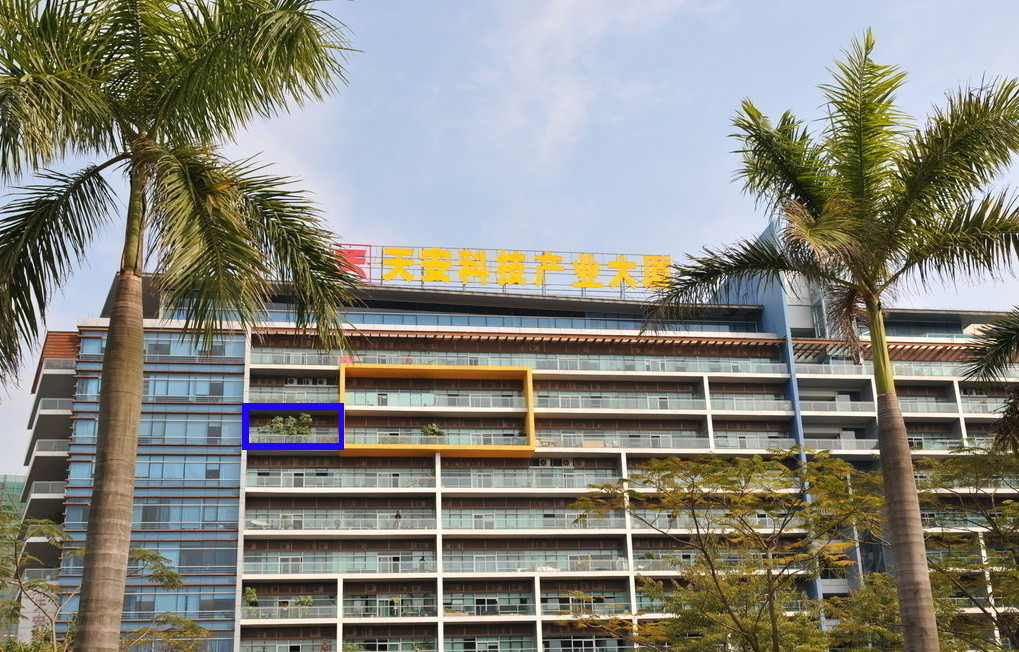
\includegraphics[width=5cm]{chap02/building}
        \centerline{(a) 建筑物}\medskip
    \end{minipage}
  \begin{minipage}[b]{0.48\textwidth}
    \centering
    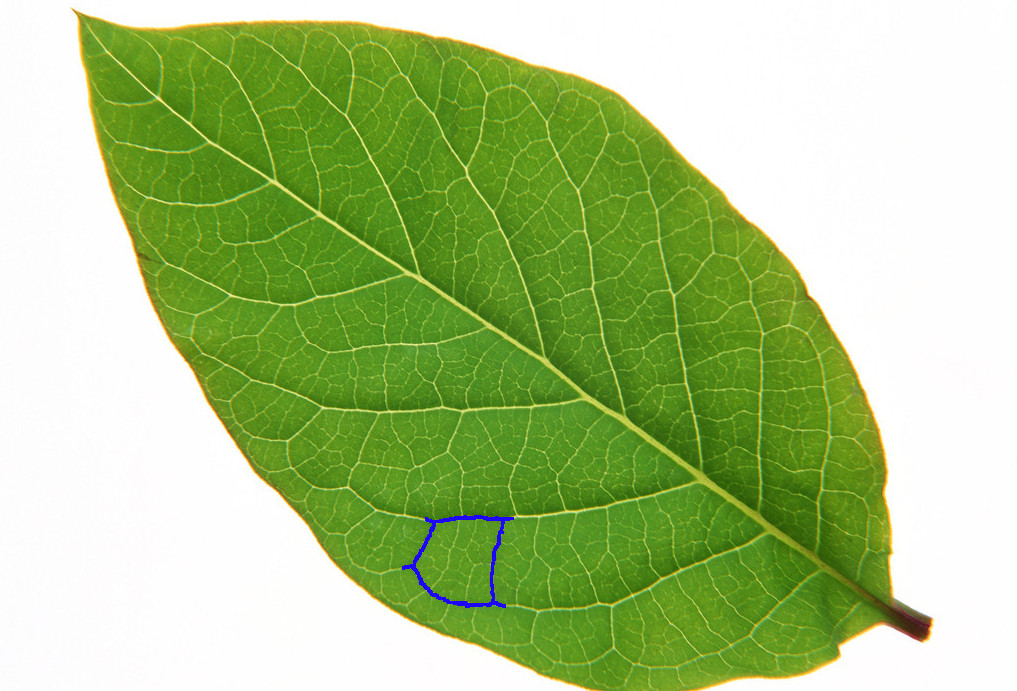
\includegraphics[width=5cm]{chap02/reaf}
      \centerline{(b) 树叶}\medskip
  \end{minipage}
  \begin{minipage}[b]{0.48\textwidth}
    \centering
    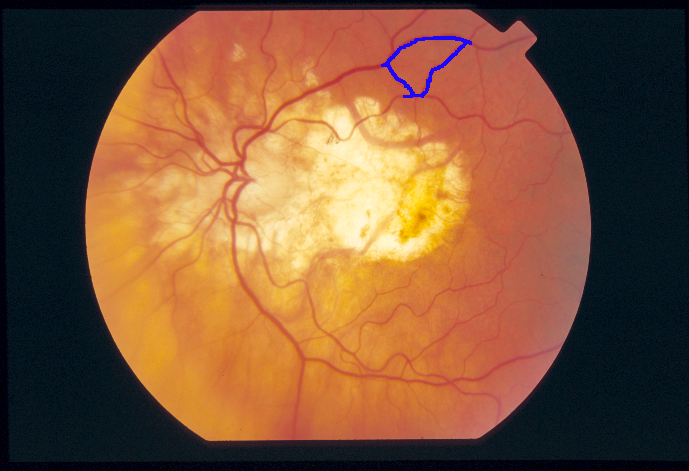
\includegraphics[width=5cm]{chap02/retinal}
      \centerline{(c) 视网膜}\medskip
  \end{minipage}
  \begin{minipage}[b]{0.48\textwidth}
    \centering
    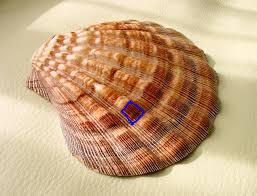
\includegraphics[width=5cm]{chap02/scallop}
      \centerline{(d) 扇贝}\medskip
  \end{minipage}
\caption{图像中的环结构}
\label{fig:Example}
\end{figure}




\section{预处理}
\label{}

原始图像一般都是灰度或彩色图像,若想从中提取环结构来用做识别或配准的特征,需要对其进行预处理,以使得环结构特征更加突出,以便能够准确快速的提取。对于原始图像的预处理主要分为四步,即基于偏微分方程的多尺度图像分割、连通区域标记图像去噪、膨胀腐蚀操作填充孔洞、骨架化,如图\ref{fig:Preprocessing}所示。经过这四步处理,原始图像转化为骨架化后的二值图像,以便进行环结构特征的提取。
\begin{figure}[H]
\centering
    \centering
    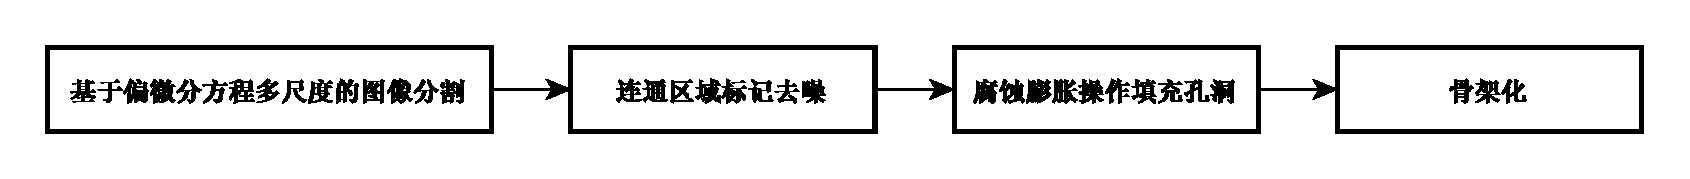
\includegraphics[width=13cm]{chap02/preprocessing}\medskip
\caption{预处理流程图}
\label{fig:Preprocessing}
\end{figure}
\subsection{基于偏微分方程的多尺度图像分割}

图像分割是计算机视觉领域的至关重要的技术,是介于图像分析与低层图像处理之间的图像处理过程,因而图像分割的结果好坏将很大程度上影响后续对图像的处理及应用。近些年来,对图像分割技术的研究层出不穷,分为基于区域的分割,基于边缘的分割,基于特定理论的分割,如基于模糊理论的分割、基于水平集的分割、基于活动轮廓的分割、基于图论的分割\cite{xuxiaoli}等等。

环结构特征存在于很多类图像中,不同类图像的环结构之间有很大的不同。例如,视网膜血管图像中血管较细、直径宽度变化范围大,血管与背景对比度低,扇贝贝壳纹理图像中边缘较模糊等,这就增加了图像分割的难度。为了减小图像分割对图像配准或识别的影响,并且使分割结果能够适用于多类不同图像,我们采用了基于偏微分方程多尺度的图像分割。

基于偏微分方程的多尺度图像分割\cite{wang2013retinal}不需要预处理与训练,可直接用于各类图像的分割。首先,利用多小波核对不同边缘的反映特性的不同,对图像中的边缘进行增强。通过多尺度多层分解方法对归一化的图像进行处理,以达到去除噪声和定位边缘的目的。尺度不同表示边缘的细化程度不同。最后,采用自适应阈值方法得到分割后的二值图像,图\ref{fig:flow-segmentation}为基本流程图。这样一幅图像就得到了不同尺度的多个分割结果,针对不同的应用问题就可以选择不同的尺度进行后续处理。

\begin{figure}[H]
\centering
    \centering
    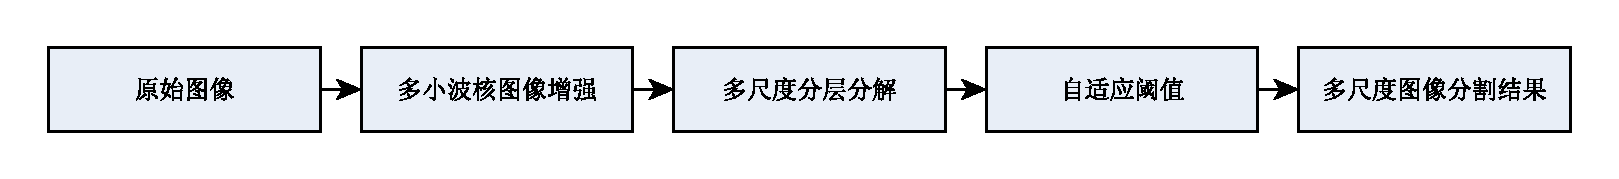
\includegraphics[width=13cm]{chap02/flow-chart-segmentation}\medskip
\caption{多尺度图像分割流程图}
\label{fig:flow-segmentation}
\end{figure}

二维多小波核$ker(x,y;a,b)$可以表示为:
\begin{eqnarray}
k_1(x,y;a,b)&=&\phi_1\{a^{-1}(x-b)\}\\
k_2(x,y;a,b)&=&\phi_2\{a^{-1}(x-b)\}\\
|y| &\geq& L/2
\end{eqnarray}
其中, $(x,y), \phi_i,a,b$及L分别表示像素坐标,一维多小波核尺度函数,尺度参数,平移参数,及二位多小波核在y方向的长度。

二维多小波核对二维图像进行匹配滤波实际上就是通过多小波核对图像进行卷积运算的结果,通过对多小波核进行任意角度旋转,然后与图像进行卷积,求最大值,可以得到:
\begin{equation}
M_{ker}(x,y;a,b) = max_\theta(r_\theta(ker(x,y;a,b)) \ast Img(x,y))
\end{equation} 

$r_\theta$表示将多小波核旋转$\theta$角度后得到的结果,$\ast$表示卷积运算。

图像中物体的轮廓或边缘的增强,通过计算多小波核$k_1(x,y;a,b)$与图像最大卷积得到:
\begin{equation}
M_{k_1}(x,y;a,b) = max_\theta(r_\theta(k_1(x,y;a,b)) \ast Img(x,y))
\end{equation} 

多小波核$k_2(x,y;a,b)$与图像局部平均最大卷积可用来增强图像背景:
\begin{eqnarray}
M_{k_2}(x,y;a,b) &=& max_\theta(D_m(r_\theta(k_2(x,y;a,b)) \ast Img(x,y)))\\
D_m(Img) &=& Img\ast W
\end{eqnarray} 
其中,$D_m$表示图像的局部平均,W表示一个$w \times w$的滤波器。通过多小波核匹配滤波器的处理,图像中的物体得到增强,并且可与非物体进行区分。

多尺度分层分解是迭代分割的过程,在这个迭代的过程中,越来越多的信息能够被检测到,通过尺度参数可以控制分割的精细程度。

分解模型的数值实现,实质上是最小化欧拉-拉格朗日方程$J(f,\lambda)$的过程:
\begin{equation}
u_\lambda - \frac{1}{2\lambda}div(\frac{\bigtriangledown_{u_\lambda}}{|\bigtriangledown_{u_\lambda}|})
\end{equation}
诺伊曼边界条件为:
\begin{equation}
\frac{\partial_{u_\lambda}}{\partial_n} = 0 \qquad \textrm{on} \qquad \partial \Omega
\end{equation}
其中,n是边界$\partial \Omega$的外法线。通过Gauss-Seidel迭代法\cite{tadmor,nezzar}可以来求解方程。

为了得到二值化的图像分割结果,采用自适应阈值的方法,该方法把边缘的过零点作为插值点得到图像阈值平面。图像的不同区域的二值化阈值不同。通过顺序松弛算法,可以得到u的阈值平面$\bar{u}$。则二值化公式为:

\begin{align}
Out(x,y) = \left\{ \begin{array}{ll}
1 & \bar{u}(x,y)\leq u(x,y)\\
0 & \textrm{其他}
\end{array} \right.
\end{align}
Out为最终得到的二值化图像。

图\ref{fig:Segmentaion-retinal}显示了视网膜图像的三个不同尺度的分割结果,a为原图,b、c、d分别为不同尺度的分割结果。从图中可以看出,从图b到图d,越来越多的血管被分割出来。b图中只分割出了原图中较为粗的血管,图d分割出了更为精细的血管。但从d图中可以看出分割的越精细,噪声也越大。图\ref{fig:Segmentaion-retinal1}是一组树叶图像的例子。可以很明显地看出从图b到图d,图像的细节信息越来越多地被分割出来。通过多尺度分割算法,可以得到图像不同层面的信息,这样,针对不同种类的图像的应用问题,就可以选择合适的分割尺度得到最佳的分割结果。

\begin{figure}
\centering
  \begin{minipage}[b]{0.48\textwidth} 
      \centering 
      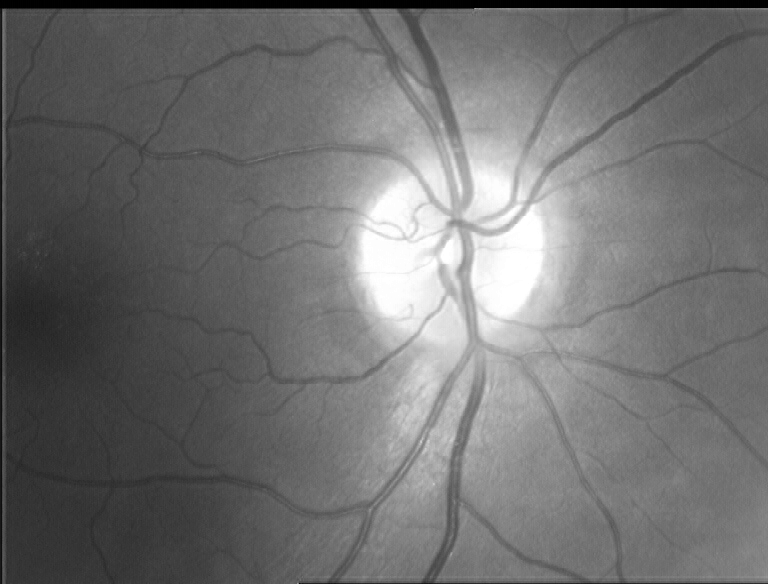
\includegraphics[width=6cm]{chap02/118}
        \centerline{(a)}\medskip
    \end{minipage}
  \begin{minipage}[b]{0.48\textwidth}
    \centering
    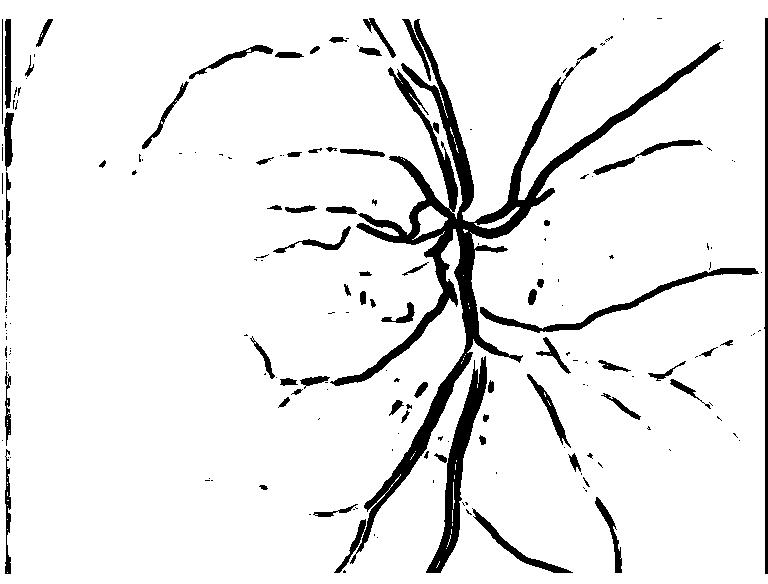
\includegraphics[width=6cm]{chap02/118-13}
      \centerline{(b)}\medskip
  \end{minipage}
  \begin{minipage}[b]{0.48\textwidth}
    \centering
    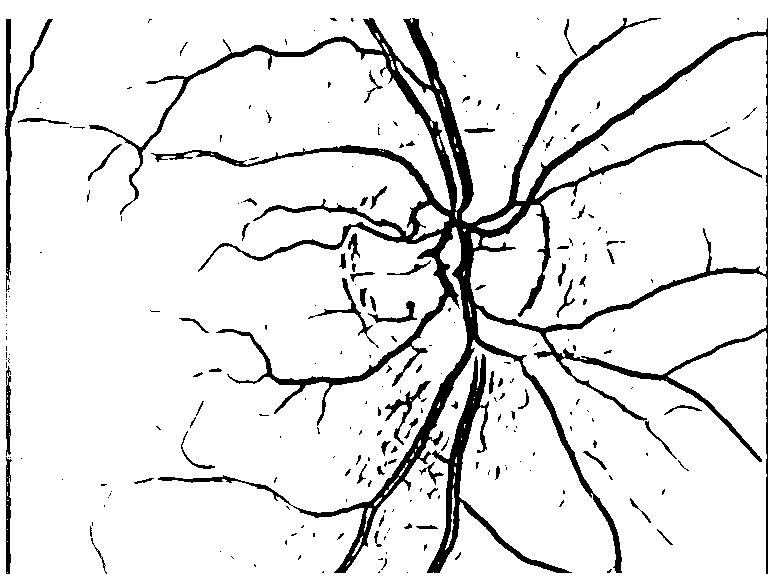
\includegraphics[width=6cm]{chap02/118-08}
      \centerline{(c)}\medskip
  \end{minipage}
  \begin{minipage}[b]{0.48\textwidth}
    \centering
    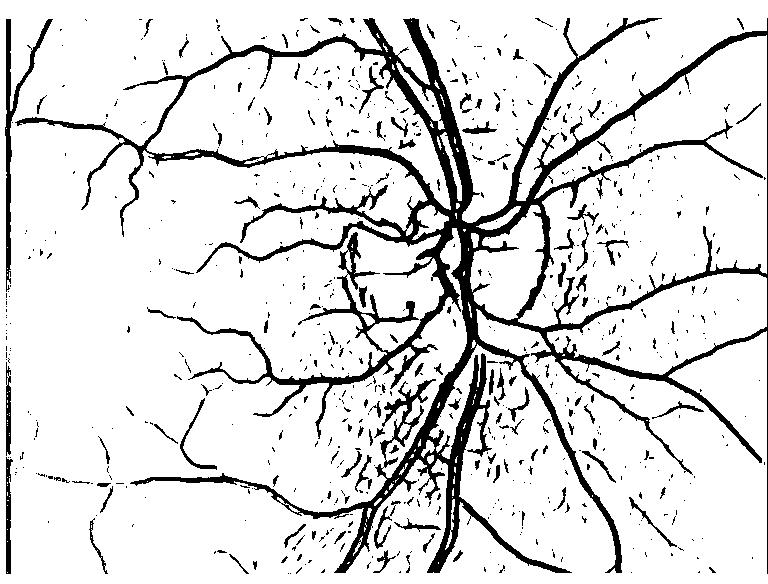
\includegraphics[width=6cm]{chap02/118-01}
      \centerline{(d)}\medskip
	\label{fig:max}
  \end{minipage}
\caption{不同尺度的视网膜图像分割结果。a为原图,b、c、d分别代表不同尺度的分割结果。}
\label{fig:Segmentaion-retinal}
\end{figure}

\begin{figure}
\centering
  \begin{minipage}[b]{0.48\textwidth} 
      \centering 
      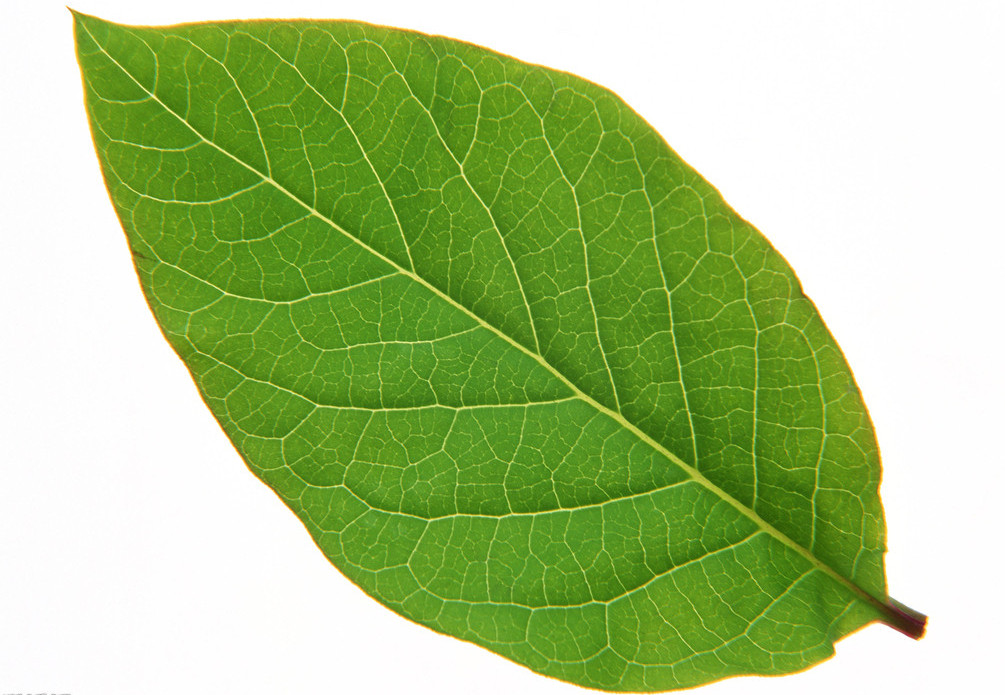
\includegraphics[width=6cm]{chap02/reaf-origin}
        \centerline{(a)}\medskip
    \end{minipage}
  \begin{minipage}[b]{0.48\textwidth}
    \centering
    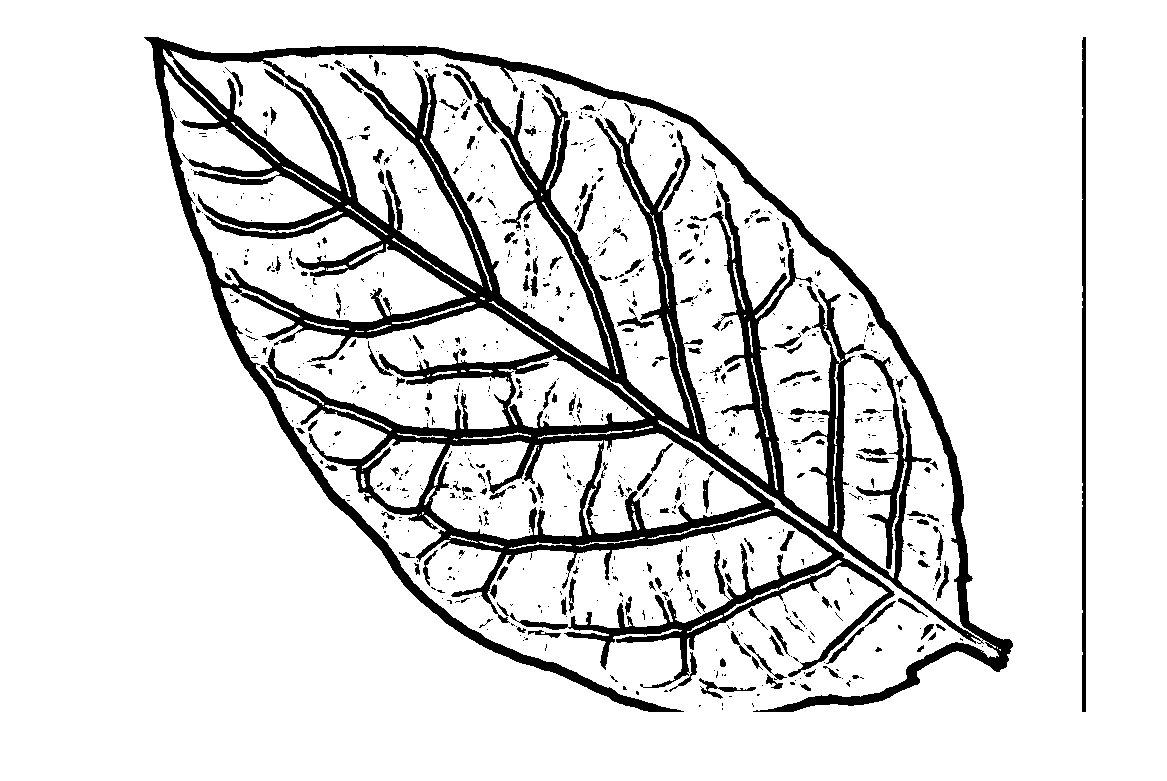
\includegraphics[width=6cm]{chap02/reaf1}
      \centerline{(b)}\medskip
  \end{minipage}
  \begin{minipage}[b]{0.48\textwidth}
    \centering
    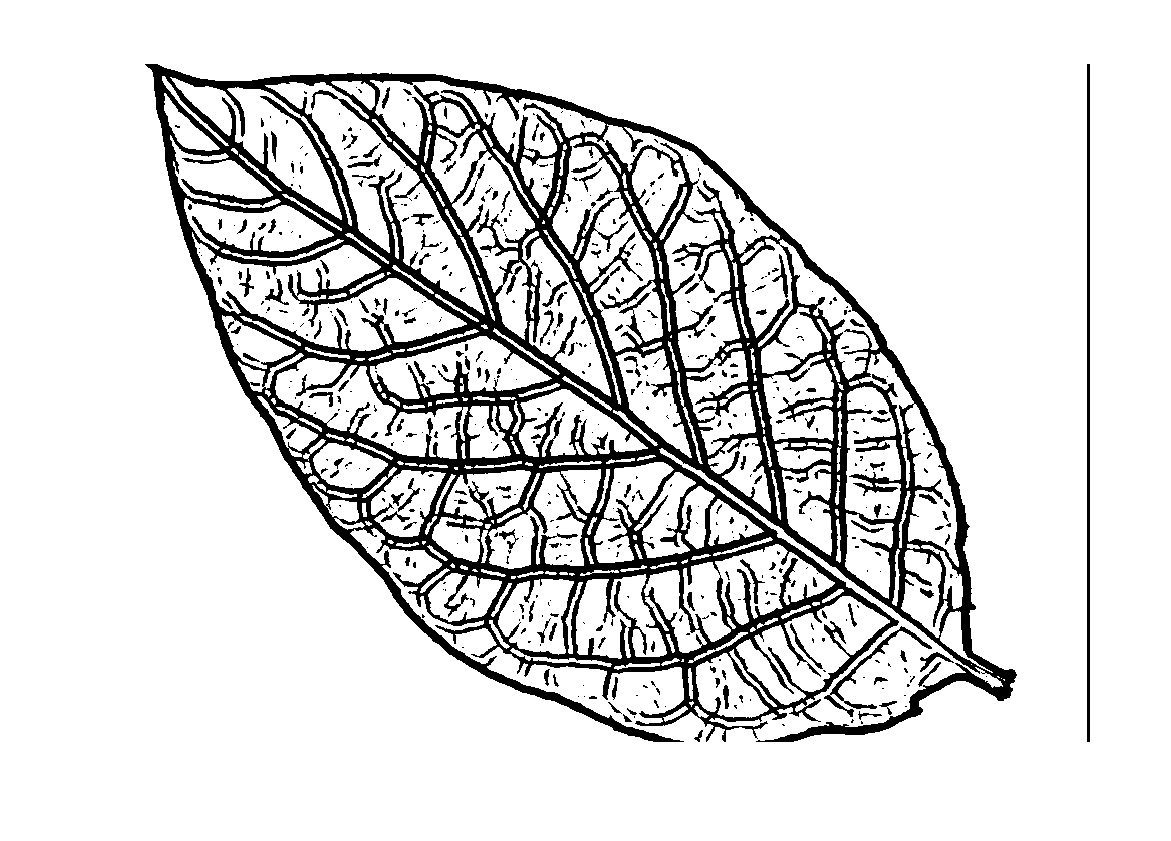
\includegraphics[width=6cm]{chap02/reaf3}
      \centerline{(c)}\medskip
  \end{minipage}
  \begin{minipage}[b]{0.48\textwidth}
    \centering
    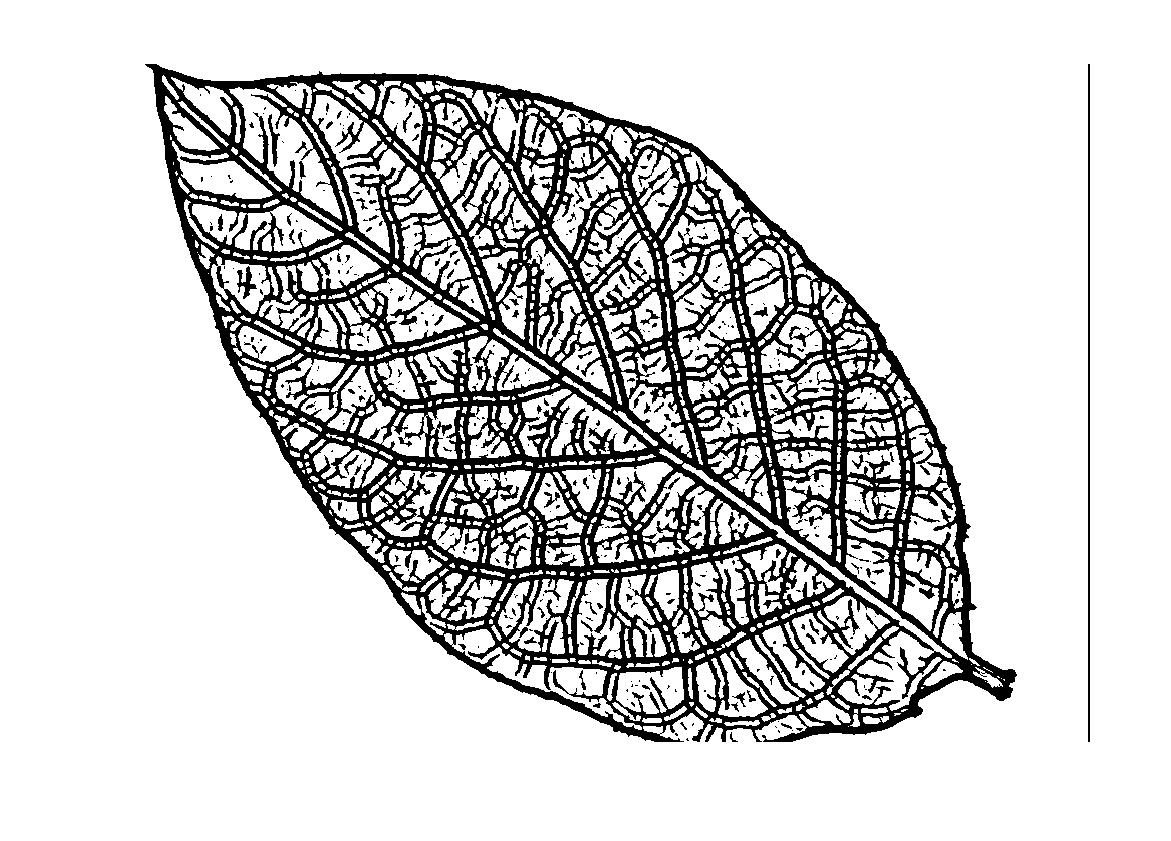
\includegraphics[width=6cm]{chap02/reaf2}
      \centerline{(d)}\medskip
	\label{fig:max}
  \end{minipage}
\caption{不同尺度的树叶图像分割结果。a为原图,b、c、d分别代表不同尺度的分割结果}
\label{fig:Segmentaion-retinal1}
\end{figure}

然而,若原图亮度不均或背景中存在较大噪声,分割尺度较大时虽然会把图像的细节分割出来,但噪声也会随之被分割出来,这样就增加环结构提取的困难度。为了消除噪声对环结构提取的影响,要对分割后的图像进行去噪处理。

\subsection{连通区域标记图像去噪}

连通区域标记\cite{xuzhengguang}是图像处理中常用的一个基本方法,在目标分割、边缘检测中有着十分广泛的应用。同时,连通区域也可应用于图像去噪。
采用连通区域算法对连通区域进行标记,即通过对二值图像进行逐行逐列扫描,根据图像中像素之间的邻域关系,对属于同一四连通或八连通区域的像素赋予相同的标号,然后统计同一标号的像素的个数。若像素数小于某个阈值,则认为是噪声。

邻域关系有两种,即四邻域与八邻域。设像素$P(x, y)$,则像素P的四邻域表示为$P_1(x,y-1), P_2(x, y+1), P_3(x-1,y), P_4(x+1,y)$,像素P的八邻域表示为$P_1(x,y-1), P_2(x, y+1), P_3(x-1,y), P_4(x+1,y), P_5(x-1,y-1), P_6(x+1, y+1), P_7(x-1,y+1), P_8(x+1, y-1)$,更加直观的表示如表\ref{tab:adjacent}。为了更好的去除噪声,我们采用八邻域去噪。
\begin{table}[H]
\centering
\caption{四邻域与八邻域}
\begin{tabular}{|c|c|c|}
\hline
 & $P_1$ & \\
\hline            
$P_3$ & $P$ & $P_4$\\
\hline           
& $P_2$ & \\
\hline
\end{tabular}
\begin{tabular}{|c|c|c|}
\hline
$P_5$ & $P_1$ & $P_7$\\
\hline            
$P_3$ & $P$ & $P_4$\\
\hline            
$P_8$& $P_2$ & $P_6$ \\
\hline
\end{tabular}

\label{tab:adjacent}
\end{table}


图\ref{fig:denoise-table}是一幅二值图像的连通区域标记图,从图中可以看出,共有2个连通区域,标号为1、2。其中连通区域1只有两个像素,连通区域2有11个像素,若设定10个像素为基准,小于10个像素的连通区域为噪声,则连通区域1将被认为是噪声,进行去除,而连通区域2将被保留。\ref{fig:Preprocessing}(b)是图\ref{fig:Preprocessing}(a)经过去噪后的结果,从图中可以看出很多的噪声都被滤除了。这一步骤不仅会减小环提取过程的复杂性,也避免了噪声形成的假环结构被提取出来的情况。


\begin{figure}[H] % use float package if you want it here
  \centering
  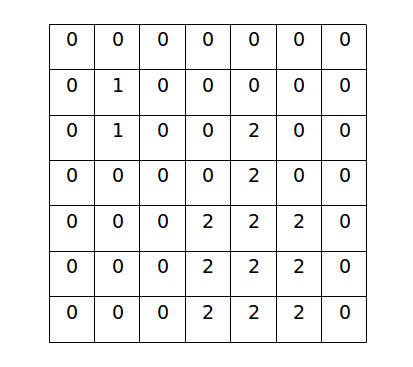
\includegraphics[width=0.4\textwidth]{chap02/denoise-table}
  \caption{连通区域标记去噪。区域1只有两个像素,若设置10个像素为阈值,则1被认为是噪声,需被去除。}
  \label{fig:denoise-table}
\end{figure}



\subsection{膨胀腐蚀操作填充孔洞}
在有些情况下,有时图像的亮度值不均匀,这就造成了分割出的线是断裂的或有孔洞的情况,为了骨架化后的图像能准确的体现原图像的特征,需对分割后的图像进行先膨胀后腐蚀操作。
膨胀腐蚀是图像形态学中比较常见的处理,一般是对二值图像进行处理。
用b对函数f进行的灰度膨胀\cite{gang}表示为:
\begin{align}
(f\oplus b)(s,t)=max\{f(s-x, t-y)+b(x,y)|(s-x),(t-y)\in D_f;(x,y)\in D_b\}
\end{align}
其中,$D_f$和$D_b$分别是f和b的定义域。
灰度腐蚀表示为$f \ominus b$,定义为:
\begin{align}
(f \ominus b)(s,t)=min\{f(s+x, t+y)-b(x,y)|(s+x),(t+y)\in D_f;(x,y)\in D_b\}
\end{align}

图\ref{fig:peng-fu}显示了先膨胀后腐蚀与先腐蚀后膨胀的区别。a、d为原图,三个黑色矩形块之间的两个空隙分别为5个与10个像素,若采用$5\times5$的矩形窗口对图像进行膨胀腐蚀与腐蚀膨胀操作,得到的最终结果如图c与e。从图中可以看到,先膨胀后腐蚀后,狭窄的缝隙被填充了,而在此例中先腐蚀后膨胀后得到的结果与原图相同。视网膜图像的示例如图\ref{fig:Preprocessing}(c)所示,血管中心位置的孔洞被成功填充。

\begin{figure}
\centering
  \begin{minipage}[b]{0.3\textwidth} 
      \centering 
      
\includegraphics[width=6cm]{chap02/peng-origin}
        \centerline{(a)原图}\medskip
    \end{minipage}
  \begin{minipage}[b]{0.3\textwidth}
    \centering
    
\includegraphics[width=6cm]{chap02/peng-fu}
      \centerline{(b)膨胀}\medskip
  \end{minipage}
  \begin{minipage}[b]{0.3\textwidth}
    \centering
    
\includegraphics[width=6cm]{chap02/peng-fu}
      \centerline{(c)膨胀后腐蚀}\medskip
  \end{minipage}
   \begin{minipage}[b]{0.3\textwidth} 
      \centering 
      
\includegraphics[width=6cm]{chap02/peng-origin}
        \centerline{(d)原图}\medskip
    \end{minipage}
  \begin{minipage}[b]{0.3\textwidth}
    \centering
    
\includegraphics[width=6cm]{chap02/fu-peng1}
      \centerline{(e)腐蚀}\medskip
  \end{minipage}
  \begin{minipage}[b]{0.3\textwidth}
    \centering
    
\includegraphics[width=6cm]{chap02/fu-peng2}
      \centerline{(f)腐蚀后膨胀}\medskip
  \end{minipage}
\caption{先膨胀后腐蚀与先腐蚀后膨胀}
\label{fig:peng-fu}
\end{figure}

\subsection{骨架化}
为了获得一个像素宽的骨架化结果,我们采用轮廓修剪骨架提取方法~\footnote{http://www.cs.smith.edu/$\sim$nhowe/research/code/}。这个方法是Nicholas R. Howe实现的,想法是Alex Telea提出的。若一个点位于一个圆圈的中心,并接触一个图像边缘的多个点,灰度骨架化图像的强度是基于围绕图像的周长连接最远的两点的最短距离。因此,骨架中的毛刺是由微小的边缘扰动引起的强度变化。如果圆圈接触断裂的边缘,骨架化将会是无限的过程。最终的骨架化结果是通过噪声突起轮廓的预期大小来确定的阈值来决定的。图\ref{fig:Preprocessing}(d)是骨架化结果,从图中可以看到,骨架后的图像能准确的描绘出血管的主轮廓。
\begin{figure}[H]
\centering
  \begin{minipage}[b]{0.48\textwidth}
    \centering
    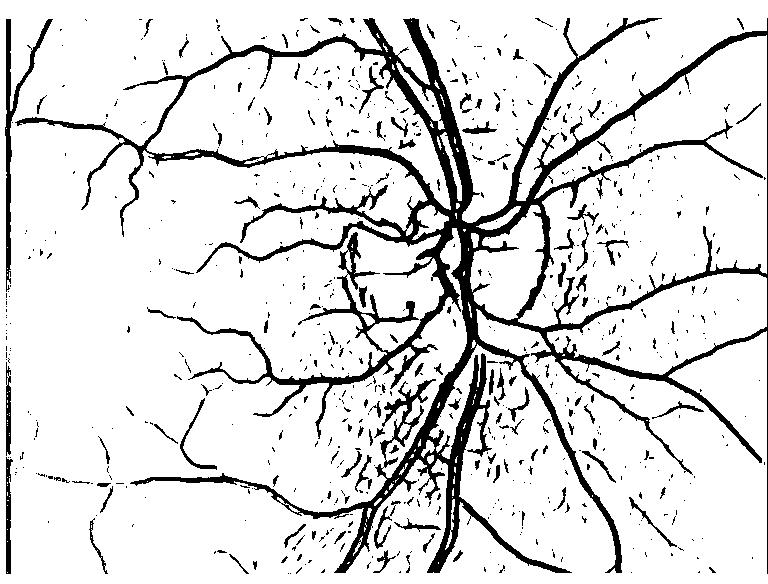
\includegraphics[width=6cm]{chap02/118-01}
      \centerline{(a) 分割图}\medskip
  \end{minipage}
  \begin{minipage}[b]{0.48\textwidth}
    \centering
    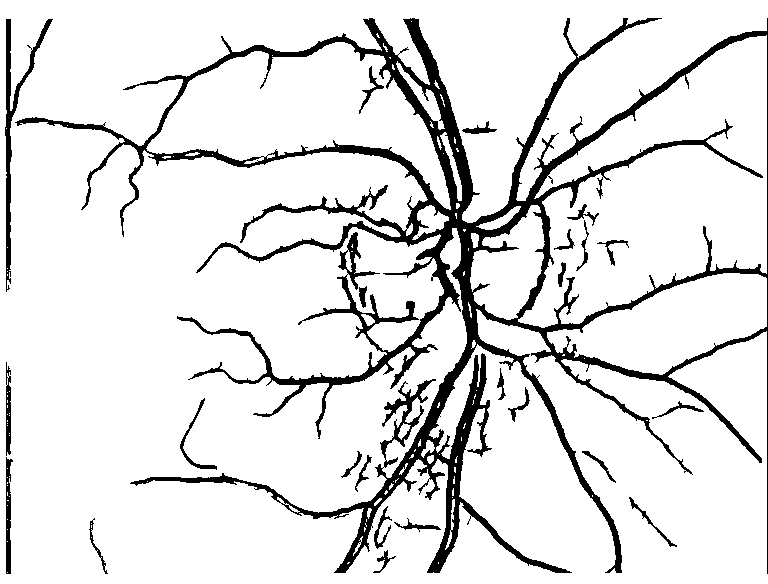
\includegraphics[width=6cm]{chap02/denoise}
      \centerline{(b) 去噪图}\medskip
  \end{minipage}
  \begin{minipage}[b]{0.48\textwidth}
    \centering
    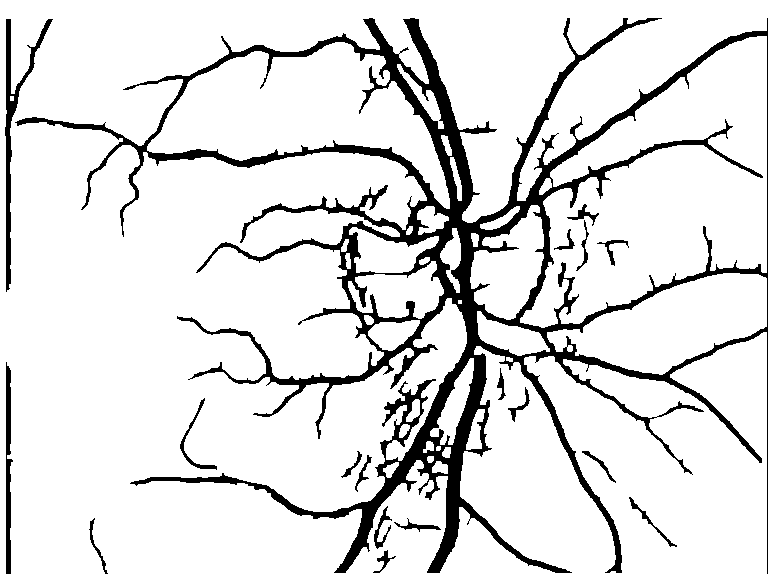
\includegraphics[width=6cm]{chap02/fill}
      \centerline{(c) 填充图}\medskip
  \end{minipage}
  \begin{minipage}[b]{0.48\textwidth}
    \centering
    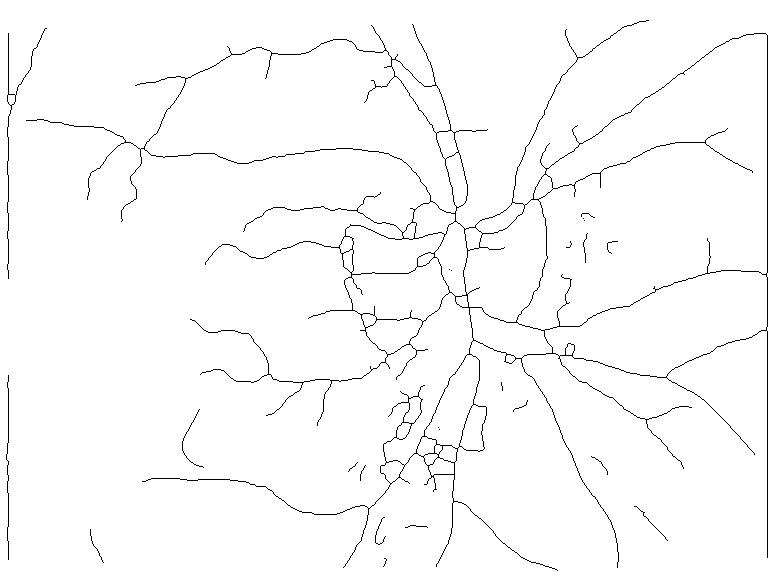
\includegraphics[width=6cm]{chap02/118-skel}
      \centerline{(d) 骨架图}\medskip
  \end{minipage}
\caption{预处理}
\label{fig:Preprocessing}
\end{figure}

经过这四个步骤,各类彩色图像就变为去噪后的骨架化二值图像,其中的环结构具有一个像素宽度,这样就为检测环结构做好了准备。

\section{环结构检测}
\label{}
\subsection{图论相关概念}
\label{}

图像中环的概念是由图论扩展而来的。在人类社会的实际生活中,有时在描述某些事物或对象之间有某种特定关系时采用图形的方式显得更加直观。对象用图形中的点表示,两对象之间具有的某种特定的关系用两点之间的无向或有向连线表示,由此数学抽象产成了图的概念。

\begin{definition}
一个图$G$定义为一个数学结构$(V, E, \phi)$\cite{xujunming},其中
\begin{enumerate}
\item $V$是一个集合,其中的元素成为顶点;
\item $E$是定义在$V$上的可以重复的二元关系集,其中的元素成为边;
\item $\phi$ 是$E$到$V$的一个映射。 
\end{enumerate}
若$\phi(E)$中的元素全是有序对,则$(V, E, \phi)$成为有向图,否则,成为无向图。我们所研究的图像中的线是无方向的,所以我们可以把图像认为是无向图。
\end{definition}

在图像中,顶点可以定义为线的交叉、分叉点或孤立点,边为连接两个顶点的连线,如图\ref{fig:graph}所示,$V = \{v_1, v_2, v_3, v_4, v_5\}$,$E = \{e_1, e_2, e_3, e_4\}$,边$e_1$把顶点$v_1, v_2$连接起来。

\begin{figure}[H] % use float package if you want it here
  \centering
  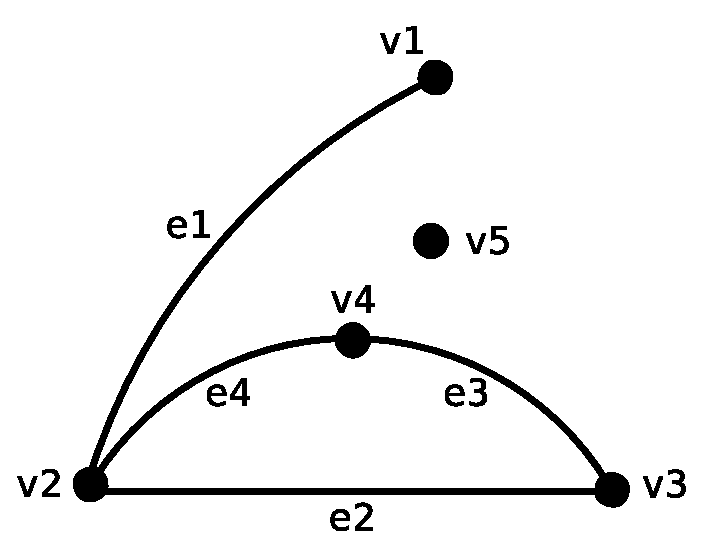
\includegraphics[width=0.3\textwidth]{chap02/graph}
  \caption{图}
  \label{fig:graph}
\end{figure}

\begin{definition}
设$G$是无向图,$x\in V(G)$的顶点度定义为$G$中与$x$关联边的数目,记为$d_{G}(x)$\cite{wangshuhe}。
\end{definition}

图\ref{fig:graph}中,只有一条边$e_1$与顶点$v_1$相连,即$d_{v_1}=1$,类似的,$d_{v_2}=3, d_{v_5}=0$。


\begin{definition}
设无向图$G = (V, E), v_i, v_j \in V$,若存在一条边$e$以$v_i, v_j$为端点,即$e = (v_i, v_j)$,则称$v_i, v_j$是彼此相邻的,简称相邻的。 
\end{definition}
例如,图\ref{fig:graph}中,$v_1$与$v_2$是相邻的,$v_2$与$v_5$是不相邻的。

设$(V, E, \phi)$是无向图$G$,其中$V = \{v_1, v_2, \ldots, v_p\}$,$E = \{e_1, e_2, \ldots, e_\varepsilon\}$。则无向图G的邻接矩阵能够反映出V中元素与E中元素之间的关联关系。
\begin{definition}
设图G的顶点集$V = \{v_1, v_2, \ldots, v_p\}$,令
\begin{align}
a_{ij} = \left\{ \begin{array}{ll}
1 & \textrm{$v_i$与$v_j$相邻}\\
0 & \textrm{$v_i$与$v_j$不相邻或$i = j$}
\end{array} \right.
\end{align}
则称由元素$a_{ij} (i, j == 1, 2, \ldots, p)$构成的p阶矩阵为图G的邻接矩阵\cite{wangzhaorui},记作A。
\end{definition}
图\ref{fig:graph}的邻接矩阵是
\begin{align}
A = \left( \begin{array}{lllll}
0 & 1 & 0 & 0 & 0 \\
1 & 0 & 1 & 1 & 0 \\
0 & 1 & 0 & 1 & 0 \\
0 & 1 & 1 & 0 & 0 \\
0 & 0 & 0 & 0 & 0 
\end{array} \right)
\end{align}

无向图中的环是指一系列边的集合,起始点与终止点是重合的。一些环的集合成为一个环基。在无向无权图中,环的权重为组成这个环的边的数量。最小环基就表示能使组成这个环基的权重的总和最小的环的集合。图\ref{fig:graph}中,共存在九个环,即:$c_1 = < v_1, v_2, v_3>, c_2 = <v_4, v_5, v_6>, c_3 = <v_5, v_6, v_7, v_8, v_{10}>, c_4 = <v_8, v_9, v_{10}>, c_5 = < c_{14}, c_{15}, c_{16}>, c_6 = <v_{10}, v_{11}, v_{12}, v_{13}>, c_7 = <c_4, c_5, v_{10}, v_9, v_8, v_7, v_6>, c_8 = < v_6, v_5, v_{10}, v_9, v_8, v_7>, v_9 = < v_4, v_5, v_{10}, v_9, v_8, v_7, v_6>$,其中,$c_1, c_2, c_3, c_4, c_5$是最小环,他们组成的集合为最小环基,即$M = \{c_1, c_2, c_3, c_4, c_5\}$。
\begin{figure}[H]
\centering
    \centering
    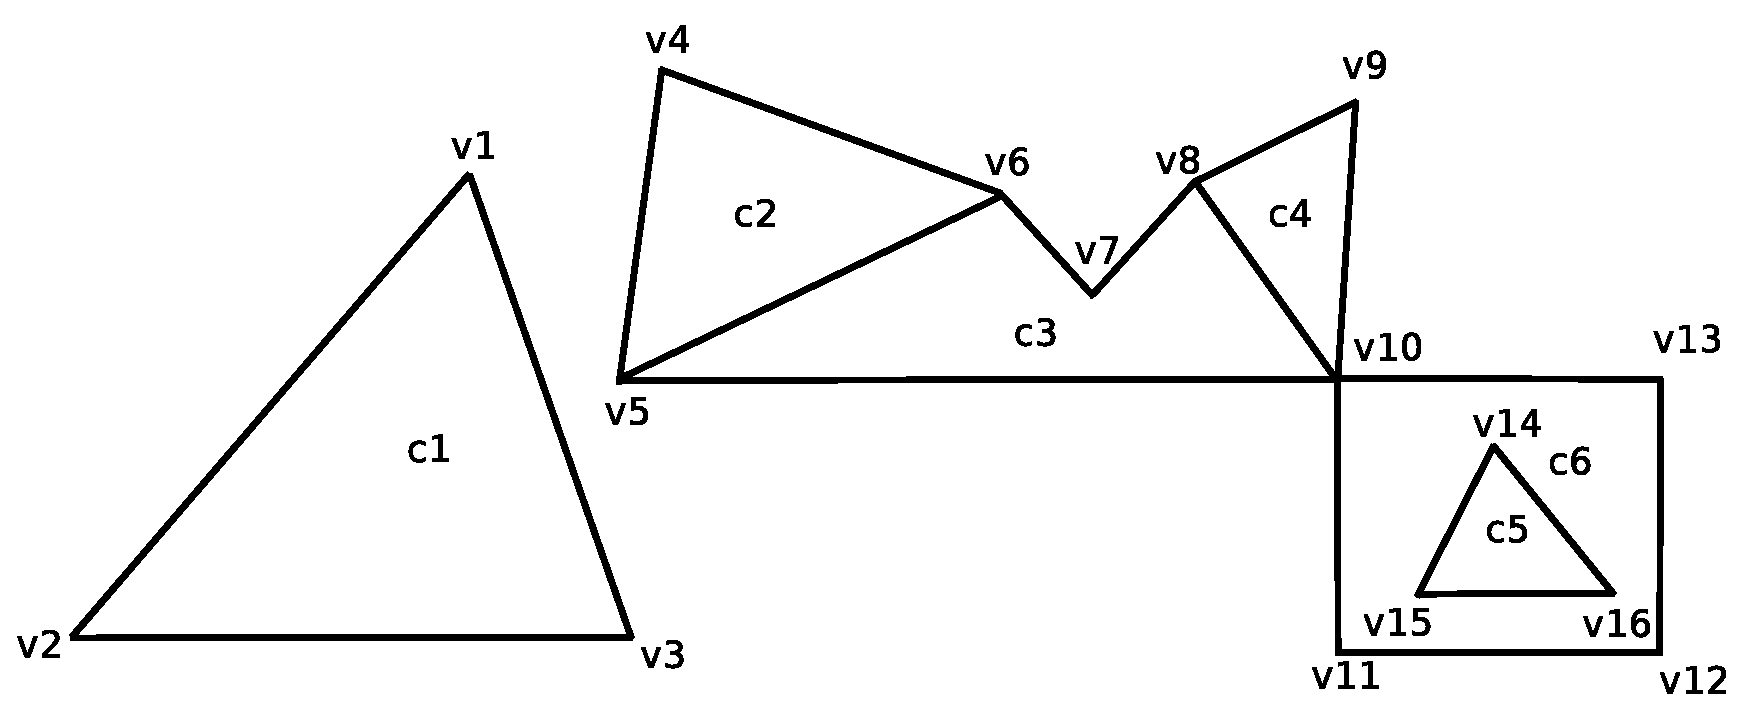
\includegraphics[width=10cm]{chap02/graph-cycle}\medskip
\caption{图中的环}
\label{fig:graph-cycle}
\end{figure}


检测图中的所有的环的问题,实际上就是检测图中的最小环基的问题。要在图像中检测最小环基,首先应先检测分叉点及其之间的连接关系,根据其连接关系,构造搜索路径,以此来实现检测环的过程。

\subsection{分叉点与连接关系检测}
\label{}

二值图像中,若背景为黑,即其像素值是0,线为白,即像素值是1。要判断一个像素点是否为分叉点,首先应定位线的位置,即判断像素值是否为1,然后判断这个像素点的八邻域像素为1的像素个数,若八邻域没有像素为1的像素,则认为是度为1的顶点,即孤立点,若八邻域有1个像素值为1的像素,则认为这两个点形成一条短线段,这些点都不认为是分叉点。这样研究对象为八邻域内有大于等于3个像素值为1的点。通过观察与实验发现若八邻域有3个像素值为1的像素,则中心点其八邻域像素值为1的点形成三分叉,中心点可被认为是三分叉点,如图\ref{fig:FeaturePoints}所示,图(a)中的红色点八邻域内有3个值为1的点,则红色点为三分叉点。三分叉点的常见情况如图\ref{fig:FeaturePoints-image}(a)所示。

而若某一点的八邻域有三个以上像素值为1的像素,则不能单纯的认为是几分叉点,如图\ref{fig:FeaturePoints}(b)所示是四分叉点的例子,红色点及蓝色点八邻域都有3个以上的值为1的点,但蓝色点不能认为是分叉点。

这种情况下,我们要进行连通区域标记。首先重新定位可能是分叉点的点,即其八邻域有3个以上像素值为1的点。然后要进行连通区域标记,图\ref{fig:FeaturePoints}(b)中的红色及蓝色点标记为一个区域,根据标记点的坐标,计算连通区域的中心位置,最后把中心位置点作为同一个连通区域的分叉点,而连通区域内的其他点为普通点,即红色点作为连通区域的中心,看作是真正的四分叉点。在图像中\ref{fig:FeaturePoints}(b)显示为\ref{fig:FeaturePoints-image}(b),通过计算,蓝色点为中心位置点,即四分叉点。

\begin{figure}
\centering
  \begin{minipage}[b]{0.48\textwidth} 
      \centering 
      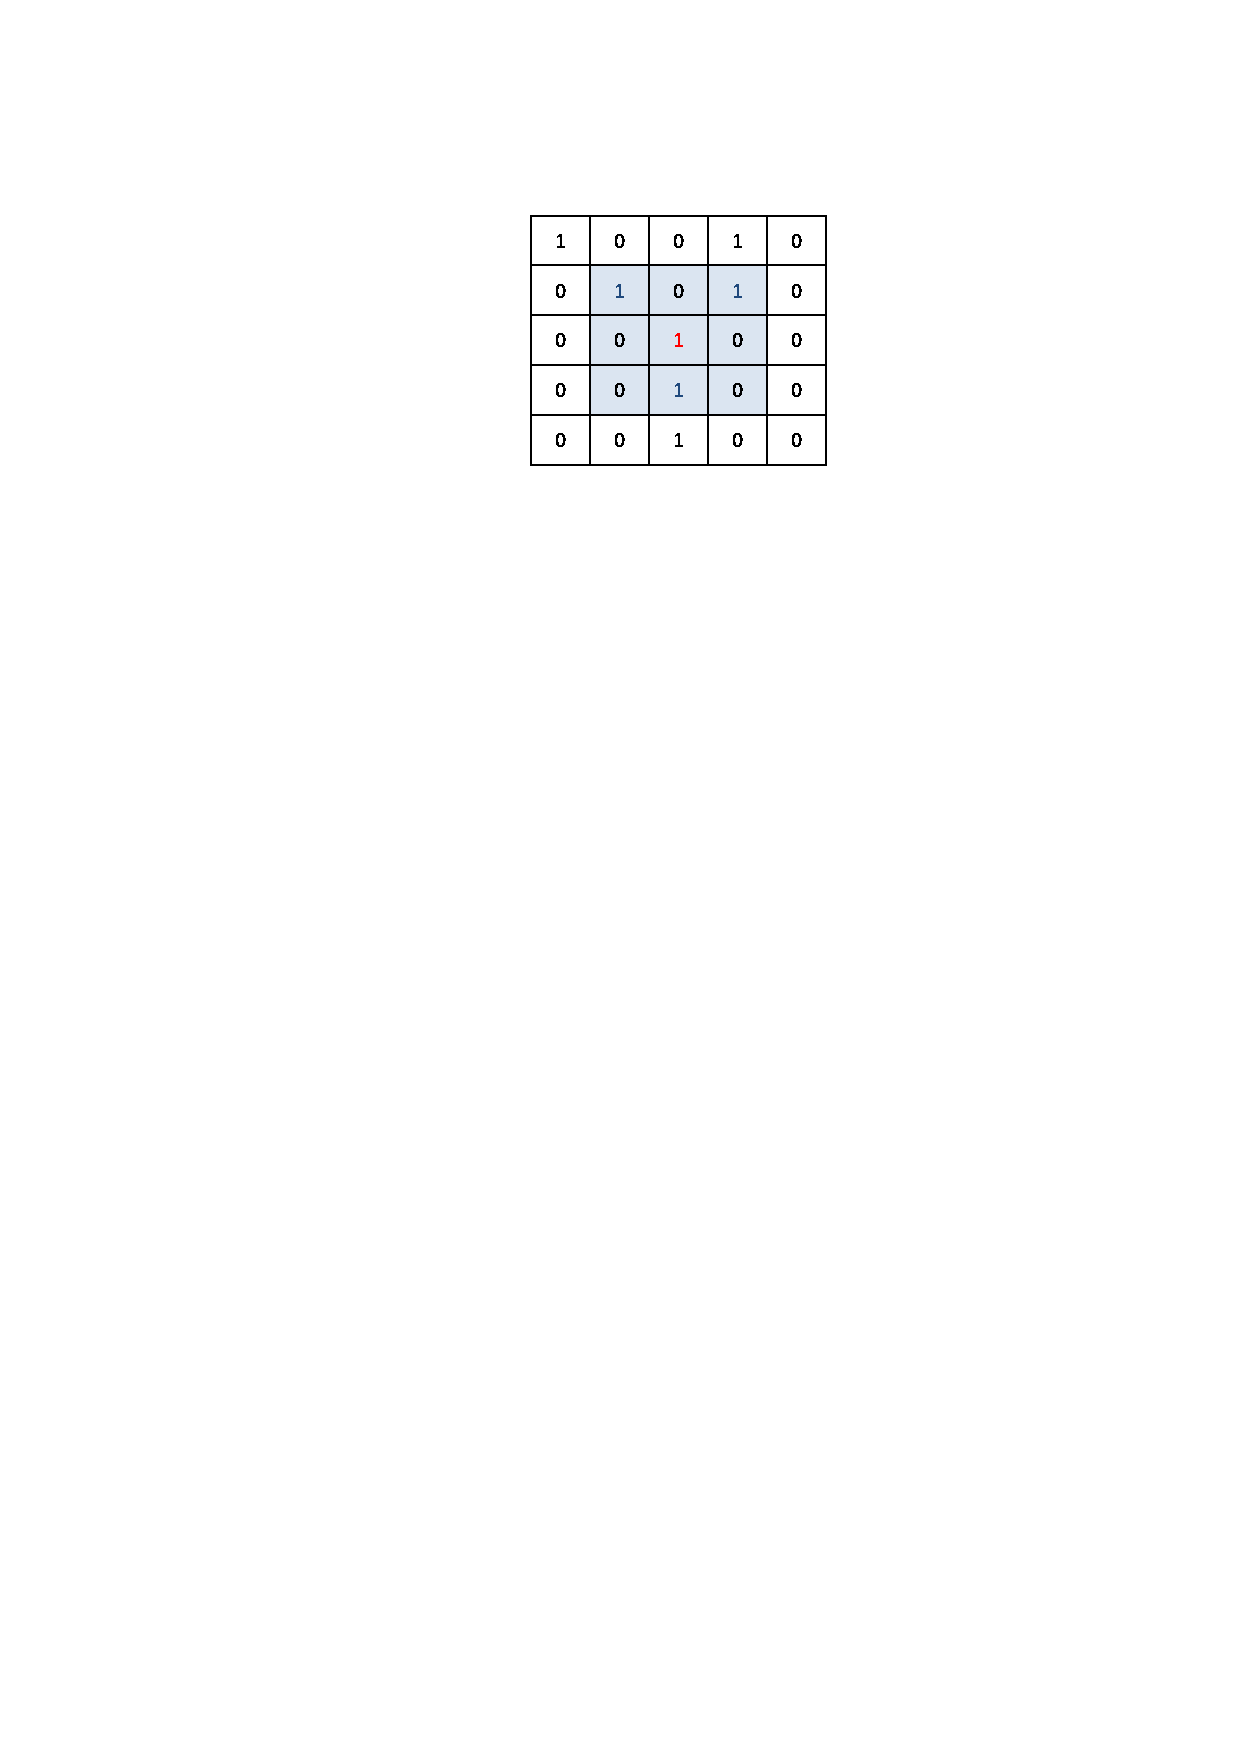
\includegraphics[width=4cm]{chap02/3FeaturePoint}
        \centerline{(a)}\medskip
	 \label{fig:3FeaturePoint}
    \end{minipage}
  \begin{minipage}[b]{0.48\textwidth}
    \centering
    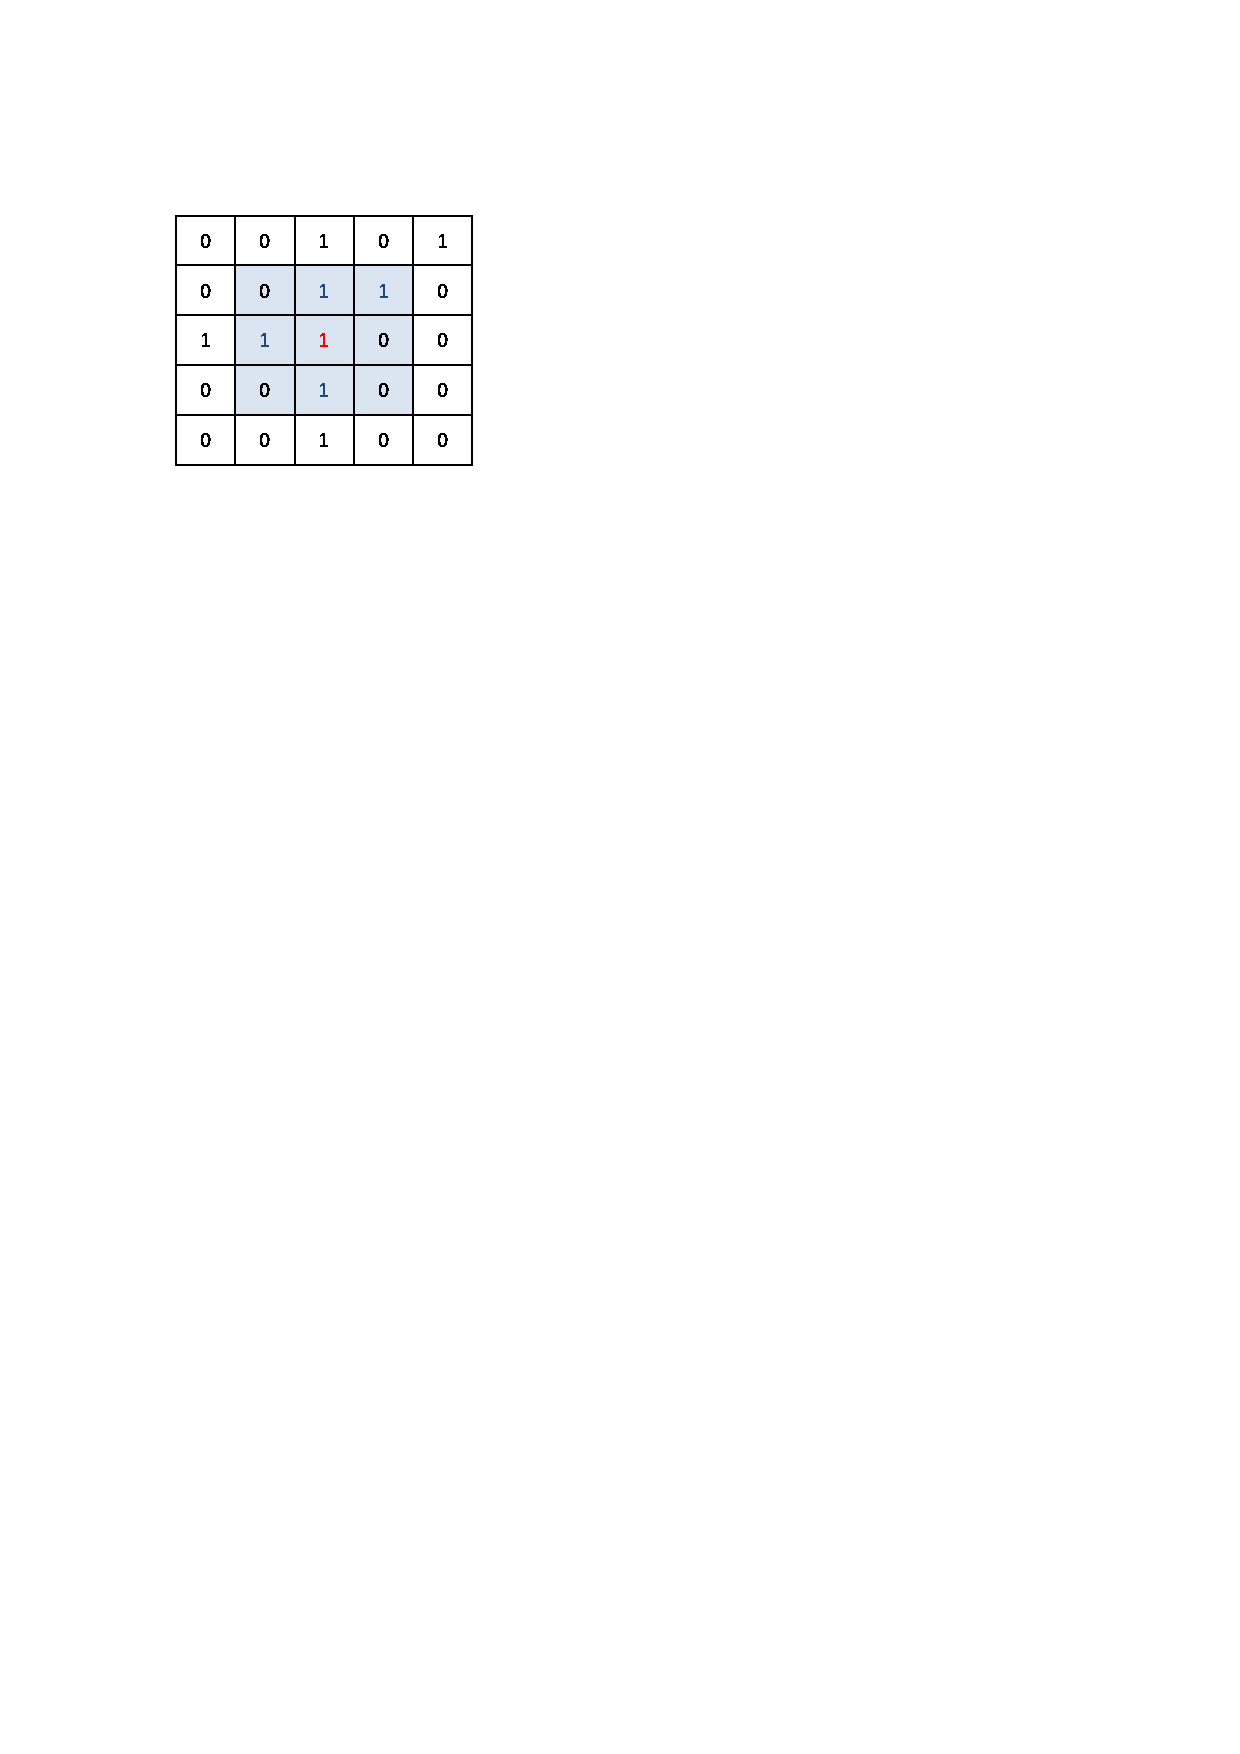
\includegraphics[width=4cm]{chap02/4FeaturePoint}
      \centerline{(b)}\medskip
	\label{fig:4FeaturePoint}
  \end{minipage}
\caption{三分叉点与四分叉点}
\label{fig:FeaturePoints}
\end{figure}

\begin{figure}
\centering
  \begin{minipage}[b]{1\textwidth} 
      \centering 
      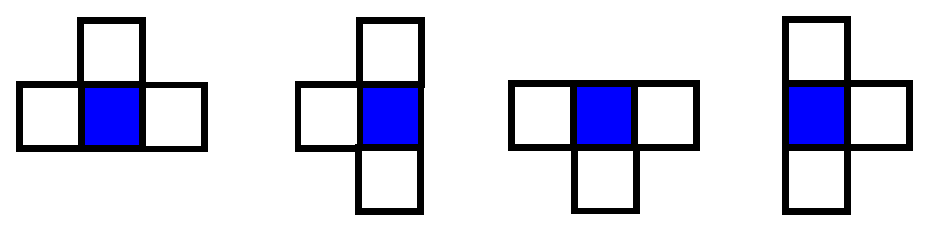
\includegraphics[width=8cm]{chap02/three-bifu}
        \centerline{(a)}\medskip
    \end{minipage}
  \begin{minipage}[b]{1\textwidth}
    \centering
    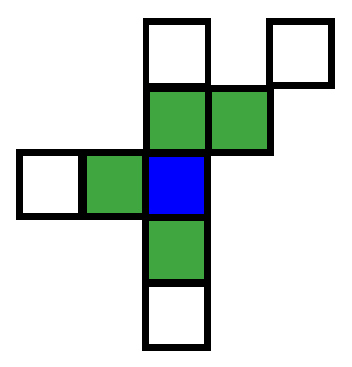
\includegraphics[width=3cm]{chap02/four-bifu}
      \centerline{(b)}\medskip
  \end{minipage}
\caption{三分叉点与四分叉点}
\label{fig:FeaturePoints-image}
\end{figure}

当所有的分叉点都检测到后,每个分叉点被看做一个种子,沿其八邻域像素值为1的方向不断向外扩展,直到找到与这个分叉点相邻的分叉点。遍历所有分叉点后,所有的分叉点及其连接关系就被检测到。为了方便后续操作,我们将采用顶点---边矩阵来表示分叉点及其连接关系,于是得到图\ref{fig:graph}的点---边关系表\ref{tab:AdjacentStructure},第一列为所有的分叉点,其余几列为与分叉点相连的分叉点。
\renewcommand\arraystretch{0.8}
\begin{table}[H]
\caption{点---边关系}
\centering
\begin{tabular}{p{2cm}<{\centering}p{1cm}<{\centering}p{1cm}<{\centering}p{1cm}<{\centering}}
  \hline
  分叉点 & \multicolumn{3}{c}{相邻分叉点}\\
  \hline
  \rowcolor{gray!50}
  $v_{1}$ & $v_{2}$  & $0$      & $0$  \\
  $v_{2}$ & $v_{1}$  & $v_{3}$  & $v_{4}$ \\
  \rowcolor{gray!50}
  $v_{3}$ & $v_{2}$  & $v_{4}$  & $0$\\
  $v_{4}$ & $v_{2}$  & $v_{3}$  & $0$ \\
  \rowcolor{gray!50}
  $v_{5}$ & $0$      & $0$      & $0$\\
  \hline
\end{tabular}
\label{tab:AdjacentStructure}
\end{table}

众所周知,能够组成环结构的分叉点数目至少为3,这就要求每个分叉点的度大于等于3,即$d_{v_i} \geq 3$,并且每个分叉点应至少在点---边关系矩阵中出现3次。通过这个规则,可以滤除一些不能组成环结构的点。但这个过程不能一次滤除所有的不能组成环结构的无效点,而是需要进行循环滤除,每进行一次,最外围的无效点将会滤除,直到所有的无效点被滤除后,循环得以结束。以一个视网膜图像为例,如图\ref{fig:Bifurcation},分别表示初始检测到的分叉点与所有无效分叉点被滤除后的图像,从图中可以看出,分支末端的点都被滤除,只剩下可能组成环的分叉点。通过滤除不能组成环的无效的分叉点,就可以大大的减少搜索环的路径,从而减小环检索算法的复杂度。

\begin{figure}
\centering
  \begin{minipage}[b]{0.48\textwidth} 
      \centering 
      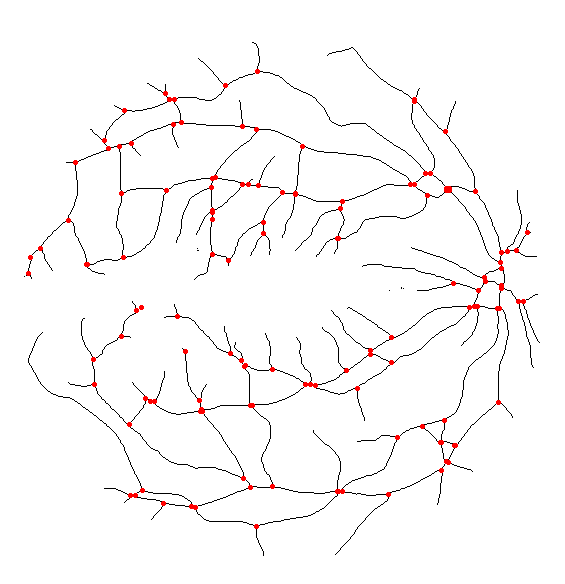
\includegraphics[width=4cm]{chap02/all-bifu}
        \centerline{(a)所有分叉点}\medskip
	 \label{fig:3FeaturePoint}
    \end{minipage}
  \begin{minipage}[b]{0.48\textwidth}
    \centering
    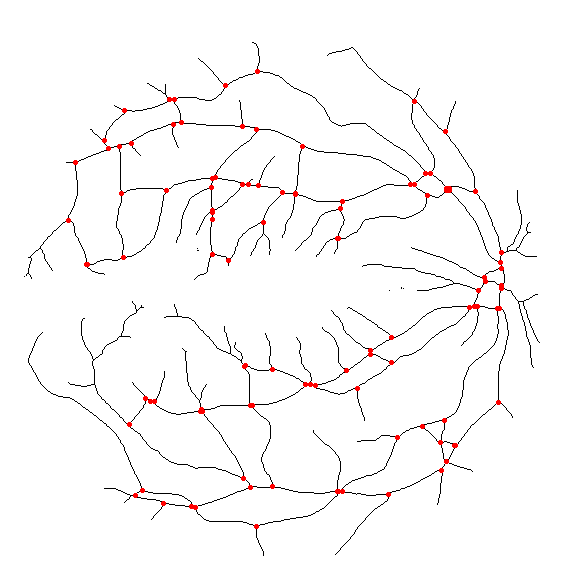
\includegraphics[width=4cm]{chap02/select-bifu}
      \centerline{(b) 可能组成环的分叉点}\medskip
	\label{fig:4FeaturePoint}
  \end{minipage}
\caption{所有分叉点与滤除无效分叉点后的对比图}
\label{fig:Bifurcation}
\end{figure}

\subsection{基于广度优先策略的环结构检测}
\label{}


在图中检测最小环基的问题实际上是图论中的一个被广泛研究的问题。Joe Kirk 提出了迭代环计数算法,算法的基本思想是通过动态路径搜索环,动态路径实际上是把图变换成一棵树,路径表示树上的一个结点到另一个结点的连线,当一个节点在一条路径上出现两次,则表示这条路径上的点形成一个环。

树的定义如下:
树是包括n个结点的有限集合$T(n \geq 1)$\cite{zhangming},使得
\begin{enumerate}
\item 有且只有一个特定的成为根的结点。
\item 除根以外的其他结点被分成m个$(m \geq 0)$个不相交的有限集合$T_1, T_2, \ldots, T_m$,而每一个集合又都是树。其中,树$T_1, T_2, \ldots, T_m$称作这个根的子树。
\end{enumerate}

这个定义是递归的,即在树的定义中又用到了树的概念。在一棵树中,若存在节点k指点个结点$k'$的连线,则称k是$k'$的父结点,而$k'$是k的子结点,有向连线$<k, k'>$称作边。同一个父结点的子结点之间称为兄弟。树中没有父结点的结点称为根,没有子结点的结点称为树叶。若树中存在结点序列$k_0,k_1,\ldots,k_s$,使得$<k_0,k_1>,<k_1,k_2>,\ldots,<k_{s-1},k_s>$都是树中的边,则称从结点$k_0$到结点$k_s$存在一条路径。若有一条由k到达$k_s$的路径,则称k是$k_s$的祖先,$k_s$是k的子孙。图\ref{fig:tree}表示一棵树,A表示根结点,B、C是A的子结点,A是BC的父结点,BC为兄弟结点。ABDI是一条路径,其中A是I的祖先,I为A的子孙。

\begin{figure}
\centering
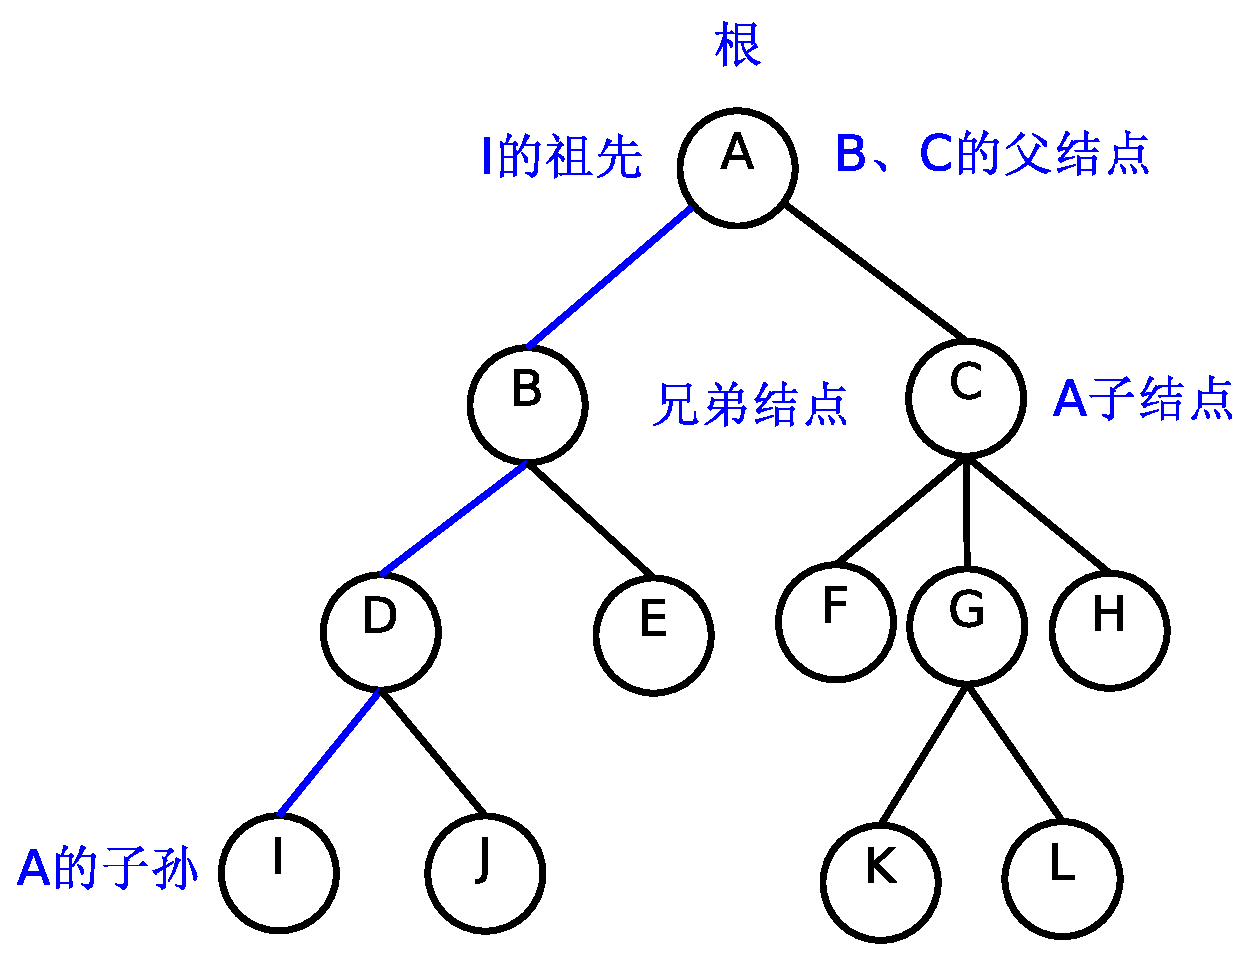
\includegraphics[width=0.5\textwidth]{chap02/tree-1}
\caption{树形表示法}
\label{fig:tree}
\end{figure}

在树中顺序搜索结点叫做树的遍历。通常有两种遍历方法:深度优先遍历与广度优先遍历。
\begin{itemize}

\item 深度优先遍历算法。深度优先算法的思想是尽可能沿分支结点向深度方向进行遍历。对于二叉树来说,深度优先即先沿着分支结点向左下降,当遇到左子树为空的时候,返回到上面最近的且其右子树尚未访问到的分支结点,转向该分支节点的右子结点,然后再尽可能地沿着左链前进。重复执行上述过程,直到遍历完所有的结点为止。

进行深度优先遍历时,结点既可以在向下遍历之前访问,也可以在从子树返回之后访问,根据结点的访问时间,可以定义不同的深度优先遍历算法,即前序法、中序法、后序法。前序法即先访问根结点,然后访问左子树,最后访问右子树。中序法先访问左子树,然后访问根结点,最后访问右子树。而后序法首先访问左子树,然后访问右子树,最后访问根结点。如图\ref{fig:dfs}所示为一个图,按前序法进行深度优先遍历时,访问结点的顺序应该是ABDECFG。

\item 广度优先遍历算法。广度优先又叫宽度优先或横向优先,是从上而下,从左到右地按层次进行遍历。其过程是:首先访问树的第一层,即根结点所在的层,然后从左到右依次访问第二层的结点,依次类推,当第i层的所有结点访问结束后,再从左到右依次访问第i+1层的各个结点。图\ref{fig:dfs}进行广度优先搜索的结果为ABCDEFG。

\end{itemize}

\begin{figure}[H]
\centering
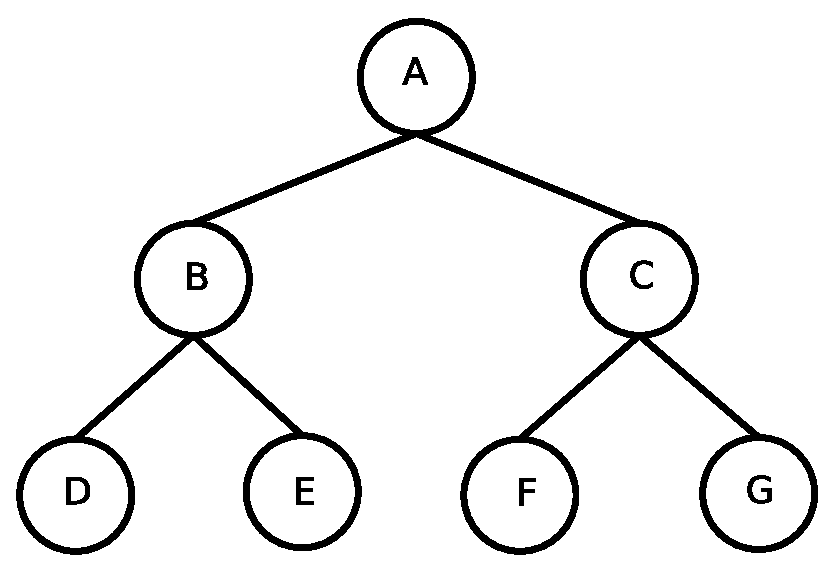
\includegraphics[width=0.4\textwidth]{chap02/dfs}
\caption{深度优先与广度优先}
\label{fig:dfs}
\end{figure}

迭代环计数算法也依赖于点---边关系矩阵,该算法利用了深度优先算法的思想,主要步骤为:
\begin{enumerate}
\item 初始化一个结点作为树的根。
\item 找到与这个结点相邻的结点,并把其中一个结点作为根的子结点,放入树的第二层。
\item 继续找与第二层中的点相邻的一个结点,作为树的第三层。在搜索根的子结点的相邻点的过程中,要排除其上一层中的点,即根结点不作为树的第三层中的点。
\item 若路径中包含两个相同的结点,则说明这个路径中的结点形成一个环,并继续按照点边关系寻找下一个结点。
\item 若没有环形成,则继续寻找下一个结点,并更新路径。
\item 若这条路径已经到最后一个结点,则回到树的上一层并更新路径。
\item 重复2到6步直到第8步完成。
\item 如果当前结点不是第一个结点,并且所有的结点都已搜索到则算法结束。
\end{enumerate}

如图\ref{fig:graph-tree},a表示一个图,b是根据迭代环计数算法转换成的树。首先初始化一个点1作为树的根,根据点边关系矩阵,搜索到1的子结点2,放入树的第二层,根据2的点边关系矩阵,搜索到3结点,放入树的第三层,继续搜索3的点边关系矩阵,得到结点1,此时结点1、2、3、1形成一个环结构,然后回溯到1的上一层,即第三层继续寻找除1以外与3相连的其他点,即4点,然后继续搜索,直到遍历所有的点边关系矩阵。由此,遍历结束后,得到三个环结构,即123、1243、243。重复搜索的环将在遍历结束后被去除。
\begin{figure}[H]
\centering
  \begin{minipage}[b]{0.48\textwidth} 
      \centering 
      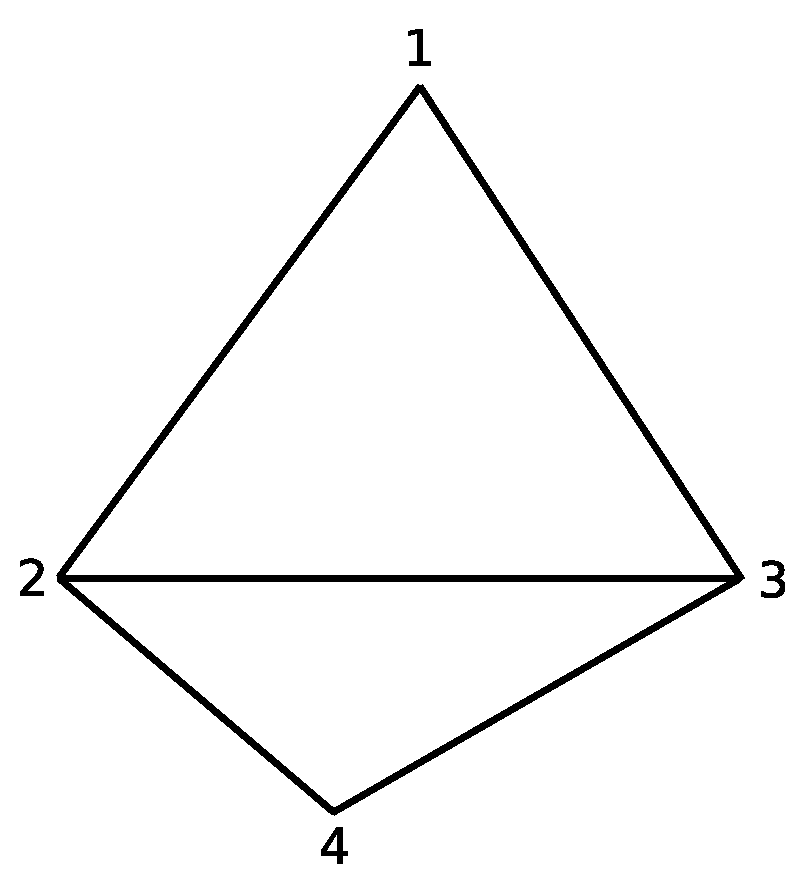
\includegraphics[width=4cm]{chap02/loop}
        \centerline{(a)图}\medskip
    \end{minipage}
  \begin{minipage}[b]{0.48\textwidth}
    \centering
    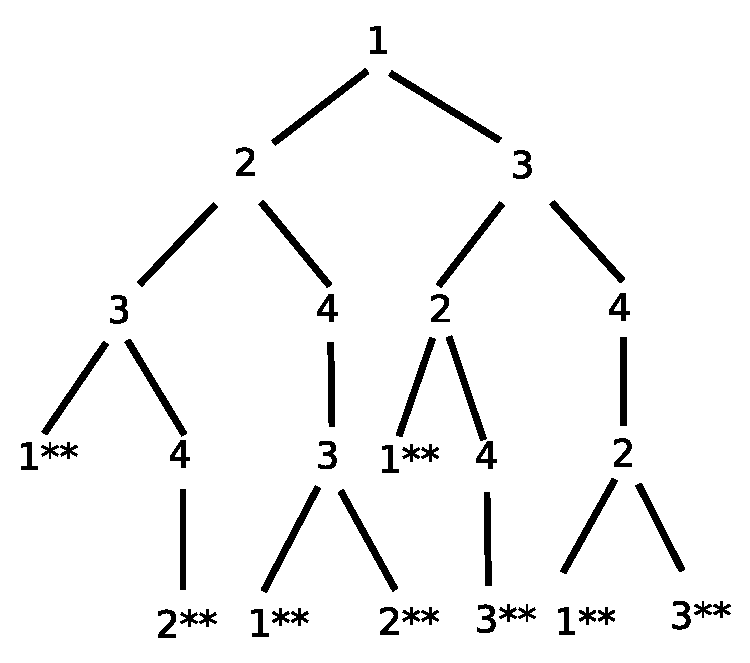
\includegraphics[width=5cm]{chap02/graph-old}
      \centerline{(b) 树}\medskip
  \end{minipage}
\caption{图与迭代环计数算法转化树}
\label{fig:graph-tree}
\end{figure}

由此可知,迭代环计数算法能够检测到图中的所有环,不仅包括最小环,还存在由最小环形成的大环。在图像中,我们感兴趣的是提取图像中的最小环结构。并且当图像中的环结构较多,点边关系错综复杂时,深度优先算法的搜索路径往往容易变得冗长,且迭代环计数算法的搜索路径容易重复,从而增加算法复杂性。

基于此,我们提出了基于广度优先检索策略的环结构检测算法,使得树结构更加简单,从而减小算法的复杂性。算法思想同样是把图变换成一颗树,但是基于广度优先算法,并且增加了对于兄弟结点的考虑,从而降低算法的复杂性,其主要步骤为:
\begin{enumerate}
\item 初始化一个结点作为树的根。
\item 找到与这个结点相邻的所有结点,并把他们作为根的子结点,放入树的第二层。相邻的点可以通过点边邻接矩阵得到,因为它列出了与某一点相邻的所有的结点。
\item 判断当前层是否有相邻的兄弟结点或相同的结点,若有,则说明有环形成。回到上一层,找到其相同的父结点或相邻的不同的父结点,若没有找到,则继续回到上一层,直到找到为止,那么,搜索路径上的点就可以组成环。
\item 继续检测与当前层的结点相连的除父结点及兄弟结点以外的其他结点并放入树的下一层。然后转入第三步,直到所有的点边关系遍历结束。
\end{enumerate}
经过以上步骤,所有三点、四点、五点环将被检测到。如图\ref{fig:cycle-tree}(a)是一个图的例子,图中有一个三点环、一个四点环、一个五点环。通过我们的环结构检测算法,这三个环要被准确无误的检测出来。首先确定$v_1$为初始点,即树的根。通过点边关系可得,与之相邻的点分别为$v_2, v_5, v_6, v_8$,于是,这四个点将被当作根的子结点放入树的第二层。判断这四个点是否有相邻点,发现$v_5, v_6$是相邻的,那么$v_5, v_6$及其相同的父结点$v_1$形成一个三点环,继续寻找这四个点的相邻点(除父结点及兄弟结点以外),放入树的第三层。判断这些点有没有相邻点或相同点。通过点边关系矩阵发现$v_3,v_4$是相邻点,那么$v_3,v_4$与其父结点$v_2,v_5$及其父结点的相同父结点$v_1$形成五点环,同理,$v_{1}v_{6}v_{7}v_{8}$组成四点环。至此,所有的搜索都已完成,即共找到三个环,$v_{1}v_{5}v_{6}$组成三点环,$v_{1}v_{6}v_{7}v_{8}$组成四点环,$v_{1}v_{2}v_{3}v_{4}v_{5}$组成五点环。

\begin{figure}
\centering
  \begin{minipage}[b]{1\textwidth} 
      \centering 
       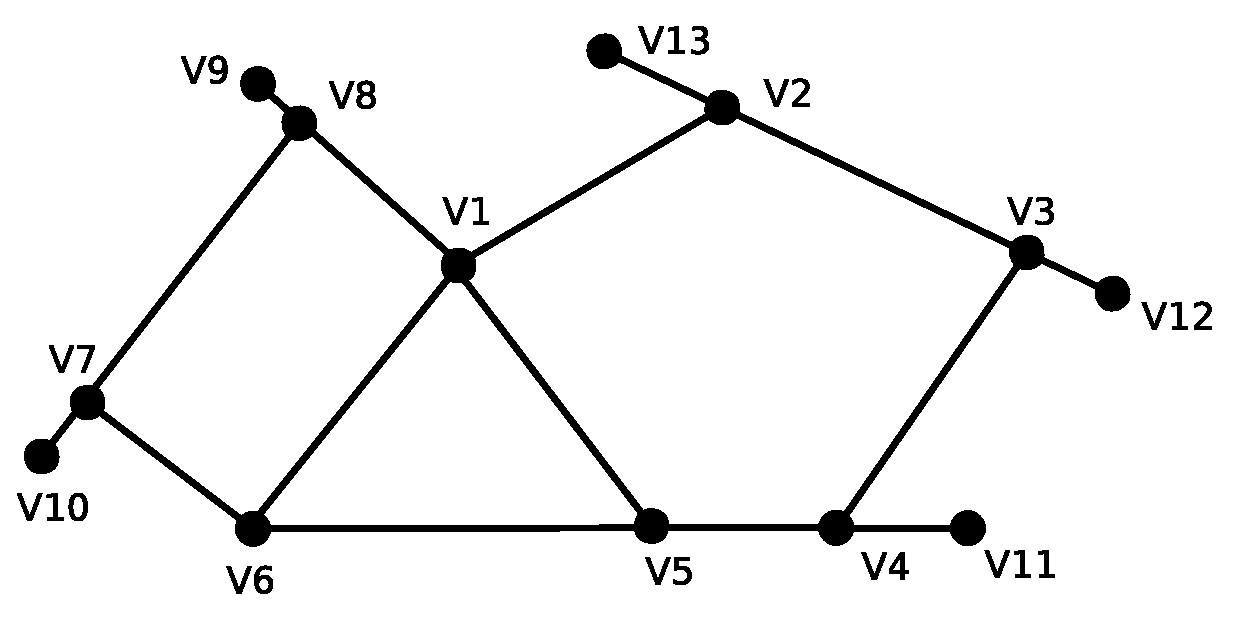
\includegraphics[width=7cm]{chap02/graph2}
       \centerline{(a)}\medskip
    \end{minipage}
  \begin{minipage}[b]{1\textwidth}
    \centering
    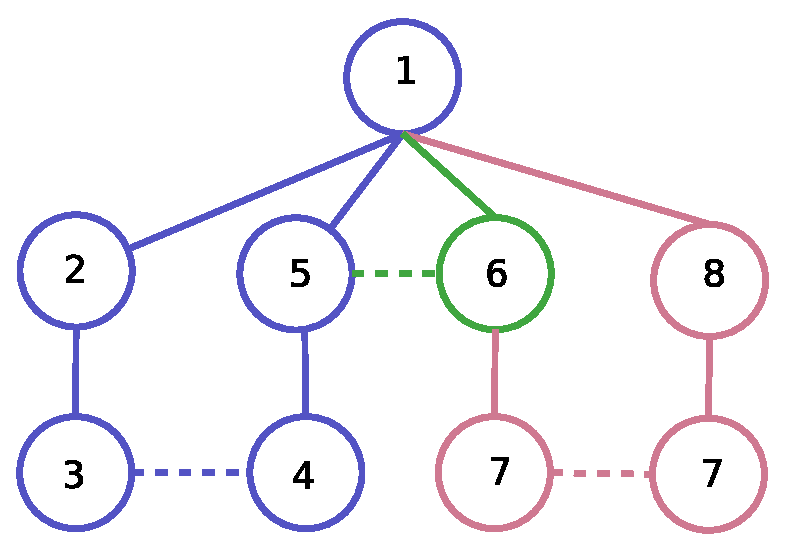
\includegraphics[width=6cm]{chap02/tree}
    \centerline{(b)}\medskip
  \end{minipage}
\caption{图与搜索树}
\label{fig:cycle-tree}
\end{figure}

通过我们提出的环结构检测算法算法,图\ref{fig:graph-tree}(a)可以转化为图\ref{fig:simple-tree}中的树,由此可以看到,相比图\ref{fig:graph-tree}(b)中的树,图\ref{fig:simple-tree}更加的简单,搜索路径不会重复,算法更加高效。

\begin{figure}
\centering
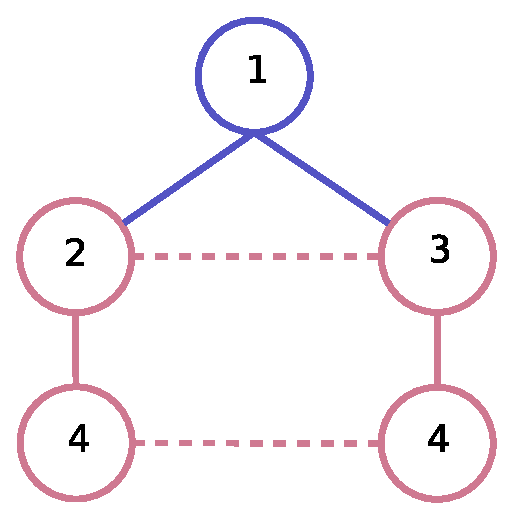
\includegraphics[width=0.3\textwidth]{chap02/simple-graph}
\caption{图\ref{fig:graph-tree}(a)的搜索树}
\label{fig:simple-tree}
\end{figure}


\section{环结构描述}
\label{}
环之所以能用在图像识别与匹配领域,是因为它是稳定的显著的特性。而它的稳定性与显著性则体现在用来描述环结构的特征向量上。

一个环结构是由一系列分叉点与连接这些分叉点之间的线组成。我们用分支角度与分支长度来描述环结构。以任意分叉点$v_i(x_0, y_0)$为中心,构造一个$7 \times 7$的邻域。记录分支与邻域边缘24个像素相交点的坐标,假设其坐标值为$x_j, y_j, j=1, 2, \ldots$。则分支方向为:
\begin{align}
\beta_j = arctan\frac{dy}{dx}, dy = y_j - y_0, dx = x_j - x_0 
\end{align}

由于arctan的取值范围为$-90^{\circ} \sim 90^{\circ}$,故还需保证求出的角度大于0。即
\begin{align}
\alpha_j = \left\{ \begin{array}{ll}
\beta_j & \textrm{$dy \geq 0$, $dx \geq 0$} \\
\beta_j + 180^{\circ} & \textrm{$dy \geq 0$, $dx \leq 0$ 或 $dy \leq 0$, $dx \geq 0$}\\
\beta_j + 360^{\circ} & \textrm{$dy \leq 0, dx \leq 0$}
\end{array} \right.
\end{align}
邻域边缘24个像素把$360^{\circ}$分成了24个离散值,每个相邻的分支角度相差$15^{\circ}$。每个角度以水平线为基准,故分叉点之间的角度值可通过式\ref{eq:Angle}计算:
\begin{align}
\theta_i = \alpha_{i+1} - \alpha_i, \qquad
\theta_i = \left\{ \begin{array}{ll}
\theta_i + 360^{\circ} & \theta_i \le 0 \\
\theta_i & \theta_i \geq 0
\end{array} \right.
\label{eq:Angle}
\end{align}
如图\ref{fig:calculate-angles},以三分叉点为中心划定一个$7\times7$邻域,邻域的边缘24个像素把$360^{\circ}$分为24个方向的角度,分别为$15^{\circ}, 30^{\circ},45^{\circ}, \ldots, 360^{\circ}$。在这个邻域的边缘24个像素中,像素值为1的像素以水平线为基准与中心像素形成分支角度,图\ref{fig:calculate-angles}中,共形成3个角度,即$45^{\circ}, 150^{\circ},270^{\circ}$,则分支之间的角度为$105^{\circ}, 120^{\circ}, 135^{\circ}$。

\begin{figure}[H]
\centering
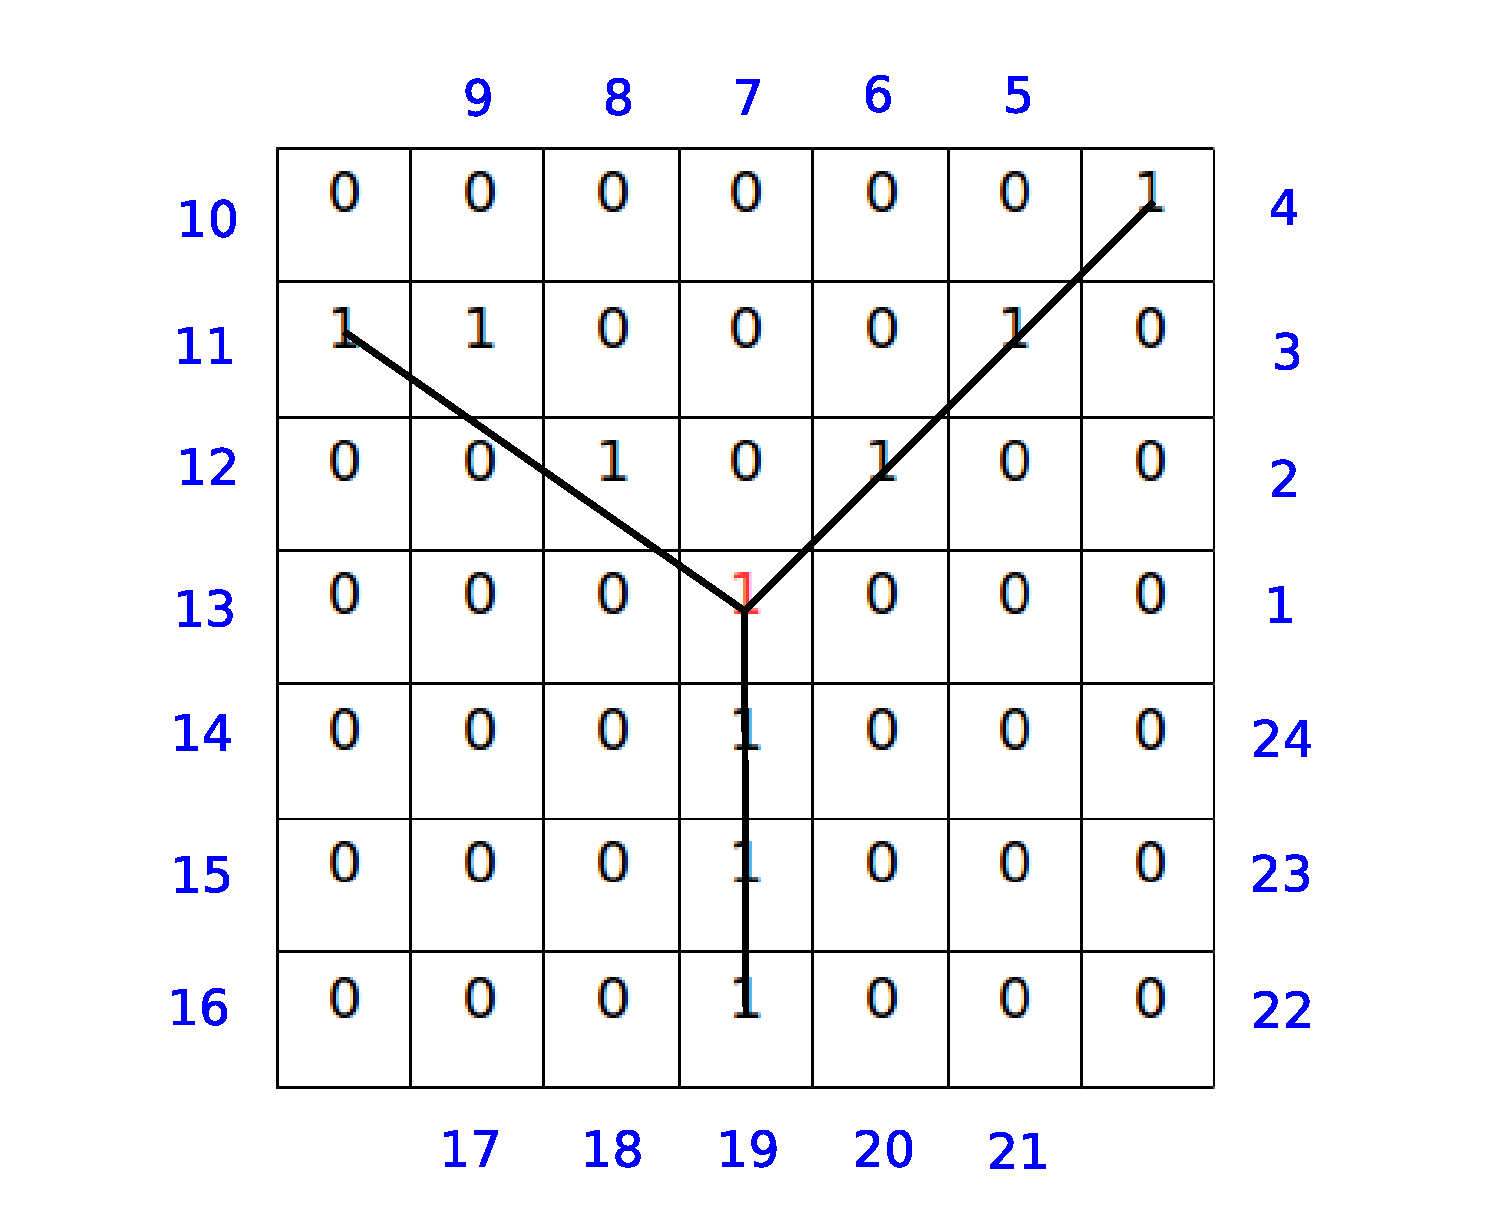
\includegraphics[width=0.5\textwidth]{chap02/7-7}
\caption{分支角度计算}
\label{fig:calculate-angles}
\end{figure}

分叉点之间的分支长度为分叉点之间的欧式距离,即:
\begin{align}
L = \sqrt{(y_j - y_0)^2 + (x_j - x_0)^2}, j = 1, 2, \ldots
\end{align}

归一化属于数字信号处理范畴,即将有量纲的表达式,经过变换,转换为无量纲的表达式,成为标量。它是简化计算,缩小量值的有效办法。而对于环结构特征,通过归一化,能使在减少计算量的基础上,使环结构特征具有平移、旋转及尺度不变性。图\ref{fig:description}给出了四点环结构示意图,角度归一化、长度归一化及最终产生的特征向量可分别用式\ref{eq:angle}、式\ref{eq:length}及式\ref{eq:vector}表示。$L_{1} \sim L_{4}$,$\theta_{1} \sim \theta_{14}$,$\theta_{15} \sim \theta_{18}$ 分别代表分支长度、分支角度及分叉点之间的角度。

\begin{figure}[H]
\centering
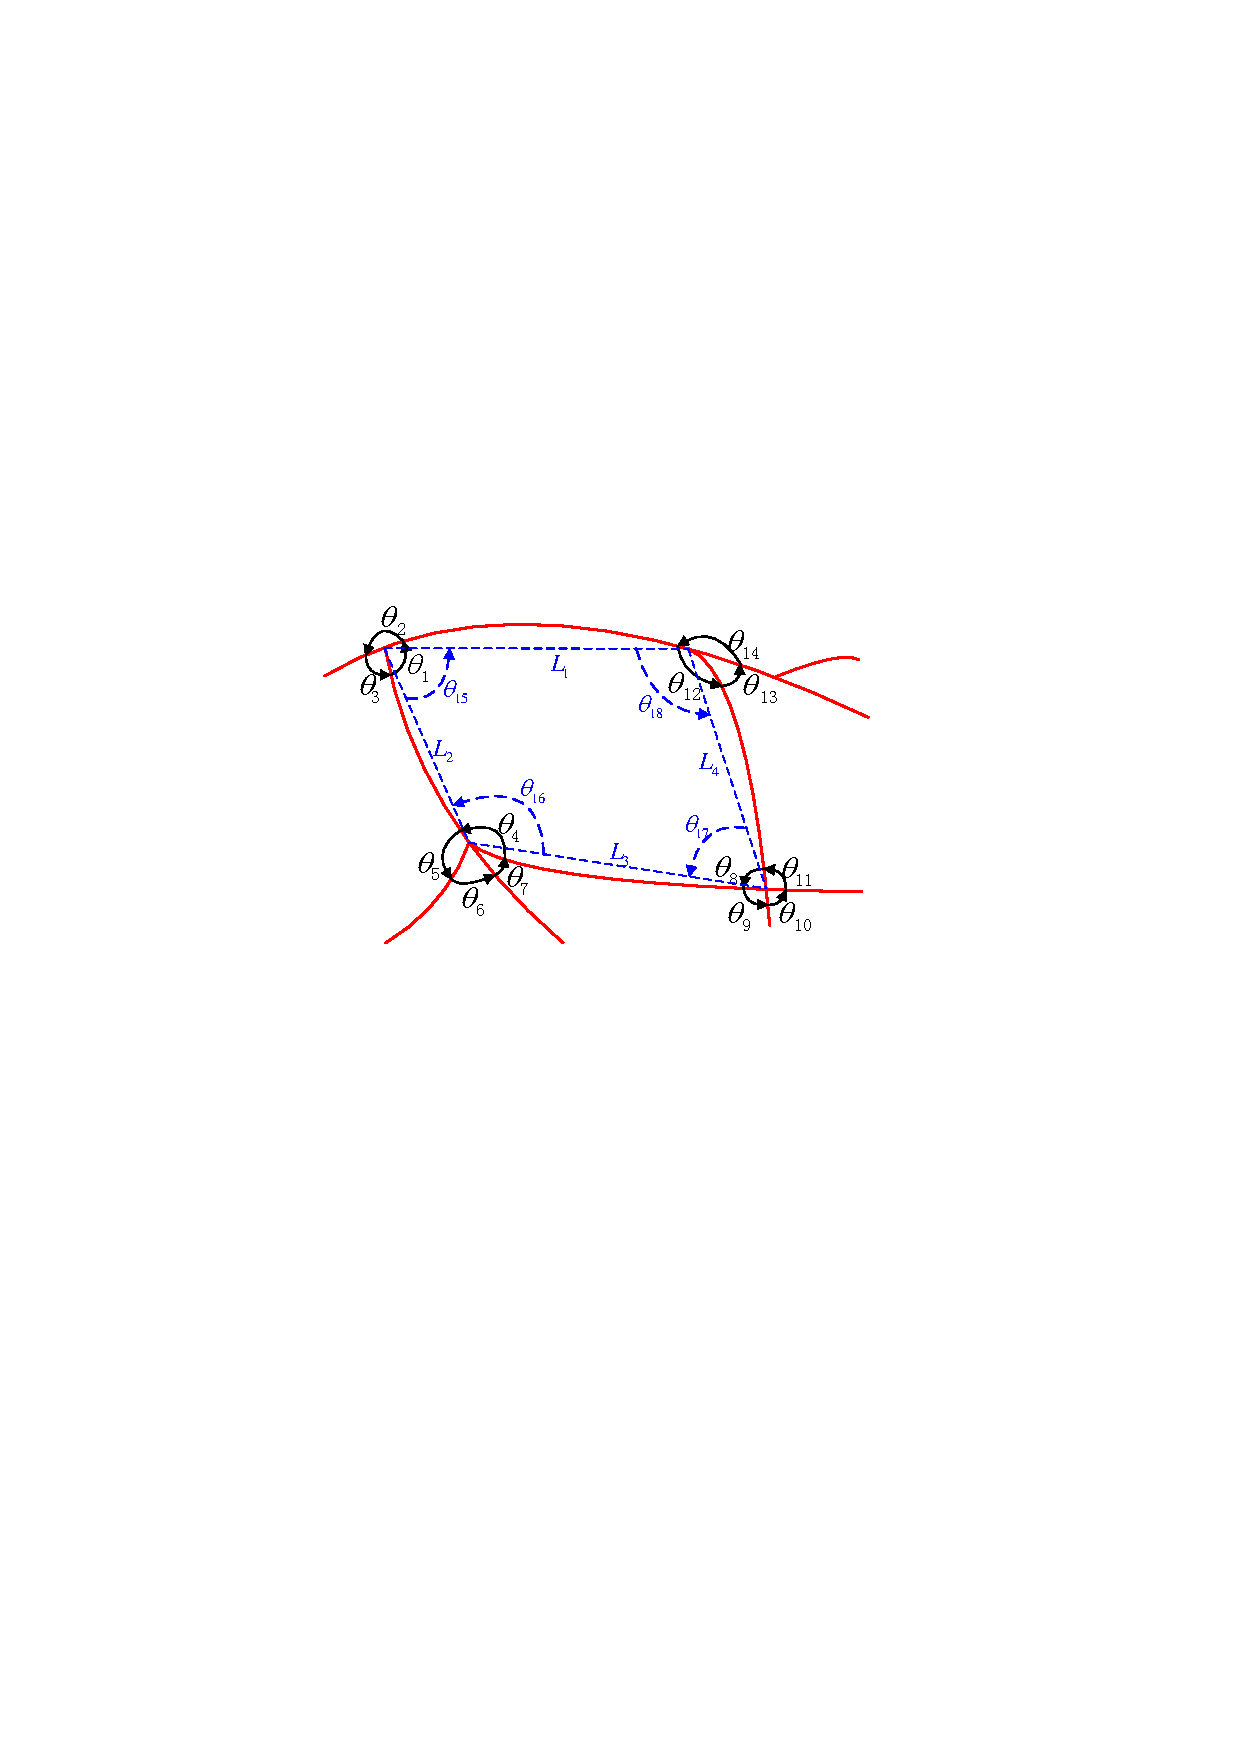
\includegraphics[width=0.4\textwidth]{chap02/description.pdf}
\caption{环结构描述}
\label{fig:description}
\end{figure}
\begin{align}
L_{iNorm}&=\frac{L_i}{\sum{L}}\label{eq:length}\\
\theta_{jNorm}&=\frac{\theta_j}{360^\circ}\label{eq:angle}
\end{align}
\begin{multline}
\tilde{v}=\{\textrm{角度,长度}\}=\{L_{1},L_{2},L_{3},L_{4},\theta_{1},\theta_{2},\theta_{3},\mathbf{0},\theta_{4},\\\theta_{5},\theta_{6},\theta_{7},\theta_{8},\theta_{9},\theta_{10},\theta_{11},\theta_{12},\theta_{13},\theta_{14},\mathbf{0},\theta_{15},\theta_{16},\theta_{17},\theta_{18}\}
\label{eq:vector}
\end{multline}

值得注意的是,组成环的分叉点个数不一样,并且每个分叉点的分叉角度也不同,这就导致了不同类型的环有不同长度的特征向量。为了便于识别和配准的需要,我们可根据实际情况设定一个角度个数标准,比如说,若设置4个分支角度为标准,那么小于4个角度的分叉应用0来补齐,这样就保证同种类型的环的特征向量的长度是相同的。这样,当用来做配准或识别时,就可匹配同种类型的环的特征向量来达到目的。

\section{本章小节}
\label{}

本章介绍了环结构特征的定义、特点及应用,阐述了从图像中检测环的主要步骤:检测分叉点及其连接关系、滤除无效分叉点、检测环结构,并重点介绍了我们提出的环结构检测算法。同时,结合环结构的特点,给出了特征描述的方法。通过把环结构特征表示成为特征向量,就能为下一步的配准、识别奠定基础。

%
%
% %%% 其它部分
% \backmatter
% % 插图索引
% \listoffigures
% % 表格索引
% \listoftables
% % 公式索引
% \listofequations
%
%
% % 参考文献
% \bibliographystyle{thubib}
% \bibliography{ref/refs}
%
%
% % 致谢
% %%% Local Variables:
%%% mode: latex
%%% TeX-master: "../main"
%%% End:

\begin{ack}
硕士研究生生涯即将结束,在这三年的生活里,我得到了许多人的关心和帮助,在此表示最真诚的感谢!

衷心感谢我的导师郑海永老师三年来对我的学习和生活无微不至的关怀!导师专业的科研态度、追求卓越的理念,缜密的思维是我终生学习的榜样,郑老师针对我的行为处事方法,思维习惯提出的宝贵的意见,使我充分地认识到自己的缺点与不足,这些不足将时刻提醒自己要改变,以求遇见更好的自己。感谢师母冯丽颖的支持和鼓励,不断提供正能量督促我们前进。感谢姬光荣老师的关怀和鼓励。在此各位致以崇高的敬意。

感谢各位实验室兄弟姐妹,因为有你们,我度过了一段开心难忘的研究生生活。感谢我的师妹邱欣欣和师弟高远宁同学对我的科研课题给予了很多的支持和帮助。感谢赵红苗陪我一起走完了这段旅程。

感谢我的家人,我走过的每一步都凝聚着你们的心血,你们是我的稳固后方和支持我不断前进的力量源泉!感谢我的男朋友在我失落时给予鼓励。

感谢国家自然科学基金项目``基于视觉注意结合生物形态特征的海洋浮游植物显微图像分析"(编号:61301240)与``基于形态特征的中国海常见有害赤潮藻显微图像识别''(编号:61271406)资助,感谢中国海洋大学海洋海洋生命学院王扬帆老师提供的帮助。

最后,感谢所有关心和帮助过我的人,祝愿你们幸福安康!
\end{ack}

%
% % 附录
% \begin{appendix}
% %%% Local Variables: 
%%% mode: latex
%%% TeX-master: "../main"
%%% End: 

\chapter{外文资料原文}
\label{cha:engorg}
As one of the most widely used techniques in operations research, {\em
  mathematical programming} is defined as a means of maximizing a quantity known
as {\em objective function}, subject to a set of constraints represented by
equations and inequalities. Some known subtopics of mathematical programming are
linear programming, nonlinear programming, multiobjective programming, goal
programming, dynamic programming, and multilevel programming$^{[1]}$.

It is impossible to cover in a single chapter every concept of mathematical
programming. This chapter introduces only the basic concepts and techniques of
mathematical programming such that readers gain an understanding of them
throughout the book$^{[2,3]}$.


\section{Single-Objective Programming}
The general form of single-objective programming (SOP) is written
as follows,
\begin{equation}\tag*{(123)} % 如果附录中的公式不想让它出现在公式索引中,那就请
                             % 用 \tag*{xxxx}
\left\{\begin{array}{l}
\max \,\,f(x)\\[0.1 cm]
\mbox{subject to:} \\ [0.1 cm]
\qquad g_j(x)\le 0,\quad j=1,2,\cdots,p
\end{array}\right.
\end{equation}
which maximizes a real-valued function $f$ of
$x=(x_1,x_2,\cdots,x_n)$ subject to a set of constraints.

\newtheorem{mpdef}{Definition}[chapter]
\begin{mpdef}
In SOP, we call $x$ a decision vector, and
$x_1,x_2,\cdots,x_n$ decision variables. The function
$f$ is called the objective function. The set
\begin{equation}\tag*{(456)} % 这里同理,其它不再一一指定。
S=\left\{x\in\Re^n\bigm|g_j(x)\le 0,\,j=1,2,\cdots,p\right\}
\end{equation}
is called the feasible set. An element $x$ in $S$ is called a
feasible solution.
\end{mpdef}

\newtheorem{mpdefop}[mpdef]{Definition}
\begin{mpdefop}
A feasible solution $x^*$ is called the optimal
solution of SOP if and only if
\begin{equation}
f(x^*)\ge f(x)
\end{equation}
for any feasible solution $x$.
\end{mpdefop}

One of the outstanding contributions to mathematical programming was known as
the Kuhn-Tucker conditions\ref{eq:ktc}. In order to introduce them, let us give
some definitions. An inequality constraint $g_j(x)\le 0$ is said to be active at
a point $x^*$ if $g_j(x^*)=0$. A point $x^*$ satisfying $g_j(x^*)\le 0$ is said
to be regular if the gradient vectors $\nabla g_j(x)$ of all active constraints
are linearly independent.

Let $x^*$ be a regular point of the constraints of SOP and assume that all the
functions $f(x)$ and $g_j(x),j=1,2,\cdots,p$ are differentiable. If $x^*$ is a
local optimal solution, then there exist Lagrange multipliers
$\lambda_j,j=1,2,\cdots,p$ such that the following Kuhn-Tucker conditions hold,
\begin{equation}
\label{eq:ktc}
\left\{\begin{array}{l}
    \nabla f(x^*)-\sum\limits_{j=1}^p\lambda_j\nabla g_j(x^*)=0\\[0.3cm]
    \lambda_jg_j(x^*)=0,\quad j=1,2,\cdots,p\\[0.2cm]
    \lambda_j\ge 0,\quad j=1,2,\cdots,p.
\end{array}\right.
\end{equation}
If all the functions $f(x)$ and $g_j(x),j=1,2,\cdots,p$ are convex and
differentiable, and the point $x^*$ satisfies the Kuhn-Tucker conditions
(\ref{eq:ktc}), then it has been proved that the point $x^*$ is a global optimal
solution of SOP.

\subsection{Linear Programming} 
\label{sec:lp}

If the functions $f(x),g_j(x),j=1,2,\cdots,p$ are all linear, then SOP is called
a {\em linear programming}.

The feasible set of linear is always convex. A point $x$ is called an extreme
point of convex set $S$ if $x\in S$ and $x$ cannot be expressed as a convex
combination of two points in $S$. It has been shown that the optimal solution to
linear programming corresponds to an extreme point of its feasible set provided
that the feasible set $S$ is bounded. This fact is the basis of the {\em simplex
  algorithm} which was developed by Dantzig as a very efficient method for
solving linear programming.
\begin{table}[ht]
\centering
  \centering
  \caption*{Table~1\hskip1em This is an example for manually numbered table, which
    would not appear in the list of tables}
  \label{tab:badtabular2}
  \begin{tabular}[c]{|c|m{0.8in}|c|c|c|c|c|}\hline
    \multicolumn{2}{|c|}{Network Topology} & \# of nodes & 
    \multicolumn{3}{c|}{\# of clients} & Server \\\hline
    GT-ITM & Waxman Transit-Stub & 600 &
    \multirow{2}{2em}{2\%}& 
    \multirow{2}{2em}{10\%}& 
    \multirow{2}{2em}{50\%}& 
    \multirow{2}{1.2in}{Max. Connectivity}\\\cline{1-3}
    \multicolumn{2}{|c|}{Inet-2.1} & 6000 & & & &\\\hline
    \multirow{2}{1in}{Xue} & Rui  & Ni &\multicolumn{4}{c|}{\multirow{2}*{\thuthesis}}\\\cline{2-3}
    & \multicolumn{2}{c|}{ABCDEF} &\multicolumn{4}{c|}{} \\\hline
\end{tabular}  
\end{table}

Roughly speaking, the simplex algorithm examines only the extreme points of the
feasible set, rather than all feasible points. At first, the simplex algorithm
selects an extreme point as the initial point. The successive extreme point is
selected so as to improve the objective function value. The procedure is
repeated until no improvement in objective function value can be made. The last
extreme point is the optimal solution.

\subsection{Nonlinear Programming}

If at least one of the functions $f(x),g_j(x),j=1,2,\cdots,p$ is nonlinear, then
SOP is called a {\em nonlinear programming}.

A large number of classical optimization methods have been developed to treat
special-structural nonlinear programming based on the mathematical theory
concerned with analyzing the structure of problems.
\begin{figure}[h]
  \centering
  \includegraphics[clip]{thu-lib-logo}
  \caption*{Figure~1\hskip1em This is an example for manually numbered figure,
    which would not appear in the list of figures}
  \label{tab:badfigure2}    
\end{figure}

Now we consider a nonlinear programming which is confronted solely with
maximizing a real-valued function with domain $\Re^n$.  Whether derivatives are
available or not, the usual strategy is first to select a point in $\Re^n$ which
is thought to be the most likely place where the maximum exists. If there is no
information available on which to base such a selection, a point is chosen at
random. From this first point an attempt is made to construct a sequence of
points, each of which yields an improved objective function value over its
predecessor. The next point to be added to the sequence is chosen by analyzing
the behavior of the function at the previous points. This construction continues
until some termination criterion is met. Methods based upon this strategy are
called {\em ascent methods}, which can be classified as {\em direct methods},
{\em gradient methods}, and {\em Hessian methods} according to the information
about the behavior of objective function $f$. Direct methods require only that
the function can be evaluated at each point. Gradient methods require the
evaluation of first derivatives of $f$. Hessian methods require the evaluation
of second derivatives. In fact, there is no superior method for all
problems. The efficiency of a method is very much dependent upon the objective
function.

\subsection{Integer Programming}

{\em Integer programming} is a special mathematical programming in which all of
the variables are assumed to be only integer values. When there are not only
integer variables but also conventional continuous variables, we call it {\em
  mixed integer programming}. If all the variables are assumed either 0 or 1,
then the problem is termed a {\em zero-one programming}. Although integer
programming can be solved by an {\em exhaustive enumeration} theoretically, it
is impractical to solve realistically sized integer programming problems. The
most successful algorithm so far found to solve integer programming is called
the {\em branch-and-bound enumeration} developed by Balas (1965) and Dakin
(1965). The other technique to integer programming is the {\em cutting plane
  method} developed by Gomory (1959).

\hfill\textit{Uncertain Programming\/}\quad(\textsl{BaoDing Liu, 2006.2})

\section*{References}
\noindent{\itshape NOTE: these references are only for demonstration, they are
  not real citations in the original text.}

\begin{enumerate}[{$[$}1{$]$}]
\item Donald E. Knuth. The \TeX book. Addison-Wesley, 1984. ISBN: 0-201-13448-9
\item Paul W. Abrahams, Karl Berry and Kathryn A. Hargreaves. \TeX\ for the
  Impatient. Addison-Wesley, 1990. ISBN: 0-201-51375-7
\item David Salomon. The advanced \TeX book.  New York : Springer, 1995. ISBN:0-387-94556-3
\end{enumerate}

\chapter{外文资料的调研阅读报告或书面翻译}
\section{单目标规划}
北冥有鱼,其名为鲲。鲲之大,不知其几千里也。化而为鸟,其名为鹏。鹏之背,不知其几
千里也。怒而飞,其翼若垂天之云。是鸟也,海运则将徙于南冥。南冥者,天池也。 
\begin{equation}\tag*{(123)}
 p(y|\mathbf{x}) = \frac{p(\mathbf{x},y)}{p(\mathbf{x})}=
\frac{p(\mathbf{x}|y)p(y)}{p(\mathbf{x})}
\end{equation}

吾生也有涯,而知也无涯。以有涯随无涯,殆已!已而为知者,殆而已矣!为善无近名,为
恶无近刑,缘督以为经,可以保身,可以全生,可以养亲,可以尽年。

\subsection{线性规划}
庖丁为文惠君解牛,手之所触,肩之所倚,足之所履,膝之所倚,砉然响然,奏刀騞然,莫
不中音,合于桑林之舞,乃中经首之会。
\begin{table}[ht]
\centering
  \centering
  \caption*{表~1\hskip1em 这是手动编号但不出现在索引中的一个表格例子}
  \label{tab:badtabular3}
  \begin{tabular}[c]{|c|m{0.8in}|c|c|c|c|c|}\hline
    \multicolumn{2}{|c|}{Network Topology} & \# of nodes & 
    \multicolumn{3}{c|}{\# of clients} & Server \\\hline
    GT-ITM & Waxman Transit-Stub & 600 &
    \multirow{2}{2em}{2\%}& 
    \multirow{2}{2em}{10\%}& 
    \multirow{2}{2em}{50\%}& 
    \multirow{2}{1.2in}{Max. Connectivity}\\\cline{1-3}
    \multicolumn{2}{|c|}{Inet-2.1} & 6000 & & & &\\\hline
    \multirow{2}{1in}{Xue} & Rui  & Ni &\multicolumn{4}{c|}{\multirow{2}*{\thuthesis}}\\\cline{2-3}
    & \multicolumn{2}{c|}{ABCDEF} &\multicolumn{4}{c|}{} \\\hline
\end{tabular}  
\end{table}

文惠君曰:“嘻,善哉!技盖至此乎?”庖丁释刀对曰:“臣之所好者道也,进乎技矣。始臣之
解牛之时,所见无非全牛者;三年之后,未尝见全牛也;方今之时,臣以神遇而不以目视,
官知止而神欲行。依乎天理,批大郤,导大窾,因其固然。技经肯綮之未尝,而况大坬乎!
良庖岁更刀,割也;族庖月更刀,折也;今臣之刀十九年矣,所解数千牛矣,而刀刃若新发
于硎。彼节者有间而刀刃者无厚,以无厚入有间,恢恢乎其于游刃必有余地矣。是以十九年
而刀刃若新发于硎。虽然,每至于族,吾见其难为,怵然为戒,视为止,行为迟,动刀甚微,
謋然已解,如土委地。提刀而立,为之而四顾,为之踌躇满志,善刀而藏之。”

文惠君曰:“善哉!吾闻庖丁之言,得养生焉。”


\subsection{非线性规划}
孔子与柳下季为友,柳下季之弟名曰盗跖。盗跖从卒九千人,横行天下,侵暴诸侯。穴室枢
户,驱人牛马,取人妇女。贪得忘亲,不顾父母兄弟,不祭先祖。所过之邑,大国守城,小
国入保,万民苦之。孔子谓柳下季曰:“夫为人父者,必能诏其子;为人兄者,必能教其弟。
若父不能诏其子,兄不能教其弟,则无贵父子兄弟之亲矣。今先生,世之才士也,弟为盗
跖,为天下害,而弗能教也,丘窃为先生羞之。丘请为先生往说之。”
\begin{figure}[h]
  \centering
  \includegraphics{hello}
  \caption*{图~1\hskip1em 这是手动编号但不出现索引中的图片的例子}
  \label{tab:badfigure3}    
\end{figure}

柳下季曰:“先生言为人父者必能诏其子,为人兄者必能教其弟,若子不听父之诏,弟不受
兄之教,虽今先生之辩,将奈之何哉?且跖之为人也,心如涌泉,意如飘风,强足以距敌,
辩足以饰非。顺其心则喜,逆其心则怒,易辱人以言。先生必无往。”

孔子不听,颜回为驭,子贡为右,往见盗跖。

\subsection{整数规划}
盗跖乃方休卒徒大山之阳,脍人肝而餔之。孔子下车而前,见谒者曰:“鲁人孔丘,闻将军
高义,敬再拜谒者。”谒者入通。盗跖闻之大怒,目如明星,发上指冠,曰:“此夫鲁国之
巧伪人孔丘非邪?为我告之:尔作言造语,妄称文、武,冠枝木之冠,带死牛之胁,多辞缪
说,不耕而食,不织而衣,摇唇鼓舌,擅生是非,以迷天下之主,使天下学士不反其本,妄
作孝弟,而侥幸于封侯富贵者也。子之罪大极重,疾走归!不然,我将以子肝益昼餔之膳。”


\chapter{其它附录}
前面两个附录主要是给本科生做例子。其它附录的内容可以放到这里,当然如果你愿意,可
以把这部分也放到独立的文件中,然后将其 \verb|\input| 到主文件中。
% \end{appendix}
%
% % 个人简历
% \begin{resume}

  \resumeitem{个人简历}

  xxxx 年 xx 月 xx 日出生于 xx 省 xx 县。
  
  xxxx 年 9 月考入 xx 大学 xx 系 xx 专业,xxxx 年 7 月本科毕业并获得 xx 学士学位。
  
  xxxx 年 9 月免试进入 xx 大学 xx 系攻读 xx 学位至今。

  \resumeitem{发表的学术论文} % 发表的和录用的合在一起

  \begin{enumerate}[{[}1{]}]
  \item Yang Y, Ren T L, Zhang L T, et al. Miniature microphone with silicon-
    based ferroelectric thin films. Integrated Ferroelectrics, 2003,
    52:229-235. (SCI 收录, 检索号:758FZ.)
  \item 杨轶, 张宁欣, 任天令, 等. 硅基铁电微声学器件中薄膜残余应力的研究. 中国机
    械工程, 2005, 16(14):1289-1291. (EI 收录, 检索号:0534931 2907.)
  \item 杨轶, 张宁欣, 任天令, 等. 集成铁电器件中的关键工艺研究. 仪器仪表学报,
    2003, 24(S4):192-193. (EI 源刊.)
  \item Yang Y, Ren T L, Zhu Y P, et al. PMUTs for handwriting recognition. In
    press. (已被 Integrated Ferroelectrics 录用. SCI 源刊.)
  \item Wu X M, Yang Y, Cai J, et al. Measurements of ferroelectric MEMS
    microphones. Integrated Ferroelectrics, 2005, 69:417-429. (SCI 收录, 检索号
    :896KM.)
  \item 贾泽, 杨轶, 陈兢, 等. 用于压电和电容微麦克风的体硅腐蚀相关研究. 压电与声
    光, 2006, 28(1):117-119. (EI 收录, 检索号:06129773469.)
  \item 伍晓明, 杨轶, 张宁欣, 等. 基于MEMS技术的集成铁电硅微麦克风. 中国集成电路, 
    2003, 53:59-61.
  \end{enumerate}

  \resumeitem{研究成果} % 有就写,没有就删除
  \begin{enumerate}[{[}1{]}]
  \item 任天令, 杨轶, 朱一平, 等. 硅基铁电微声学传感器畴极化区域控制和电极连接的
    方法: 中国, CN1602118A. (中国专利公开号.)
  \item Ren T L, Yang Y, Zhu Y P, et al. Piezoelectric micro acoustic sensor
    based on ferroelectric materials: USA, No.11/215, 102. (美国发明专利申请号.)
  \end{enumerate}
\end{resume}

%
% \end{document}
% \end{example}
%
% \subsection{选项}
% \label{sec:option}
% 本模板提供了一些选项以方便使用:
% \begin{description}
% \item[bachelor]
%   如果写本科论文将此选项打开。
%   \begin{example}
% \documentclass[bachelor]{thuthesis}
%   \end{example}
%
% \item[master]
%   如果写硕士论文将此选项打开。
%   \begin{example}
% \documentclass[master]{thuthesis}
%   \end{example}
%
% \item[doctor]
%   如果写博士论文将此选项打开。
%   \begin{example}
% \documentclass[doctor]{thuthesis}
%   \end{example}
%
% \item[postdoctor]
%   如果写博士博士后出站报告将此选项打开。
%   \begin{example}
% \documentclass[postdoctor]{thuthesis}
%   \end{example}
%
% \item[secret]
%   涉秘论文开关。配合另外两个命令 \cs{secretlevel} 和 \cs{secretyear} 分别用来指
%   定保密级别和时间。二者默认分别为\textbf{秘密}和当前年份。可以通
%   过:|\secretlevel{绝密}| 和 |\secretyear}{1984}| 修改。
%   \begin{example}
% \documentclass[bachelor, secret]{thuthesis}
%   \end{example}
%
% \changes{v3.0}{2007/05/12}{不用专门为本科论文生成\textbf{提交}版本了。}
%
% \item[openany, openright]
%   正规出版物的章节出现在奇数页,也就是右手边的页面,这就是 \option{openright},
%   也是 \thuthesis\ 的默认选项。在这种情况下,如果前一章的最后一页也是奇数,那么
%   模板会自动生成一个纯粹的空白页,很多人不是很习惯这种方式,而且学校的格式似乎
%   更倾向于页面连续,那就是通常所说的 \option{openany}。{\fangsong 目前所有论文
%   都是 \option{openany}。}这两个选项不用专门设置,\thuthesis{} 会根据当前论文类
%   型自动选择。
%
% \item[winfonts, adobefonts, nofonts]
%   这些选项用来指导 \pkg{ctex} 宏包/文档类设置选用的中文字体。
%   \begin{itemize}
%   \item \option{winfonts} 指定使用中易的六款字体(Xe\TeX 下为四种)。
%   \item \option{adobefonts} 指定使用 Adobe 的四款免费中文字体。
%   \item \option{nofonts} 不提供可用的中文字体,由用户自行设定。
%   \end{itemize}
%
% \item[arial]
%   使用真正的 \option{arial} 字体。此选项会装载 \pkg{arial} 字体宏包,如果此宏包
%   不存在,就装
%   载 \pkg{Helvet}。\option{arialtoc} 和 \option{arialtitle} 不受
%   \texttt{arial} 的影响。因为一般的 \TeX{} 发行都没有 \pkg{arial} 字体,所以默
%   认采用 \pkg{Helvet},二者效果非常相似。如果一定要用 \pkg{arial} 字体,请参
%   看:\href{http://www.mail-archive.com/ctan-ann@dante.de/msg00627.html}{Arial
%   字体}。
%
% \item[arialtoc]
%   目录项(章目录项除外)中的英文是否用 \option{arial} 字体。本选项
%   和 \option{arialtitle} 都不用用户干预,模板根据当前论文类型自动设置。
%
% \item[arialtitle]
%   章节标题中英文是否用 \option{arial} 字体(默认打开)。
% \end{description}
%
% \subsection{字体配置}
% \label{sec:font-config}
% 正确配置中文字体是使用模板的第一步。模板调用 \pkg{ctex} 宏包,提供如下字体使用方式:
% \begin{itemize}
%   \item 基于传统 \pkg{CJK} 包,使用 latex、pdflatex 编译;
%   \item 基于 \pkg{xeCJK} 包,使用 xelatex 编译。
% \end{itemize}
%
% 第一种方式的字体配置比较繁琐,建议使用 \emph{donated@newsmth} 制作的中文字体包
% (自包含安装方法),请用户自行下载安装,此处不再赘述。本模板推荐使用第二种方法,
% 只要把所需字体放入系统字体文件夹(也可以指定自定义文件夹)即可。用户可以使
% 用 \option{winfonts},\option{adobefonts},\option{nofonts} 选项来选择可用的中
% 文字库,缺省为 \option{winfonts} 有效,使用中易字体。当使用 xelatex 编译
% 时,\option{winfonts} 只有中易的四款字体(宋体、黑体、楷书和仿宋)可用,而本科
% 生需要用到幼圆,另外 Linux 系统缺少上述字体,这些用户可以通过指
% 定 \option{nofonts} 选项,利用 \file{thufonts.def} 文件配置所需字体。使用中易
% 六种字体的配置如下:
% \begin{example}
% \ProvidesFile{thufonts.def}
% \setCJKmainfont[BoldFont={SimHei},ItalicFont={KaiTi}]{SimSun}
% \setCJKsansfont{SimHei}
% \setCJKmonofont{FangSong}
% \setCJKfamilyfont{zhsong}{SimSun}
% \setCJKfamilyfont{zhhei}{SimHei}
% \setCJKfamilyfont{zhkai}{KaiTi}
% \setCJKfamilyfont{zhfs}{FangSong}
% \setCJKfamilyfont{zhli}{LiSu}
% \setCJKfamilyfont{zhyou}{YouYuan}
% \newcommand*{\songti}{\CJKfamily{zhsong}} % 宋体
% \newcommand*{\heiti}{\CJKfamily{zhhei}}   % 黑体
% \newcommand*{\kaishu}{\CJKfamily{zhkai}}  % 楷书
% \newcommand*{\fangsong}{\CJKfamily{zhfs}} % 仿宋
% \newcommand*{\lishu}{\CJKfamily{zhli}}    % 隶书
% \newcommand*{\youyuan}{\CJKfamily{zhyou}} % 幼圆
% \end{example}
%
% 对 Windows XP 来说如下,|KaiTi| 需要替换为 |KaiTi_GB2312|,|FangSong| 需要替换
% 为 |FangSong_GB2312|。
%
% 宏包中包含了 \file{zhfonts.py} 脚本,为 Linux/Mac 用户提供一种交互式的方式从系
% 统中文字体中选择合适的六种字体,最终生成对应的 \file{thufonts.def}文件。要使用
% 它,只需在命令行输入该脚本的完整路径即可。
%
% 另外,用户也可以通过命令
% \begin{shell}
% $ fs-list :lang=zh > zhfonts.txt
% \end{shell}
% 得到系统中现有的中文字体列表,并相应替换上述配置。
%
% \subsection{命令}
% \label{sec:command}
% 模板中的命令分为两类:一是格式控制,二是内容替换。格式控制如字体、字号、字距和
% 行距。内容替换如姓名、院系、专业、致谢等等。其中内容替换命令居多,而且主要集中
% 在封面上,其中有以本科论文为最(比硕士和博士论文多了\textbf{综合论文训练任务书}一
% 页)。首先来看格式控制命令。
%
% \subsubsection{基本控制命令}
% \label{sec:basiccom}
%
% \myentry{字体}
% \DescribeMacro{\songti}
% \DescribeMacro{\fangsong}
% \DescribeMacro{\heiti}
% \DescribeMacro{\kaishu}
% \DescribeMacro{\lishu}
% \DescribeMacro{\youyuan}
% 等分别用来切换宋体、仿宋、黑体、楷体、隶书和幼圆字体。
%
% \begin{example}
% {\songti 乾:元,亨,利贞}
% {\fangsong 初九,潜龙勿用}
% {\heiti 九二,见龙在田,利见大人}
% {\kaishu 九三,君子终日乾乾,夕惕若,厉,无咎}
% {\lishu 九四,或跃在渊,无咎}
% {\heiti 九五,飞龙在天,利见大人}
% {\songti 上九,亢龙有悔}
% {\youyuan 用九,见群龙无首,吉}
% \end{example}
%
% \myentry{字号}
% \DescribeMacro{\chuhao}
% 等命令定义一组字体大小,分别为:
%
% \begin{center}
% \begin{tabular}{lllll}
% \hline
% |\chuhao|&|\xiaochu|&|\yihao|&|\xiaoyi| &\\
% |\erhao|&|\xiaoer|&|\sanhao|&|\xiaosan|&\\
% |\sihao|& |\banxiaosi|&|\xiaosi|&|\dawu|&|\wuhao|\\
% |\xiaowu|&|\liuhao|&|\xiaoliu|&|\qihao|& |\bahao|\\\hline
% \end{tabular}
% \end{center}
%
% 使用方法为:\cs{command}\oarg{num},其中 |command| 为字号命令,|num| 为行距。比
% 如 |\xiaosi[1.5]| 表示选择小四字体,行距 1.5 倍。写作指南要求表格中的字体
% 是 \cs{dawu},模板已经设置好了。
%
% \begin{example}
% {\erhao 二号 \sanhao 三号 \sihao 四号  \qihao 七号}
% \end{example}
%
% \myentry{密级}
% \DescribeMacro{\secretlevel}
% \DescribeMacro{\secretyear}
% 定义秘密级别和年限:
%   \begin{example}
% \secretyear{5}
% \secretlevel{内部}
%   \end{example}
%
% \myentry{引用方式}
% \DescribeMacro{\onlinecite}

% 学校要求的参考文献引用有两种模式:(1)上标模式。比如``同样的工作有很
% 多$^{[1,2]}$\ldots''。(2)正文模式。比如``文[3] 中详细说明了\ldots''。其中上标
% 模式使用远比正文模式频繁,所以为了符合使用习惯,上标模式仍然用常规
% 的 |\cite{key}|,而 |\onlinecite{key}| 则用来生成正文模式。
%
% 关于参考文献模板推荐使用 \BibTeX{},关于中文参考文献需要额外增加一个 Entry: lang,将其设置为 \texttt{zh}
% 用来指示此参考文献为中文,以便 thubib.bst 处理。如:
% \begin{example}
% @INPROCEEDINGS{cnproceed,
%   author    = {王重阳 and 黄药师 and 欧阳峰 and 洪七公 and 段皇帝},
%   title     = {武林高手从入门到精通},
%   booktitle = {第~$N$~次华山论剑},
%   year      = 2006,
%   address   = {西安, 中国},
%   month     = sep,
%   lang      = "zh",
% }
%
% @ARTICLE{cnarticle,
%   AUTHOR  = "贾宝玉 and 林黛玉 and 薛宝钗 and 贾探春",
%   TITLE   = "论刘姥姥食量大如牛之现实意义",
%   JOURNAL = "红楼梦杂谈",
%   PAGES   = "260--266",
%   VOLUME  = "224",
%   YEAR    = "1800",
%   LANG    = "zh",
% }
% \end{example}
%
% \myentry{书脊}
% \DescribeMacro{\shuji}
% 生成装订的书脊,为竖排格式,默认参数为论文中文题目。如果中文题目中没有英文字母,
% 那么直接调用此命令即可。否则,就要像例子里面那样做一些微调(参看模板自带
% 的 \file{shuji.tex})。下面是一个列子:
% \begin{example}
% \documentclass[bachelor]{thuthesis}
% \begin{document}
% \ctitle{论文中文题目}
% \cauthor{中文姓名}
% % \shuji 命令需要上面两个变量
% \shuji
%
% % 如果你的中文标题中有英文,那可以指定:
% \shuji[清华大学~\hspace{0.2em}\raisebox{2pt}{\LaTeX}%
% \hspace{-0.25em} 论文模板 \hspace{0.1em}\raisebox{2pt}%
% {v\version}\hspace{-0.25em}样例]
% \end{document}
% \end{example}
%
% \myentry{破折号}
% \DescribeMacro{\pozhehao}
% 中文破折号在 CJK-\LaTeX\ 里没有很好的处理,我们平时输入的都是两个小短线,比如这
% 样,{\heiti 中国——中华人民共和国}。这不符合中文习惯。所以这里定义了一个命令生成更
% 好看的破折号,不过这似乎不是一个好的解决办法。有同学说不能用在 \cs{section} 等命
% 令中使用,简单的办法是可以提供一个不带破折号的段标题:\cs{section}\oarg{没有破
%   折号精简标题}\marg{带破折号的标题}。
%
%
% \subsubsection{封面命令}
% \label{sec:titlepage}
% 下面是内容替换命令,其中以 |c| 开头的命令跟中文相关,|e| 开头则为对应的英文。这
% 部分的命令数目虽然比较多,实际上都相当简单,套用即可。
%
% 大多数命令的使用方法都是: \cs{command}\marg{arg},例外者将具体指出。这些命令都
% 在示例文档的 \file{data/cover.tex} 中。
%
% \myentry{论文标题}
% \DescribeMacro{\ctitle}
% \DescribeMacro{\etitle}
% \begin{example}
% \ctitle{论文中文题目}
% \etitle{Thesis English Title}
% \end{example}
%
% \myentry{作者姓名}
% \DescribeMacro{\cauthor}
% \DescribeMacro{\eauthor}
% \begin{example}
% \cauthor{中文姓名}
% \eauthor{Your name in PinYin}
% \end{example}
%
% \myentry{申请学位名称}
% \DescribeMacro{\cdegree}
% \DescribeMacro{\edegree}
% \begin{example}
% \cdegree{您要申请什么学位}
% \edegree{degree in English}
% \end{example}
%
% \myentry{院系名称}
% \DescribeMacro{\cdepartment}
% \DescribeMacro{\edepartment}
%
% \cs{cdepartment} 可以加一个可选参数,如:\cs{cdepartmentl}\oarg{精简}\marg{详
%   细},主要针对本科生的\textbf{综合论文训练}部分,因为需要填写的空间有限,最好
% 给出一个详细和精简院系名称,如\textbf{计算机科学与技术}和\textbf{计算机}。
% \begin{example}
% \cdepartment[系名简称]{系名全称}
% \edepartment{Department}
% \end{example}
%
% \myentry{专业名称}
% \DescribeMacro{\cmajor}
% \DescribeMacro{\emajor}
% \begin{example}
% \cmajor{专业名称}
% \emajor{Major in English}
% \end{example}
%
% \DescribeMacro{\cfirstdiscipline}
% \DescribeMacro{\cseconddiscipline}
% \begin{example}
% \cfirstdiscipline{博士后一级学科}
% \cseconddiscipline{博士后二级学科}
% \end{example}
%
% \myentry{导师姓名}
% \DescribeMacro{\csupervisor}
% \DescribeMacro{\esupervisor}
% \begin{example}
% \csupervisor{导师~教授}
% \esupervisor{Supervisor}
% \end{example}
%
% \myentry{副导师姓名}
% \DescribeMacro{\cassosupervisor}
% \DescribeMacro{\eassosupervisor}
% 本科生的辅导教师,硕士的副指导教师。
% \begin{example}
% \cassosupervisor{副导师~副教授}
% \eassosupervisor{Small Boss}
% \end{example}
%
% \myentry{联合导师}
% \DescribeMacro{\ccosupervisor}
% \DescribeMacro{\ecosupervisor}
% 硕士生联合指导教师,博士生联合导师。
% \begin{example}
% \ccosupervisor{联合导师~教授}
% \ecosupervisor{Tiny Boss}
% \end{example}
%
% \myentry{论文成文日期}
% \DescribeMacro{\cdate}
% \DescribeMacro{\edate}
% \DescribeMacro{\postdoctordate}
% 默认为当前时间,也可以自己指定。
% \begin{example}
% \cdate{中文日期}
% \edate{English Date}
% \postdoctordate{2009年7月——2011年7月} % 博士后研究起止日期
% \end{example}
%
% \myentry{博士后封面其它参数}
% \DescribeMacro{\catalognumber}
% \DescribeMacro{\udc}
% \DescribeMacro{\id}
% \begin{example}
% \catalognumber{分类号}
% \udc{udc}
% \id{编号}
% \end{example}
%
% \myentry{摘要}
% \DescribeEnv{cabstract}
% \DescribeEnv{eabstract}
% \begin{example}
% \begin{cabstract}
%  摘要请写在这里...
% \end{cabstract}
% \begin{eabstract}
%  Here comes English abstract...
% \end{eabstract}
% \end{example}
%
% \myentry{关键词}
% \DescribeMacro{\ckeywords}
% \DescribeMacro{\ekeywords}
% 关键词用英文逗号分割写入相应的命令中,模板会解析各关键词并生成符合不同论文格式
% 要求的关键词格式。
% \begin{example}
% \ckeywords{关键词 1, 关键词 2}
% \ekeywords{keyword 1, keyword 2}
% \end{example}
%
% \subsubsection{其它部分}
% \label{sec:otherparts}
% 论文其它主要部分命令:
%
% \myentry{符号对照表}
% \DescribeEnv{denotation}
% 主要符号表环境。简单定义的一个 \texttt{list},跟 \texttt{description} 非常类似,
% 使用方法参见示例文件。带一个可选参数,用来指定符号列的宽度(默认为 2.5cm)。
% \begin{example}
% \begin{denotation}
%   \item[E] 能量
%   \item[m] 质量
%   \item[c] 光速
% \end{denotation}
% \end{example}
%
% 如果你觉得符号列的宽度不满意,那可以这样来调整:
% \begin{example}
% \begin{denotation}[1.5cm] % 设置为 1.5cm
%   \item[E] 能量
%   \item[m] 质量
%   \item[c] 光速
% \end{denotation}
% \end{example}
%
% \myentry{索引}
% 插图、表格和公式三个索引命令分别如下,将其插入到期望的位置即可(带星号的命令表
% 示对应的索引表不会出现在目录中):
%
% \begin{center}
% \begin{tabular}{ll}
% \hline
%   {\heiti 命令} & {\heiti 说明} \\\hline
% \cs{listoffigures} & 插图索引\\
% \cs{listoffigures*} & \\\hline
% \cs{listoftables} & 表格索引\\
% \cs{listoftables*} & \\\hline
% \cs{listofequations} & 公式索引\\
% \cs{listofequations*} & \\\hline
% \end{tabular}
% \end{center}
%
% \LaTeX{} 默认支持插图和表格索引,是通过 \cs{caption} 命令完成的,因此它们必须出
% 现在浮动环境中,否则不被计数。
%
% 有的同学不想让某个表格或者图片出现在索引里面,那么请使用命令 \cs{caption*},这
% 个命令不会给表格编号,也就是出来的只有标题文字而没有``表~xx'',``图~xx'',否则
% 索引里面序号不连续就显得不伦不类,这也是 \LaTeX{} 里星号命令默认的规则。
%
% 有这种需求的多是本科同学的英文资料翻译部分,如果你觉得附录中英文原文中的表格和
% 图片显示成``表''和``图''很不协调的话,一个很好的办法还是用 \cs{caption*},参数
% 随便自己写,具体用法请参看示例文档。
%
% 如果你的确想让它编号,但又不想让它出现在索引中的话,那就自己改一改模板的代码吧,
% 我目前不打算给模板增加这种另类命令。
%
% 公式索引为本模板扩展,模板扩展了 \pkg{amsmath} 几个内部命令,使得公式编号样式和
% 自动索引功能非常方便。一般来说,你用到的所有数学环境编号都没问题了,这个可以参
% 看示例文档。如果你有个非常特殊的数学环境需要加入公式索引,那么请使
% 用 \cs{equcaption}\marg{编号}。此命令表示 equation caption,带一个参数,即显示
% 在索引中的编号。因为公式与图表不同,我们很少给一个公式附加一个标题,之所以起这
% 么个名字是因为图表就是通过 \cs{caption} 加入索引的,\cs{equcaption} 完全就是为
% 了生成公式列表,不产生什么标题。
%
% 使用方法如下。假如有一个非 equation 数学环境 mymath,只要在其中写一
% 句 \cs{equcaption} 就可以将它加入公式列表。
% \begin{example}
% \begin{mymath}
%   \label{eq:emc2}\equcaption{\ref{eq:emc2}}
%   E=mc^2
% \end{mymath}
% \end{example}
%
% 当然 mymath 正文中公式的编号需要你自己来做。
%
% 同图表一样,附录中的公式有时候也不希望它跟全文统一编号,而且不希望它出现在公式
% 索引中,目前的解决办法就是利用 \cs{tag*}\marg{公式编号} 来解决。用法很简单,此
% 处不再罗嗦,实例请参看示例文档附录 A 的前两个公式。
%
% \myentry{简历}
% \DescribeEnv{resume}\DescribeMacro{\resumeitem}
% 开启个人简历章节,包括发表文章列表等。其实就是一个 chapter。里面的每个子项目请用命令 |\resumeitem{sub title}|。
%
% 这里就不再列举例子了,请参看示例文档的 data/resume.tex。
%
% \myentry{附录}
% \DescribeEnv{appendix}
% 所有的附录都插到这里来。因为附录会更改默认的 chapter 属性,而后面的{\heiti 个人简
%   历}又需要恢复,所以实现为环境可以保证全局的属性不受影响。
% \begin{example}
% \begin{appendix}
%  %%% Local Variables: 
%%% mode: latex
%%% TeX-master: "../main"
%%% End: 

\chapter{外文资料原文}
\label{cha:engorg}
As one of the most widely used techniques in operations research, {\em
  mathematical programming} is defined as a means of maximizing a quantity known
as {\em objective function}, subject to a set of constraints represented by
equations and inequalities. Some known subtopics of mathematical programming are
linear programming, nonlinear programming, multiobjective programming, goal
programming, dynamic programming, and multilevel programming$^{[1]}$.

It is impossible to cover in a single chapter every concept of mathematical
programming. This chapter introduces only the basic concepts and techniques of
mathematical programming such that readers gain an understanding of them
throughout the book$^{[2,3]}$.


\section{Single-Objective Programming}
The general form of single-objective programming (SOP) is written
as follows,
\begin{equation}\tag*{(123)} % 如果附录中的公式不想让它出现在公式索引中,那就请
                             % 用 \tag*{xxxx}
\left\{\begin{array}{l}
\max \,\,f(x)\\[0.1 cm]
\mbox{subject to:} \\ [0.1 cm]
\qquad g_j(x)\le 0,\quad j=1,2,\cdots,p
\end{array}\right.
\end{equation}
which maximizes a real-valued function $f$ of
$x=(x_1,x_2,\cdots,x_n)$ subject to a set of constraints.

\newtheorem{mpdef}{Definition}[chapter]
\begin{mpdef}
In SOP, we call $x$ a decision vector, and
$x_1,x_2,\cdots,x_n$ decision variables. The function
$f$ is called the objective function. The set
\begin{equation}\tag*{(456)} % 这里同理,其它不再一一指定。
S=\left\{x\in\Re^n\bigm|g_j(x)\le 0,\,j=1,2,\cdots,p\right\}
\end{equation}
is called the feasible set. An element $x$ in $S$ is called a
feasible solution.
\end{mpdef}

\newtheorem{mpdefop}[mpdef]{Definition}
\begin{mpdefop}
A feasible solution $x^*$ is called the optimal
solution of SOP if and only if
\begin{equation}
f(x^*)\ge f(x)
\end{equation}
for any feasible solution $x$.
\end{mpdefop}

One of the outstanding contributions to mathematical programming was known as
the Kuhn-Tucker conditions\ref{eq:ktc}. In order to introduce them, let us give
some definitions. An inequality constraint $g_j(x)\le 0$ is said to be active at
a point $x^*$ if $g_j(x^*)=0$. A point $x^*$ satisfying $g_j(x^*)\le 0$ is said
to be regular if the gradient vectors $\nabla g_j(x)$ of all active constraints
are linearly independent.

Let $x^*$ be a regular point of the constraints of SOP and assume that all the
functions $f(x)$ and $g_j(x),j=1,2,\cdots,p$ are differentiable. If $x^*$ is a
local optimal solution, then there exist Lagrange multipliers
$\lambda_j,j=1,2,\cdots,p$ such that the following Kuhn-Tucker conditions hold,
\begin{equation}
\label{eq:ktc}
\left\{\begin{array}{l}
    \nabla f(x^*)-\sum\limits_{j=1}^p\lambda_j\nabla g_j(x^*)=0\\[0.3cm]
    \lambda_jg_j(x^*)=0,\quad j=1,2,\cdots,p\\[0.2cm]
    \lambda_j\ge 0,\quad j=1,2,\cdots,p.
\end{array}\right.
\end{equation}
If all the functions $f(x)$ and $g_j(x),j=1,2,\cdots,p$ are convex and
differentiable, and the point $x^*$ satisfies the Kuhn-Tucker conditions
(\ref{eq:ktc}), then it has been proved that the point $x^*$ is a global optimal
solution of SOP.

\subsection{Linear Programming} 
\label{sec:lp}

If the functions $f(x),g_j(x),j=1,2,\cdots,p$ are all linear, then SOP is called
a {\em linear programming}.

The feasible set of linear is always convex. A point $x$ is called an extreme
point of convex set $S$ if $x\in S$ and $x$ cannot be expressed as a convex
combination of two points in $S$. It has been shown that the optimal solution to
linear programming corresponds to an extreme point of its feasible set provided
that the feasible set $S$ is bounded. This fact is the basis of the {\em simplex
  algorithm} which was developed by Dantzig as a very efficient method for
solving linear programming.
\begin{table}[ht]
\centering
  \centering
  \caption*{Table~1\hskip1em This is an example for manually numbered table, which
    would not appear in the list of tables}
  \label{tab:badtabular2}
  \begin{tabular}[c]{|c|m{0.8in}|c|c|c|c|c|}\hline
    \multicolumn{2}{|c|}{Network Topology} & \# of nodes & 
    \multicolumn{3}{c|}{\# of clients} & Server \\\hline
    GT-ITM & Waxman Transit-Stub & 600 &
    \multirow{2}{2em}{2\%}& 
    \multirow{2}{2em}{10\%}& 
    \multirow{2}{2em}{50\%}& 
    \multirow{2}{1.2in}{Max. Connectivity}\\\cline{1-3}
    \multicolumn{2}{|c|}{Inet-2.1} & 6000 & & & &\\\hline
    \multirow{2}{1in}{Xue} & Rui  & Ni &\multicolumn{4}{c|}{\multirow{2}*{\thuthesis}}\\\cline{2-3}
    & \multicolumn{2}{c|}{ABCDEF} &\multicolumn{4}{c|}{} \\\hline
\end{tabular}  
\end{table}

Roughly speaking, the simplex algorithm examines only the extreme points of the
feasible set, rather than all feasible points. At first, the simplex algorithm
selects an extreme point as the initial point. The successive extreme point is
selected so as to improve the objective function value. The procedure is
repeated until no improvement in objective function value can be made. The last
extreme point is the optimal solution.

\subsection{Nonlinear Programming}

If at least one of the functions $f(x),g_j(x),j=1,2,\cdots,p$ is nonlinear, then
SOP is called a {\em nonlinear programming}.

A large number of classical optimization methods have been developed to treat
special-structural nonlinear programming based on the mathematical theory
concerned with analyzing the structure of problems.
\begin{figure}[h]
  \centering
  \includegraphics[clip]{thu-lib-logo}
  \caption*{Figure~1\hskip1em This is an example for manually numbered figure,
    which would not appear in the list of figures}
  \label{tab:badfigure2}    
\end{figure}

Now we consider a nonlinear programming which is confronted solely with
maximizing a real-valued function with domain $\Re^n$.  Whether derivatives are
available or not, the usual strategy is first to select a point in $\Re^n$ which
is thought to be the most likely place where the maximum exists. If there is no
information available on which to base such a selection, a point is chosen at
random. From this first point an attempt is made to construct a sequence of
points, each of which yields an improved objective function value over its
predecessor. The next point to be added to the sequence is chosen by analyzing
the behavior of the function at the previous points. This construction continues
until some termination criterion is met. Methods based upon this strategy are
called {\em ascent methods}, which can be classified as {\em direct methods},
{\em gradient methods}, and {\em Hessian methods} according to the information
about the behavior of objective function $f$. Direct methods require only that
the function can be evaluated at each point. Gradient methods require the
evaluation of first derivatives of $f$. Hessian methods require the evaluation
of second derivatives. In fact, there is no superior method for all
problems. The efficiency of a method is very much dependent upon the objective
function.

\subsection{Integer Programming}

{\em Integer programming} is a special mathematical programming in which all of
the variables are assumed to be only integer values. When there are not only
integer variables but also conventional continuous variables, we call it {\em
  mixed integer programming}. If all the variables are assumed either 0 or 1,
then the problem is termed a {\em zero-one programming}. Although integer
programming can be solved by an {\em exhaustive enumeration} theoretically, it
is impractical to solve realistically sized integer programming problems. The
most successful algorithm so far found to solve integer programming is called
the {\em branch-and-bound enumeration} developed by Balas (1965) and Dakin
(1965). The other technique to integer programming is the {\em cutting plane
  method} developed by Gomory (1959).

\hfill\textit{Uncertain Programming\/}\quad(\textsl{BaoDing Liu, 2006.2})

\section*{References}
\noindent{\itshape NOTE: these references are only for demonstration, they are
  not real citations in the original text.}

\begin{enumerate}[{$[$}1{$]$}]
\item Donald E. Knuth. The \TeX book. Addison-Wesley, 1984. ISBN: 0-201-13448-9
\item Paul W. Abrahams, Karl Berry and Kathryn A. Hargreaves. \TeX\ for the
  Impatient. Addison-Wesley, 1990. ISBN: 0-201-51375-7
\item David Salomon. The advanced \TeX book.  New York : Springer, 1995. ISBN:0-387-94556-3
\end{enumerate}

\chapter{外文资料的调研阅读报告或书面翻译}
\section{单目标规划}
北冥有鱼,其名为鲲。鲲之大,不知其几千里也。化而为鸟,其名为鹏。鹏之背,不知其几
千里也。怒而飞,其翼若垂天之云。是鸟也,海运则将徙于南冥。南冥者,天池也。 
\begin{equation}\tag*{(123)}
 p(y|\mathbf{x}) = \frac{p(\mathbf{x},y)}{p(\mathbf{x})}=
\frac{p(\mathbf{x}|y)p(y)}{p(\mathbf{x})}
\end{equation}

吾生也有涯,而知也无涯。以有涯随无涯,殆已!已而为知者,殆而已矣!为善无近名,为
恶无近刑,缘督以为经,可以保身,可以全生,可以养亲,可以尽年。

\subsection{线性规划}
庖丁为文惠君解牛,手之所触,肩之所倚,足之所履,膝之所倚,砉然响然,奏刀騞然,莫
不中音,合于桑林之舞,乃中经首之会。
\begin{table}[ht]
\centering
  \centering
  \caption*{表~1\hskip1em 这是手动编号但不出现在索引中的一个表格例子}
  \label{tab:badtabular3}
  \begin{tabular}[c]{|c|m{0.8in}|c|c|c|c|c|}\hline
    \multicolumn{2}{|c|}{Network Topology} & \# of nodes & 
    \multicolumn{3}{c|}{\# of clients} & Server \\\hline
    GT-ITM & Waxman Transit-Stub & 600 &
    \multirow{2}{2em}{2\%}& 
    \multirow{2}{2em}{10\%}& 
    \multirow{2}{2em}{50\%}& 
    \multirow{2}{1.2in}{Max. Connectivity}\\\cline{1-3}
    \multicolumn{2}{|c|}{Inet-2.1} & 6000 & & & &\\\hline
    \multirow{2}{1in}{Xue} & Rui  & Ni &\multicolumn{4}{c|}{\multirow{2}*{\thuthesis}}\\\cline{2-3}
    & \multicolumn{2}{c|}{ABCDEF} &\multicolumn{4}{c|}{} \\\hline
\end{tabular}  
\end{table}

文惠君曰:“嘻,善哉!技盖至此乎?”庖丁释刀对曰:“臣之所好者道也,进乎技矣。始臣之
解牛之时,所见无非全牛者;三年之后,未尝见全牛也;方今之时,臣以神遇而不以目视,
官知止而神欲行。依乎天理,批大郤,导大窾,因其固然。技经肯綮之未尝,而况大坬乎!
良庖岁更刀,割也;族庖月更刀,折也;今臣之刀十九年矣,所解数千牛矣,而刀刃若新发
于硎。彼节者有间而刀刃者无厚,以无厚入有间,恢恢乎其于游刃必有余地矣。是以十九年
而刀刃若新发于硎。虽然,每至于族,吾见其难为,怵然为戒,视为止,行为迟,动刀甚微,
謋然已解,如土委地。提刀而立,为之而四顾,为之踌躇满志,善刀而藏之。”

文惠君曰:“善哉!吾闻庖丁之言,得养生焉。”


\subsection{非线性规划}
孔子与柳下季为友,柳下季之弟名曰盗跖。盗跖从卒九千人,横行天下,侵暴诸侯。穴室枢
户,驱人牛马,取人妇女。贪得忘亲,不顾父母兄弟,不祭先祖。所过之邑,大国守城,小
国入保,万民苦之。孔子谓柳下季曰:“夫为人父者,必能诏其子;为人兄者,必能教其弟。
若父不能诏其子,兄不能教其弟,则无贵父子兄弟之亲矣。今先生,世之才士也,弟为盗
跖,为天下害,而弗能教也,丘窃为先生羞之。丘请为先生往说之。”
\begin{figure}[h]
  \centering
  \includegraphics{hello}
  \caption*{图~1\hskip1em 这是手动编号但不出现索引中的图片的例子}
  \label{tab:badfigure3}    
\end{figure}

柳下季曰:“先生言为人父者必能诏其子,为人兄者必能教其弟,若子不听父之诏,弟不受
兄之教,虽今先生之辩,将奈之何哉?且跖之为人也,心如涌泉,意如飘风,强足以距敌,
辩足以饰非。顺其心则喜,逆其心则怒,易辱人以言。先生必无往。”

孔子不听,颜回为驭,子贡为右,往见盗跖。

\subsection{整数规划}
盗跖乃方休卒徒大山之阳,脍人肝而餔之。孔子下车而前,见谒者曰:“鲁人孔丘,闻将军
高义,敬再拜谒者。”谒者入通。盗跖闻之大怒,目如明星,发上指冠,曰:“此夫鲁国之
巧伪人孔丘非邪?为我告之:尔作言造语,妄称文、武,冠枝木之冠,带死牛之胁,多辞缪
说,不耕而食,不织而衣,摇唇鼓舌,擅生是非,以迷天下之主,使天下学士不反其本,妄
作孝弟,而侥幸于封侯富贵者也。子之罪大极重,疾走归!不然,我将以子肝益昼餔之膳。”


\chapter{其它附录}
前面两个附录主要是给本科生做例子。其它附录的内容可以放到这里,当然如果你愿意,可
以把这部分也放到独立的文件中,然后将其 \verb|\input| 到主文件中。
%  \input{data/appendix02}
% \end{appendix}
% \end{example}
%
% \myentry{致谢声明}
% \DescribeEnv{ack}
% 把致谢做成一个环境更好一些,直接往里面写感谢的话就可以啦!下面是数学系一位同
% 学致谢里的话,拿过来做个广告。希望每个人都能写这么一句 :)
% \begin{example}
% \begin{ack}
%   ……
%   还要特别感谢计算机系薛瑞尼同学在论文格式和 \LaTeX{} 编译等方面给我的很多帮助!
% \end{ack}
% \end{example}
%
% \myentry{列表环境}
% \DescribeEnv{itemize}
% \DescribeEnv{enumerate}
% \DescribeEnv{description}
% 为了适合中文习惯,模板将这三个常用的列表环境用 \pkg{paralist} 对应的压缩环境替
% 换。一方面满足了多余空间的清楚,另一方面可以自己指定标签的样式和符号。细节请参
% 看 \pkg{paralist} 文档,此处不再赘述。
%
% \changes{v3.0}{2007/05/12}{没有了综合论文训练页面,很多本科论文专用命令就消失了。}
%
% \subsection{数学环境}
% \label{sec:math}
% \thuthesis{} 定义了常用的数学环境:
%
% \begin{center}
% \begin{tabular}{*{7}{l}}\hline
%   axiom & theorem & definition & proposition & lemma & conjecture &\\
%   公理 & 定理 & 定义 & 命题 & 引理 & 猜想 &\\\hline
%   proof & corollary & example & exercise & assumption & remark & problem \\
%   证明 & 推论 & 例子& 练习 & 假设 & 注释 & 问题\\\hline
% \end{tabular}
% \end{center}
%
% 比如:
% \begin{example}
% \begin{definition}
% 道千乘之国,敬事而信,节用而爱人,使民以时。
% \end{definition}
% \end{example}
% 产生(自动编号):\\[5pt]
% \fbox{{\heiti 定义~1.1~~~} {道千乘之国,敬事而信,节用而爱人,使民以时。}}
%
% 列举出来的数学环境毕竟是有限的,如果想用{\heiti 胡说}这样的数学环境,那么很容易定义:
% \begin{example}
% \newtheorem{nonsense}{胡说}[chapter]
% \end{example}
%
% 然后这样使用:
% \begin{example}
% \begin{nonsense}
% 契丹武士要来中原夺武林秘笈。\pozhehao 慕容博
% \end{nonsense}
% \end{example}
% 产生(自动编号):\\[5pt]
% \fbox{{\heiti 胡说~1.1~~~} {契丹武士要来中原夺武林秘笈。\kern0.3ex\rule[0.8ex]{2em}{0.1ex}\kern0.3ex 慕容博}}
%
% \subsection{自定义以及其它}
% \label{sec:othercmd}
% 模板的配置文件 \file{thuthesis.cfg} 中定义了很多固定词汇,一般无须修改。如果有特殊需求,
% 推荐在导言区使用 \cs{renewcommand}。当然,导言区里可以直接使用中文。
%
%
% \section{致谢}
% \label{sec:thanks}
% 感谢这些年来一直陪伴 \thuthesis{} 成长的新老同学,大家的需求是模板前进的动力,
% 大家的反馈是模板提高的机会。
% 
% 本人已离开清华,不能如往日及时升级,热烈欢迎各位
% 到\href{http://github.com/xueruini/thuthesis/}{Github 主页}贡献,继续为大家服
% 务。
% 
% \StopEventually{\PrintChanges\PrintIndex}
% \clearpage
%
% \section{实现细节}
%
% \subsection{基本信息}
%    \begin{macrocode}
%<cls>\NeedsTeXFormat{LaTeX2e}[1999/12/01]
%<cls>\ProvidesClass{thuthesis}
%<cfg>\ProvidesFile{thuthesis.cfg}
%<cls|cfg>[2014/12/09 4.8.1 Tsinghua University Thesis Template]
%    \end{macrocode}
%
% \subsection{定义选项}
% \label{sec:defoption}
% 定义论文类型以及是否涉密
% \changes{v2.4}{2006/04/14}{添加模板名称命令。}
% \changes{v2.5}{2006/05/19}{增加本科论文的提交选项 submit。}
% \changes{v2.5.1}{2006/05/24}{如果没有设置格式选项,报错。}
% \changes{v2.5.1}{2006/05/26}{submit 只能由本科用。}
% \changes{v2.5.3}{2006/06/03}{submit 选项的一个笔误。}
% \changes{v3.0}{2007/05/12}{删除 submit 选项。}
% \changes{v4.6}{2011/04/26}{增加 postdoctor 选项。}
% \changes{v4.8}{2014/11/25}{v4.7曾经想发布,但是一直没有做,于是就被跳过了,算是造一个段子吧。}
% \changes{v4.8.1}{2014/12/09}{按照 CTAN 的要求整理一下文件。}
%    \begin{macrocode}
%<*cls>
\hyphenation{Thu-Thesis}
\def\thuthesis{\textsc{ThuThesis}}
\def\version{4.8.1}
\newif\ifthu@bachelor\thu@bachelorfalse
\newif\ifthu@master\thu@masterfalse
\newif\ifthu@doctor\thu@doctorfalse
\newif\ifthu@postdoctor\thu@postdoctorfalse
\newif\ifthu@secret\thu@secretfalse
\DeclareOption{bachelor}{\thu@bachelortrue}
\DeclareOption{master}{\thu@mastertrue}
\DeclareOption{doctor}{\thu@doctortrue}
\DeclareOption{postdoctor}{\thu@postdoctortrue}
\DeclareOption{secret}{\thu@secrettrue}
%    \end{macrocode}
%
% \changes{v2.5.1}{2006/05/24}{如果选项设置了 dvips,但是用 pdflatex 编译,报错。}
% \changes{v2.6}{2006/06/09}{增加 dvipdfm 选项。}
% \changes{v4.5}{2009/01/03}{增加 xetex, pdftex 选项。}
% \changes{v4.8}{2013/03/02}{内部调用 ctex 宏包,自动检测编译引擎。}
%
% 如果需要使用 arial 字体,请打开 [arial] 选项
%    \begin{macrocode}
\newif\ifthu@arial
\DeclareOption{arial}{\thu@arialtrue}
%    \end{macrocode}
%
% 目录中英文是否用 arial
%    \begin{macrocode}
\newif\ifthu@arialtoc
\DeclareOption{arialtoc}{\thu@arialtoctrue}
%    \end{macrocode}
% 章节标题中的英文是否用 arial
%    \begin{macrocode}
\newif\ifthu@arialtitle
\DeclareOption{arialtitle}{\thu@arialtitletrue}
%    \end{macrocode}
%
% noraggedbottom 选项
% \changes{v4.8}{2013/03/05}{增加 noraggedbottom 选项。}
%    \begin{macrocode}
\newif\ifthu@raggedbottom\thu@raggedbottomtrue
\DeclareOption{noraggedbottom}{\thu@raggedbottomfalse}
%    \end{macrocode}
%
% 将选项传递给 ctexbook 类
%    \begin{macrocode}
\DeclareOption*{\PassOptionsToClass{\CurrentOption}{ctexbook}}
%    \end{macrocode}
%
% \cs{ExecuteOptions} 的参数之间用逗号分割,不能有空格。开始不知道,折腾了老半
% 天。
% \changes{v2.5.1}{2006/05/24}{ft,研究生院目录要 times,而教务处要 arial。}
% \changes{v2.5.1}{2006/05/26}{本科 openright,研究生 openany。}
% \changes{v3.1}{2007/10/09}{本科的目录又不要 arial 字体了。}
% \changes{v4.8}{2013/03/10}{使用 ctexbook 类,优于调用 ctex 宏包。}
% \changes{v4.8}{2013/05/29}{添加 nocap 选项,恢复默认标题样式,模板会进一步定制。}
%    \begin{macrocode}
\ExecuteOptions{utf,arialtitle}
\ProcessOptions\relax
\LoadClass[cs4size,a4paper,openany,nocap,UTF8]{ctexbook}
%    \end{macrocode}
%
% 用户至少要提供一个选项:指定论文类型。
%    \begin{macrocode}
\ifthu@bachelor\relax\else
  \ifthu@master\relax\else
    \ifthu@doctor\relax\else
      \ifthu@postdoctor\relax\else
        \ClassError{thuthesis}%
                   {You have to specify one of thesis options: bachelor, master or doctor.}{}
      \fi
    \fi
  \fi
\fi
%    \end{macrocode}
%
% \subsection{装载宏包}
% \label{sec:loadpackage}
%
% 引用的宏包和相应的定义。
%    \begin{macrocode}
\RequirePackage{ifxetex}
\RequirePackage{ifthen,calc}
%    \end{macrocode}
%
% \AmSTeX{} 宏包,用来排出更加漂亮的公式。
% \changes{v4.8}{2013/03/02}{no need to load amssymb since we use txfonts.}
%    \begin{macrocode}
\RequirePackage{amsmath}
%    \end{macrocode}
%
% 用很爽的 \pkg{txfonts} 替换 \pkg{mathptmx} 宏包,同时用它自带的 typewriter 字
% 体替换 courier。必须出现在 \AmSTeX{} 之后。
% \changes{v3.1}{2007/06/16}{replace mathptmx with txfonts.}
%    \begin{macrocode}
\RequirePackage{txfonts}
%    \end{macrocode}
%
% 图形支持宏包。
%    \begin{macrocode}
\RequirePackage{graphicx}
%    \end{macrocode}
%
% 并排图形。\pkg{subfigure}、\pkg{subfig} 已经不再推荐,用新的 \pkg{subcaption}。
% 浮动图形和表格标题样式。\pkg{caption2} 已经不推荐使用,采用新的 \pkg{caption}。
%    \begin{macrocode}
\RequirePackage[labelformat=simple]{subcaption}
%    \end{macrocode}
%
% \changes{v4.8}{2013/03/02}{no need to load indentfirst directly since we use ctex.}
%
% 更好的列表环境。
% \changes{v2.6.2}{2006/06/18}{去掉 \pkg{paralist} 的 newitem 和 newenum 选项,因为默
% 认是打开的。}
% \changes{v2.6.4}{2006/10/23}{增加 \texttt{neverdecrease} 选项。}
%    \begin{macrocode}
\RequirePackage[neverdecrease]{paralist}
%    \end{macrocode}
%
% raggedbottom,禁止Latex自动调整多余的页面底部空白,并保持脚注仍然在底部。
%    \begin{macrocode}
\ifthu@raggedbottom
  \RequirePackage[bottom]{footmisc}
  \raggedbottom
\fi
%    \end{macrocode}
%
% 中文支持,我们使用 ctex 宏包。
% \changes{v4.5}{2008/01/03}{加入 XeTeX 支持,需要 \pkg{xeCJK}。}
% \changes{v4.8}{2013/03/09}{reset baselinestretch after ctex's change.}
% \changes{v4.8}{2013/05/28}{在 CJK 模式下用 \pkg{CJKspace} 保留中英文间空格。}
%    \begin{macrocode}
\ifthu@bachelor
  \RequirePackage{CJKfntef}
\fi
\renewcommand{\baselinestretch}{1.0}
\ifxetex
  \xeCJKsetup{AutoFakeBold=true,AutoFakeSlant=true}
  \punctstyle{quanjiao}
  % todo: minor fix of CJKnumb
  \def\CJK@null{\kern\CJKnullspace\Unicode{48}{7}\kern\CJKnullspace}
  \defaultfontfeatures{Mapping=tex-text} % use TeX --
%    \end{macrocode}
% 默认采用中易的四款 (宋,黑,楷,仿宋) 免费字体。本科生还需要隶书,需要手工修
% 改 \file{thufonts.def} 文件。缺少中文字体的 Linux 用户可以通
% 过 \file{thufonts.def} 文件定义字体。
%    \begin{macrocode}
  \ifCTEX@nofonts
    % vim: set ft=tex:
% This file is modified from ctex's ctex-xecjk-winfonts.def.

\ProvidesFile{thufonts.def}
\setCJKmainfont[BoldFont={SimHei},ItalicFont={KaiTi_GB2312}]{SimSun}
\setCJKsansfont{SimHei}
\setCJKmonofont{FangSong_GB2312}

\setCJKfamilyfont{zhsong}{SimSun}
\setCJKfamilyfont{zhhei}{SimHei}
\setCJKfamilyfont{zhkai}{KaiTi_GB2312}
\setCJKfamilyfont{zhfs}{FangSong_GB2312}
\setCJKfamilyfont{zhli}{STLiti}
\setCJKfamilyfont{zhyou}{YouYuan}

\newcommand*{\songti}{\CJKfamily{zhsong}}
\newcommand*{\heiti}{\CJKfamily{zhhei}}
\newcommand*{\kaishu}{\CJKfamily{zhkai}}
\newcommand*{\fangsong}{\CJKfamily{zhfs}}
\newcommand*{\lishu}{\CJKfamily{zhli}}
\newcommand*{\youyuan}{\CJKfamily{zhyou}}

  \fi

  \setmainfont{Times New Roman}
  \setsansfont{Arial}
  \setmonofont{Courier New}
\else
  \RequirePackage{CJKspace}
%    \end{macrocode}
% arial 字体需要单独安装,如果不使用 arial 字体,可以用 helvet 字体 |\textsf|
% 模拟,二者基本没有差别。
%    \begin{macrocode}
  \ifthu@arial
    \IfFileExists{arial.sty}%
                 {\RequirePackage{arial}}%
                 {\ClassWarning{thuthesis}{no arial.sty availiable!}}
  \fi
\fi
%    \end{macrocode}
%
% 定理类环境宏包,其中 \pkg{amsmath} 选项用来兼容 \AmSTeX{} 的宏包
%    \begin{macrocode}
\RequirePackage[amsmath,thmmarks,hyperref]{ntheorem}
%    \end{macrocode}
%
% 表格控制
% \changes{v2.6}{2006/06/09}{增加 \pkg{longtable}。}
%    \begin{macrocode}
\RequirePackage{array}
\RequirePackage{longtable}
%    \end{macrocode}
%
% 使用三线表:\cs{toprule},\cs{midrule},\cs{bottomrule}。
%    \begin{macrocode}
\RequirePackage{booktabs}
%    \end{macrocode}
%
% 参考文献引用宏包。
%    \begin{macrocode}
\RequirePackage[numbers,super,sort&compress]{natbib}
%    \end{macrocode}
%
% 生成有书签的 pdf 及其开关,请结合 gbk2uni 避免书签乱码。
% \changes{v2.6}{2006/06/09}{去除 hyperref 选项,等待全局传递。}
%    \begin{macrocode}
\RequirePackage{hyperref}
\ifxetex
  \hypersetup{%
    CJKbookmarks=true}
\else
  \hypersetup{%
    unicode=true,
    CJKbookmarks=false}
\fi
\hypersetup{%
  bookmarksnumbered=true,
  bookmarksopen=true,
  bookmarksopenlevel=1,
  breaklinks=true,
  colorlinks=false,
  plainpages=false,
  pdfpagelabels,
  pdfborder=0 0 0}
%    \end{macrocode}
%
% dvips 模式下网址断字有问题,请手工加载 breakurl 这个宏包解决之。
% \changes{v4.4}{2008/05/12}{修复网址断字。}
% \changes{v4.8}{2013/03/04}{dvips method is deprecated. We ask their users to load it manually.}
%
% 设置 url 样式,与上下文一致
%    \begin{macrocode}
\urlstyle{same}
%</cls>
%    \end{macrocode}
%
%
% \subsection{主文档格式}
% \label{sec:mainbody}
%
% \subsubsection{Three matters}
% 我们的单面和双面模式与常规的不太一样。
% \changes{v2.5.1}{2006/05/23}{本科正文之后页码即用罗马数字,研究生不变。}
% \changes{v2.5.3}{2006/06/03}{第一章永远右开。}
% \changes{v4.4}{2008/05/30}{本科正文后的页码延续前面的阿拉伯数字,不再用罗马数
% 字。}
% \changes{v4.4}{2008/05/30}{本科取消了所有页眉,毫无疑问,在以后的修订中还会加
% 上的,我们等着看。}
%    \begin{macrocode}
%<*cls>
\renewcommand\frontmatter{%
  \if@openright\cleardoublepage\else\clearpage\fi
  \@mainmatterfalse
  \pagenumbering{Roman}
  \pagestyle{thu@empty}}
\renewcommand\mainmatter{%
  \if@openright\cleardoublepage\else\clearpage\fi
  \@mainmattertrue
  \pagenumbering{arabic}
  \ifthu@bachelor\pagestyle{thu@plain}\else\pagestyle{thu@headings}\fi}
\renewcommand\backmatter{%
  \if@openright\cleardoublepage\else\clearpage\fi
  \@mainmattertrue}
%</cls>
%    \end{macrocode}
%
%
% \subsubsection{字体}
% \label{sec:font}
%
% 重定义字号命令
%
% Ref 1:
% \begin{verbatim}
% 参考科学出版社编写的《著译编辑手册》(1994年)
% 七号       5.25pt       1.845mm
% 六号       7.875pt      2.768mm
% 小五       9pt          3.163mm
% 五号      10.5pt        3.69mm
% 小四      12pt          4.2175mm
% 四号      13.75pt       4.83mm
% 三号      15.75pt       5.53mm
% 二号      21pt          7.38mm
% 一号      27.5pt        9.48mm
% 小初      36pt         12.65mm
% 初号      42pt         14.76mm
%
% 这里的 pt 对应的是 1/72.27 inch,也就是 TeX 中的标准 pt
% \end{verbatim}
%
% Ref 2:
% WORD 中的字号对应该关系如下:
% \begin{verbatim}
% 初号 = 42bp = 14.82mm = 42.1575pt
% 小初 = 36bp = 12.70mm = 36.135 pt
% 一号 = 26bp = 9.17mm = 26.0975pt
% 小一 = 24bp = 8.47mm = 24.09pt
% 二号 = 22bp = 7.76mm = 22.0825pt
% 小二 = 18bp = 6.35mm = 18.0675pt
% 三号 = 16bp = 5.64mm = 16.06pt
% 小三 = 15bp = 5.29mm = 15.05625pt
% 四号 = 14bp = 4.94mm = 14.0525pt
% 小四 = 12bp = 4.23mm = 12.045pt
% 五号 = 10.5bp = 3.70mm = 10.59375pt
% 小五 = 9bp = 3.18mm = 9.03375pt
% 六号 = 7.5bp = 2.56mm
% 小六 = 6.5bp = 2.29mm
% 七号 = 5.5bp = 1.94mm
% 八号 = 5bp = 1.76mm
%
% 1bp = 72.27/72 pt
% \end{verbatim}
%
% \begin{macro}{\thu@define@fontsize}
% \changes{v2.6.2}{2006/06/18}{引入此命令重新定义字号。}
% 根据习惯定义字号。用法:
%
% \cs{thu@define@fontsize}\marg{字号名称}\marg{磅数}
%
% 避免了字号选择和行距的紧耦合。所有字号定义时为单倍行距,并提供选项指定行距倍数。
%    \begin{macrocode}
%<*cls>
\newlength\thu@linespace
\newcommand{\thu@choosefont}[2]{%
   \setlength{\thu@linespace}{#2*\real{#1}}%
   \fontsize{#2}{\thu@linespace}\selectfont}
\def\thu@define@fontsize#1#2{%
  \expandafter\newcommand\csname #1\endcsname[1][\baselinestretch]{%
    \thu@choosefont{##1}{#2}}}
%    \end{macrocode}
% \end{macro}
% \begin{macro}{\chuhao}
% \begin{macro}{\xiaochu}
% \begin{macro}{\yihao}
% \begin{macro}{\xiaoyi}
% \begin{macro}{\erhao}
% \begin{macro}{\xiaoer}
% \begin{macro}{\sanhao}
% \begin{macro}{\xiaosan}
% \begin{macro}{\sihao}
% \begin{macro}{\banxiaosi}
% \begin{macro}{\xiaosi}
% \begin{macro}{\dawu}
% \begin{macro}{\wuhao}
% \begin{macro}{\xiaowu}
% \begin{macro}{\liuhao}
% \begin{macro}{\xiaoliu}
% \begin{macro}{\qihao}
% \begin{macro}{\bahao}
%    \begin{macrocode}
\thu@define@fontsize{chuhao}{42bp}
\thu@define@fontsize{xiaochu}{36bp}
\thu@define@fontsize{yihao}{26bp}
\thu@define@fontsize{xiaoyi}{24bp}
\thu@define@fontsize{erhao}{22bp}
\thu@define@fontsize{xiaoer}{18bp}
\thu@define@fontsize{sanhao}{16bp}
\thu@define@fontsize{xiaosan}{15bp}
\thu@define@fontsize{sihao}{14bp}
\thu@define@fontsize{banxiaosi}{13bp}
\thu@define@fontsize{xiaosi}{12bp}
\thu@define@fontsize{dawu}{11bp}
\thu@define@fontsize{wuhao}{10.5bp}
\thu@define@fontsize{xiaowu}{9bp}
\thu@define@fontsize{liuhao}{7.5bp}
\thu@define@fontsize{xiaoliu}{6.5bp}
\thu@define@fontsize{qihao}{5.5bp}
\thu@define@fontsize{bahao}{5bp}
%    \end{macrocode}
% \end{macro}
% \end{macro}
% \end{macro}
% \end{macro}
% \end{macro}
% \end{macro}
% \end{macro}
% \end{macro}
% \end{macro}
% \end{macro}
% \end{macro}
% \end{macro}
% \end{macro}
% \end{macro}
% \end{macro}
% \end{macro}
% \end{macro}
% \end{macro}
%
% 正文小四号 (12pt) 字,行距为固定值 20 磅。
%    \begin{macrocode}
\renewcommand\normalsize{%
  \@setfontsize\normalsize{12bp}{20bp}
  \abovedisplayskip=10bp \@plus 2bp \@minus 2bp
  \abovedisplayshortskip=10bp \@plus 2bp \@minus 2bp
  \belowdisplayskip=\abovedisplayskip
  \belowdisplayshortskip=\abovedisplayshortskip}
%</cls>
%    \end{macrocode}
%
%
% \subsubsection{页面设置}
% \label{sec:layout}
% 本来这部分应该是最容易设置的,但根据格式规定出来的结果跟学校的 WORD 样例相差很
% 大,所以只能微调。
% \changes{v2.4}{2006/04/14}{把页面尺寸写入 dvi,避免有的用户通
%   过 dvips 不指定页面类型而得到古怪的结果。}
% \changes{v4.5.2}{2010/09/19}{研究生页面边距由 3.2cm 改为 3cm。}
% \changes{v4.7}{2012/05/29}{修改本科生页脚间距与样例基本一致。}
%    \begin{macrocode}
%<*cls>
\AtBeginDvi{\special{papersize=\the\paperwidth,\the\paperheight}}
\AtBeginDvi{\special{!%
      \@percentchar\@percentchar BeginPaperSize: a4
      ^^Ja4^^J\@percentchar\@percentchar EndPaperSize}}
\setlength{\textwidth}{\paperwidth}
\setlength{\textheight}{\paperheight}
\setlength\marginparwidth{0cm}
\setlength\marginparsep{0cm}
\ifthu@bachelor
  \addtolength{\textwidth}{-6.4cm}
  \setlength{\topmargin}{2.8cm-1in}
  \setlength{\oddsidemargin}{3.2cm-1in}
  \setlength{\footskip}{1.78cm}
  \setlength{\headsep}{0.6cm}
  \addtolength{\textheight}{-7.8cm}
\else
  \addtolength{\textwidth}{-6cm}
  \setlength{\topmargin}{2.2cm-1in}
  \setlength{\oddsidemargin}{3cm-1in}
  \setlength{\footskip}{0.6cm}
  \setlength{\headsep}{0.2cm}
  \addtolength{\textheight}{-6cm}
\fi
\setlength{\evensidemargin}{\oddsidemargin}
\setlength{\headheight}{20pt}
\setlength{\topskip}{0pt}
\setlength{\skip\footins}{15pt}
%</cls>
%    \end{macrocode}
%
% \subsubsection{页眉页脚}
% \label{sec:headerfooter}
% 新的一章最好从奇数页开始 (openright),所以必须保证它前面那页如果没有内容也必须
% 没有页眉页脚。(code stolen from \pkg{fancyhdr})
%    \begin{macrocode}
%<*cls>
\let\thu@cleardoublepage\cleardoublepage
\newcommand{\thu@clearemptydoublepage}{%
  \clearpage{\pagestyle{empty}\thu@cleardoublepage}}
\let\cleardoublepage\thu@clearemptydoublepage
%    \end{macrocode}
%
% 定义页眉和页脚。chapter 自动调用 thispagestyle{thu@plain},所以要重新定义 thu@plain。
% \changes{v2.0}{2005/12/18}{以前的太乱了,重新整理过清晰多了。}
% \changes{v2.1}{2006/03/01}{彻底放弃 fancyhdr,定义自己的样式。}
% \changes{v2.5}{2006/05/13}{本科的奇偶页眉不同。}
% \changes{v2.5}{2006/05/20}{增加 empty 页面样式。}
% \changes{v4.7}{2012/05/29}{本科页码用小五号字。}
% \begin{macro}{\ps@thu@empty}
% \begin{macro}{\ps@thu@plain}
% \begin{macro}{\ps@thu@headings}
% 定义三种页眉页脚格式:
% \begin{itemize}
% \item \texttt{thu@empty}:页眉页脚都没有
% \item \texttt{thu@plain}:只显示页脚的页码
% \item \texttt{thu@headings}:页眉页脚同时显示
% \end{itemize}
%    \begin{macrocode}
\def\ps@thu@empty{%
  \let\@oddhead\@empty%
  \let\@evenhead\@empty%
  \let\@oddfoot\@empty%
  \let\@evenfoot\@empty}
\def\ps@thu@plain{%
  \let\@oddhead\@empty%
  \let\@evenhead\@empty%
  \def\@oddfoot{\hfil\xiaowu\thepage\hfil}%
  \let\@evenfoot=\@oddfoot}
\def\ps@thu@headings{%
  \def\@oddhead{\vbox to\headheight{%
    \hb@xt@\textwidth{\hfill\wuhao\songti\thu@ctitle\ifthu@bachelor\relax\else\hfill\fi}%
      \vskip2pt\hbox{\vrule width\textwidth height0.4pt depth0pt}}}
  \def\@evenhead{\vbox to\headheight{%
      \hb@xt@\textwidth{\wuhao\songti%
      \ifthu@bachelor\thu@schoolname\thu@bachelor@subtitle%
       \else\hfill\thu@ctitle\fi\hfill}%
      \vskip2pt\hbox{\vrule width\textwidth height0.4pt depth0pt}}}
  \def\@oddfoot{\hfil\wuhao\thepage\hfil}
  \let\@evenfoot=\@oddfoot}
%    \end{macrocode}
% \end{macro}
% \end{macro}
% \end{macro}
%
% 其实可以直接写到 \cs{chapter} 的定义里面。
%    \begin{macrocode}
\renewcommand{\chaptermark}[1]{\@mkboth{\@chapapp\  ~~#1}{}}
%</cls>
%    \end{macrocode}
%
%
% \subsubsection{段落}
% \label{sec:paragraph}
%
% 段落之间的竖直距离
%    \begin{macrocode}
%<*cls>
\setlength{\parskip}{0pt \@plus2pt \@minus0pt}
%    \end{macrocode}
%
% 调整默认列表环境间的距离,以符合中文习惯。
% \changes{v2.5.2}{2006/06/01}{更改默认列表距离。}
% \begin{macro}{thu@item@space}
%    \begin{macrocode}
\def\thu@item@space{%
  \let\itemize\compactitem
  \let\enditemize\endcompactitem
  \let\enumerate\compactenum
  \let\endenumerate\endcompactenum
  \let\description\compactdesc
  \let\enddescription\endcompactdesc}
%</cls>
%    \end{macrocode}
% \end{macro}
%
%
% \subsubsection{脚注}
% \label{sec:footnote}
% \begin{macro}{\MakePerPage}
%   从 perpage.sty 中抽取的代码,使 footnote 按页编号。不再用臃肿的 footmisc。
%    \begin{macrocode}
%<*cls>
\newcommand*\MakePerPage[2][\@ne]{%
  \expandafter\def\csname c@pchk@#2\endcsname{\c@pchk@{#2}{#1}}%
  \newcounter{pcabs@#2}%
  \@addtoreset{pchk@#2}{#2}}
\def\new@pagectr#1{\@newl@bel{pchk@#1}}
\def\c@pchk@#1#2{\z@=\z@
  \begingroup
  \expandafter\let\expandafter\next\csname pchk@#1@\arabic{pcabs@#1}\endcsname
  \addtocounter{pcabs@#1}\@ne
  \expandafter\ifx\csname pchk@#1@\arabic{pcabs@#1}\endcsname\next
  \else \setcounter{#1}{#2}\fi
  \protected@edef\next{%
    \string\new@pagectr{#1}{\arabic{pcabs@#1}}{\noexpand\thepage}}%
  \protected@write\@auxout{}{\next}%
  \endgroup\global\z@}
\MakePerPage{footnote}
%    \end{macrocode}
% \end{macro}
%
% 脚注字体:宋体小五,单倍行距。悬挂缩进 1.5 字符。标号在正文中是上标,在脚注中为
% 正体。默认情况下 \cs{@makefnmark} 显示为上标,同时为脚标和正文所用,所以如果要区
% 分,必须分别定义脚注的标号和正文的标号。
% \changes{v2.1}{2006/03/01}{让脚注它悬挂起来,而且中文中用上标,脚注中用正体。}
% \changes{v2.5}{2006/05/13}{修正 minipage 中的脚注。}
% \changes{v2.5.1}{2006/05/21}{脚注编号使用 \cs{textcircled} 命令,每页允许至多 99 个
% 脚注条目。}
% \begin{macro}{\thu@textcircled}
% 生成带圈的脚注数字。最多处理到 99,当然这个很容易扩展了。
%    \begin{macrocode}
\def\thu@textcircled#1{%
  \ifnum \value{#1} <10 \textcircled{\xiaoliu\arabic{#1}}
  \else\ifnum \value{#1} <100 \textcircled{\qihao\arabic{#1}}\fi
  \fi}
%    \end{macrocode}
% \end{macro}
% \changes{v2.6}{2006/06/09}{脚注改成 1.5 倍行距,漂亮。}
%    \begin{macrocode}
\renewcommand{\thefootnote}{\thu@textcircled{footnote}}
\renewcommand{\thempfootnote}{\thu@textcircled{mpfootnote}}
\def\footnoterule{\vskip-3\p@\hrule\@width0.3\textwidth\@height0.4\p@\vskip2.6\p@}
\let\thu@footnotesize\footnotesize
\renewcommand\footnotesize{\thu@footnotesize\xiaowu[1.5]}
\def\@makefnmark{\textsuperscript{\hbox{\normalfont\@thefnmark}}}
\long\def\@makefntext#1{
  \bgroup
    \newbox\thu@tempboxa
    \setbox\thu@tempboxa\hbox{%
      \hb@xt@ 2em{\@thefnmark\hss}}
    \leftmargin\wd\thu@tempboxa
    \rightmargin\z@
    \linewidth \columnwidth
    \advance \linewidth -\leftmargin
    \parshape \@ne \leftmargin \linewidth
    \footnotesize
    \@setpar{{\@@par}}%
    \leavevmode
    \llap{\box\thu@tempboxa}%
    #1
  \par\egroup}
%</cls>
%    \end{macrocode}
%
%
% \subsubsection{数学相关}
% \label{sec:equation}
% 允许太长的公式断行、分页等。
%    \begin{macrocode}
%<*cls>
\allowdisplaybreaks[4]
\renewcommand\theequation{\ifnum \c@chapter>\z@ \thechapter-\fi\@arabic\c@equation}
%    \end{macrocode}
%
% 公式距前后文的距离由 4 个参数控制,参见 \cs{normalsize} 的定义。
%
% 公式改成 (1-1) 的形式,本科还要在前面加上\textbf{公式}二字,我不知道他们是怎么想的,这
% 忒不好看了。
% \changes{v2.5.1}{2006/05/24}{本科公式编号前添加\textbf{公式}二字。ft,这个需要修 \pkg{amsmath} 极其深入的一个命令。}
% \changes{v2.5.1}{2006/05/24}{教务处居然要本科论文公式全文编号!}
% \changes{v2.5.2}{2006/05/29}{上一个版本忘了把研究生的公式编号排除。}
% \changes{v3.0}{2007/05/12}{本科公式又要取消全文统一编号了,这帮家伙,早就告诉
% 过他们,就是不听。}
% 本科的公式编号太变态了,不得不修改 \pkg{amsmath} 中很深的一个命令 \cs{tagform@}。
% \changes{v2.6.2}{2006/06/19}{根据不同论文格式显示不同公式编号,并自动加入索引。}
% \changes{v4.2}{2008/01/23}{\cs{eqref} 加括号。}
% 同时为了让 \pkg{amsmath} 的 \cs{tag*} 命令得到正确的格式,我们必须修改这些代
% 码。\cs{make@df@tag} 是定义 \cs{tag*} 和 \cs{tag} 内部命令的。
% \cs{make@df@tag@@} 处理 \cs{tag*},我们就改它!
% \begin{verbatim}
% \def\make@df@tag{\@ifstar\make@df@tag@@\make@df@tag@@@}
% \def\make@df@tag@@#1{%
%   \gdef\df@tag{\maketag@@@{#1}\def\@currentlabel{#1}}}
% \end{verbatim}
% \changes{v4.4}{2008/05/30}{变态的本科论文终于去掉了\textbf{公式}二字。}
% \changes{v4.4.4}{2008/06/12}{修复了一个从 v4.3 升级到 v4.4 过程中的丢失公式索引的 bug,原修改代码保留备忘。}
%    \begin{macrocode}
\def\make@df@tag{\@ifstar\thu@make@df@tag@@\make@df@tag@@@}
\def\thu@make@df@tag@@#1{\gdef\df@tag{\thu@maketag{#1}\def\@currentlabel{#1}}}
% redefinitation of tagform brokes eqref!
\renewcommand{\eqref}[1]{\textup{(\ref{#1})}}
\renewcommand\theequation{\ifnum \c@chapter>\z@ \thechapter-\fi\@arabic\c@equation}
%\ifthu@bachelor
%  \def\thu@maketag#1{\maketag@@@{%
%    (\ignorespaces\text{\equationname\hskip0.5em}#1\unskip\@@italiccorr)}}
%  \def\tagform@#1{\maketag@@@{%
%    (\ignorespaces\text{\equationname\hskip0.5em}#1\unskip\@@italiccorr)\equcaption{#1}}}
%\else
\def\thu@maketag#1{\maketag@@@{(\ignorespaces #1\unskip\@@italiccorr)}}
\def\tagform@#1{\maketag@@@{(\ignorespaces #1\unskip\@@italiccorr)\equcaption{#1}}}
%\fi
%    \end{macrocode}
% ^^A 使公式编号随着每开始新的一节而重新开始。
% ^^A \@addtoreset{eqation}{section}
%
% 解决证明环境中方块乱跑的问题。
%    \begin{macrocode}
\gdef\@endtrivlist#1{%  % from \endtrivlist
  \if@inlabel \indent\fi
  \if@newlist \@noitemerr\fi
  \ifhmode
    \ifdim\lastskip >\z@ #1\unskip \par
      \else #1\unskip \par \fi
  \fi
  \if@noparlist \else
    \ifdim\lastskip >\z@
       \@tempskipa\lastskip \vskip -\lastskip
      \advance\@tempskipa\parskip \advance\@tempskipa -\@outerparskip
      \vskip\@tempskipa
    \fi
    \@endparenv
  \fi #1}
%    \end{macrocode}
%
% 定理字样使用黑体,正文使用宋体,冒号隔开
% \changes{v2.6.2}{2006/06/17}{增加问题和猜想两个数学环境。}
% \changes{v4.2}{2008/03/07}{调整证明环境的编号和结尾的方块。}
%    \begin{macrocode}
\theorembodyfont{\songti\rmfamily}
\theoremheaderfont{\heiti\rmfamily}
%</cls>
%<*cfg>
% \theoremsymbol{\ensuremath{\blacksquare}}
\theoremsymbol{\ensuremath{\square}}
%\theoremstyle{nonumberplain}
\newtheorem*{proof}{证明}
\theoremstyle{plain}
\theoremsymbol{}
\theoremseparator{:}
\newtheorem{assumption}{假设}[chapter]
\newtheorem{definition}{定义}[chapter]
\newtheorem{proposition}{命题}[chapter]
\newtheorem{lemma}{引理}[chapter]
\newtheorem{theorem}{定理}[chapter]
\newtheorem{axiom}{公理}[chapter]
\newtheorem{corollary}{推论}[chapter]
\newtheorem{exercise}{练习}[chapter]
\newtheorem{example}{例}[chapter]
\newtheorem{remark}{注释}[chapter]
\newtheorem{problem}{问题}[chapter]
\newtheorem{conjecture}{猜想}[chapter]
%</cfg>
%    \end{macrocode}
%
% \subsubsection{浮动对象以及表格}
% \label{sec:float}
% 设置浮动对象和文字之间的距离
% \changes{v2.6}{2006/06/09}{增加 \cs{floatsep},\cs{@fptop},\cs{@fpsep} 和 \cs{@fpbot}。}
%    \begin{macrocode}
%<*cls>
\setlength{\floatsep}{12bp \@plus4pt \@minus1pt}
\setlength{\intextsep}{12bp \@plus4pt \@minus2pt}
\setlength{\textfloatsep}{12bp \@plus4pt \@minus2pt}
\setlength{\@fptop}{0bp \@plus1.0fil}
\setlength{\@fpsep}{12bp \@plus2.0fil}
\setlength{\@fpbot}{0bp \@plus1.0fil}
%    \end{macrocode}
%
% 下面这组命令使浮动对象的缺省值稍微宽松一点,从而防止幅度对象占据过多的文本页面,
% 也可以防止在很大空白的浮动页上放置很小的图形。
%    \begin{macrocode}
\renewcommand{\textfraction}{0.15}
\renewcommand{\topfraction}{0.85}
\renewcommand{\bottomfraction}{0.65}
\renewcommand{\floatpagefraction}{0.60}
%    \end{macrocode}
%
% 定制浮动图形和表格标题样式
% \begin{itemize}
%   \item 图表标题字体为 11pt, 这里写作大五号
%   \item 去掉图表号后面的冒号。图序与图名文字之间空一个汉字符宽度。
%   \item 图:caption 在下,段前空 6 磅,段后空 12 磅
%   \item 表:caption 在上,段前空 12 磅,段后空 6 磅
% \end{itemize}
% \changes{v2.4}{2006/04/14}{表格内容为 11 磅。}
% \changes{v2.4}{2006/04/14}{图表标题左对齐,取消原先漂亮的 hang 模式。}
% \changes{v2.5}{2006/05/13}{标题上下间距重调,以前没有考虑 \cs{intextsep} 的影响。}
% \changes{v2.5.1}{2006/05/23}{增加 \pkg{subfigure} 和 \pkg{subtable} 的 caption 配置。}
% \changes{v2.5.1}{2006/05/24}{重新定义表格默认字体。}
% \changes{v2.5.3}{2006/06/07}{不管 caption 出现在什么位置,\cs{aboveskip} 总是出现在标题和浮动体之间的距离。}
% \changes{v4.3}{2008/03/11}{子图引用时加括号。}
%    \begin{macrocode}
\let\old@tabular\@tabular
\def\thu@tabular{\dawu[1.5]\old@tabular}
\DeclareCaptionLabelFormat{thu}{{\dawu[1.5]\songti #1~\rmfamily #2}}
\DeclareCaptionLabelSeparator{thu}{\hspace{1em}}
\DeclareCaptionFont{thu}{\dawu[1.5]}
\captionsetup{labelformat=thu,labelsep=thu,font=thu}
\captionsetup[table]{position=top,belowskip={12bp-\intextsep},aboveskip=6bp}
\captionsetup[figure]{position=bottom,belowskip={12bp-\intextsep},aboveskip=6bp}
\captionsetup[sub]{font=thu,skip=6bp}
\renewcommand{\thefigure}{\thechapter-\@arabic\c@figure}
\renewcommand{\thetable}{\thechapter-\@arabic\c@table}
\renewcommand{\thesubfigure}{(\alph{subfigure})}
\renewcommand{\thesubtable}{(\alph{subtable})}
% \renewcommand{\p@subfigure}{:}
%    \end{macrocode}
% 我们采用 \pkg{longtable} 来处理跨页的表格。同样我们需要设置其默认字体为五号。
% \changes{v2.5.3}{2006/06/08}{增加对 \pkg{longtable} 的处理。}
% \changes{v4.5.1}{2009/01/06}{太好了,不用处理 \pkg{longtable} 的 \cs{caption}
% 了。}
%    \begin{macrocode}
\let\thu@LT@array\LT@array
\def\LT@array{\dawu[1.5]\thu@LT@array} % set default font size
%    \end{macrocode}
%
% \begin{macro}{\hlinewd}
% 简单的表格使用三线表推荐用 \cs{hlinewd}。如果表格比较复杂还是用 \pkg{booktabs} 的命
% 令好一些。
%    \begin{macrocode}
\def\hlinewd#1{%
  \noalign{\ifnum0=`}\fi\hrule \@height #1 \futurelet
    \reserved@a\@xhline}
%</cls>
%    \end{macrocode}
% \end{macro}
%
%
% \subsubsection{中文标题定义}
% \label{sec:theor}
% \changes{v2.5}{2006/05/19}{增加索引名称定义。}
%    \begin{macrocode}
%<*cfg>
\renewcommand\contentsname{目\hspace{1em}录}
\renewcommand\listfigurename{插图索引}
\renewcommand\listtablename{表格索引}
\newcommand\listequationname{公式索引}
\newcommand\equationname{公式}
\renewcommand\bibname{参考文献}
\renewcommand\indexname{索引}
\renewcommand\figurename{图}
\renewcommand\tablename{表}
\newcommand\CJKprepartname{第}
\newcommand\CJKpartname{部分}
\CTEXnumber{\thu@thepart}{\@arabic\c@part}
\newcommand\CJKthepart{\thu@thepart}
\newcommand\CJKprechaptername{第}
\newcommand\CJKchaptername{章}
\newcommand\CJKthechapter{\@arabic\c@chapter}
\renewcommand\appendixname{附录}
\ifthu@bachelor
  \newcommand{\cabstractname}{中文摘要}
  \newcommand{\eabstractname}{ABSTRACT}
\else
  \newcommand{\cabstractname}{摘\hspace{1em}要}
  \newcommand{\eabstractname}{Abstract}
\fi
\let\CJK@todaysave=\today
\def\CJK@todaysmall@short{\the\year 年 \the\month 月}
\def\CJK@todaysmall{\CJK@todaysmall@short \the\day 日}
\CTEXdigits{\thu@CJK@year}{\the\year}
\CTEXnumber{\thu@CJK@month}{\the\month}
\CTEXnumber{\thu@CJK@day}{\the\day}
\def\CJK@todaybig@short{\thu@CJK@year{}年\thu@CJK@month{}月}
\def\CJK@todaybig{\CJK@todaybig@short{}\thu@CJK@day{}日}
\def\CJK@today{\CJK@todaysmall}
\renewcommand\today{\CJK@today}
\newcommand\CJKtoday[1][1]{%
  \ifcase#1\def\CJK@today{\CJK@todaysave}
    \or\def\CJK@today{\CJK@todaysmall}
    \or\def\CJK@today{\CJK@todaybig}
  \fi}
%</cfg>
%    \end{macrocode}
%
%
% \subsubsection{章节标题}
% \label{sec:titleandtoc}
% 如果章节题目中的英文要使用 arial,那么就加上 \cs{sffamily}
%    \begin{macrocode}
%<*cls>
\ifthu@arialtitle
  \def\thu@title@font{\sffamily}
\fi
%    \end{macrocode}
%
% \begin{macro}{\chapter}
% 章序号与章名之间空一个汉字符 黑体三号字,居中书写,单倍行距,段前空 24 磅,段
% 后空 18 磅。
%
% 本科要求:段前段后间距 30/20 pt,行距 20pt。但正文章节 30pt 的话和样例效果不一致。
% \changes{v2.5}{2006/05/13}{取消 \pkg{titlesec} 宏包,用基本 \LaTeX{} 命令格式化标题。}
% \changes{v2.5.1}{2006/05/23}{让 \cs{chapter*} 自动 \cs{markboth}。}
% \changes{v3.1}{2006/06/16}{英文摘要标题要搞特殊化,ft!}
%    \begin{macrocode}
\renewcommand\chapter{%
  \if@openright\cleardoublepage\else\clearpage\fi\phantomsection%
  \ifthu@bachelor\thispagestyle{thu@plain}%
  \else\thispagestyle{thu@headings}\fi%
  \global\@topnum\z@%
  \@afterindenttrue%
  \secdef\@chapter\@schapter}
\def\@chapter[#1]#2{%
  \ifnum \c@secnumdepth >\m@ne
   \if@mainmatter
     \refstepcounter{chapter}%
     \addcontentsline{toc}{chapter}{\protect\numberline{\@chapapp}#1}%TODO: shit
   \else
     \addcontentsline{toc}{chapter}{#1}%
   \fi
  \else
    \addcontentsline{toc}{chapter}{#1}%
  \fi
  \chaptermark{#1}%
  \@makechapterhead{#2}}
\def\@makechapterhead#1{%
  \ifthu@bachelor\vspace*{24bp}\else\vspace*{20bp}\fi%
  {\parindent \z@
    \csname thu@title@font\endcsname\heiti\ifthu@bachelor\xiaosan\else\sanhao[1]\fi
    \ifnum \c@secnumdepth >\m@ne
      \@chapapp\hskip1em
    \fi
    #1\par\nobreak
    \ifthu@bachelor\vskip 20bp\else\vskip 24bp\fi}}
\def\@schapter#1{%
  \@makeschapterhead{#1}
  \@afterheading}
\def\@makeschapterhead#1{%
  \ifthu@bachelor\vspace*{30bp}\else\vspace*{20bp}\fi%
  {\parindent \z@ \centering
   \csname thu@title@font\endcsname\heiti\sanhao[1]
   \ifthu@bachelor\xiaosan\else
     \def\@tempa{#1}
     \def\@tempb{\eabstractname}
     \ifx\@tempa\@tempb\bfseries\fi
   \fi
   \interlinepenalty\@M
   #1\par\nobreak
    \ifthu@bachelor\vskip 20bp\else\vskip 24bp\fi}}
%    \end{macrocode}
% \end{macro}
%
% \begin{macro}{\thu@chapter*}
% \changes{v2.5.2}{2006/05/29}{定义自己的 \cs{thu@chapter*}。}
% 默认的 \cs{chapter*} 很难同时满足研究生院和本科生的论文要求。本科论文要求所有
% 的章都出现在目录里,比如摘要、Abstract、主要符号表等,所以可以简单的扩展默认
%  \cs{chapter*} 实现这个目的。但是研究生又不要这些出现在目录中,而且致谢和声明
% 部分的章名、页眉和目录都不同,所以我想定义一个功能强悍的 \cs{thu@chapter*} 专
% 门处理他们的变态要求。
%
% \cs{thu@chapter*}\oarg{tocline}\marg{title}\oarg{header}: tocline 是出现在目录
% 中的条目,如果为空则此 chapter 不出现在目录中,如果省略表示目录出现 title;
% title 是章标题;header 是页眉出现的标题,如果忽略则取 title。通过这个宏我才真
% 正体会到 \TeX{} macro 的力量!
%    \begin{macrocode}
\newcounter{thu@bookmark}
\def\thu@chapter*{%
  \@ifnextchar [ % ]
    {\thu@@chapter}
    {\thu@@chapter@}}
\def\thu@@chapter@#1{\thu@@chapter[#1]{#1}}
\def\thu@@chapter[#1]#2{%
  \@ifnextchar [ % ]
    {\thu@@@chapter[#1]{#2}}
    {\thu@@@chapter[#1]{#2}[]}}
\def\thu@@@chapter[#1]#2[#3]{%
  \if@openright\cleardoublepage\else\clearpage\fi
  \phantomsection
  \def\@tmpa{#1}
  \def\@tmpb{#3}
  \ifx\@tmpa\@empty
    \addtocounter{thu@bookmark}\@ne
    \pdfbookmark[0]{#2}{thuchapter.\thethu@bookmark}
  \else
    \addcontentsline{toc}{chapter}{#1}
  \fi
  \chapter*{#2}
  \ifx\@tmpb\@empty
    \@mkboth{#2}{#2}
  \else
    \@mkboth{#3}{#3}
  \fi}
%    \end{macrocode}
% \end{macro}
% \begin{macro}{\section}
% 一级节标题,例如:2.1  实验装置与实验方法
% 节标题序号与标题名之间空一个汉字符(下同)。
% 采用黑体四号(14pt)字居左书写,行距为固定值 20 磅,段前空 24 磅,段后空 6 磅。
%
% 本科:25/12 pt,行距 18pt
% \changes{v4.4}{2008/06/04}{调整段前距为 -20bp 而不是原来的 -24bp。本科的混帐例
% 子!}
%    \begin{macrocode}
\renewcommand\section{\@startsection {section}{1}{\z@}%
                     {\ifthu@bachelor -25bp\else -24bp\fi\@plus -1ex \@minus -.2ex}%
                     {\ifthu@bachelor 12bp\else 6bp\fi \@plus .2ex}%
                     {\csname thu@title@font\endcsname\heiti\sihao[1.429]}}
%    \end{macrocode}
% \end{macro}
%
% \begin{macro}{\subsection}
% 二级节标题,例如:2.1.1 实验装置
% 采用黑体 13pt (本科生是 14pt) 字居左书写,行距为固定值 20 磅,段前空 12 磅,段后空 6 磅。
% \changes{v4.4}{2008/06/04}{修改本科生模板的二级节标题为小四而不是半小四。}
% \changes{v4.4}{2008/06/04}{调整段前距为 -12bp 而不是原来的 -16bp。}
%    \begin{macrocode}
\renewcommand\subsection{\@startsection{subsection}{2}{\z@}%
                        {\ifthu@bachelor -12bp\else -16bp\fi\@plus -1ex \@minus -.2ex}%
                        {6bp \@plus .2ex}%
                        {\csname thu@title@font\endcsname\songti\xiaosi}}
%    \end{macrocode}
% \end{macro}
%
% \begin{macro}{\subsubsection}
% 三级节标题,例如:2.1.2.1 归纳法
% 采用黑体小四号(12pt)字居左书写,行距为固定值 20 磅,段前空 12 磅,段后空 6 磅。
% \changes{v4.4}{2008/06/04}{调整段前距为 -12bp 而不是原来的 -16bp。}
%    \begin{macrocode}
\renewcommand\subsubsection{\@startsection{subsubsection}{3}{\z@}%
                           {\ifthu@bachelor -12bp\else -16bp\fi\@plus -1ex \@minus -.2ex}%
                           {6bp \@plus .2ex}%
                           {\csname thu@title@font\endcsname\songti\xiaosi}}
%</cls>
%    \end{macrocode}
% \end{macro}
%
%
% \subsubsection{目录格式}
% \label{sec:toc}
% 最多涉及 4 层,即: x.x.x.x。\par
% chapter(0), section(1), subsection(2), subsubsection(3)
% \changes{v3.1}{2007/10/09}{博士论文目录只出现到第 3 级标题即可。}
%    \begin{macrocode}
%<*cls>
\setcounter{secnumdepth}{3}
\ifthu@doctor
  \setcounter{tocdepth}{2}
\else
  \setcounter{tocdepth}{3}
\fi
%    \end{macrocode}
%
% 每章标题行前空 6 磅,后空 0 磅。如果使用目录项中英文要使用 Arial,那么就加上 \cs{sffamily}。
% 章节名中英文用 Arial 字体,页码仍用 Times。
% \changes{v2.0}{2005/12/18}{附录的目录项需要调整一下。以及公式编号方式等等。}
% \changes{v2.5}{2006/05/13}{取消 \pkg{titletoc} 宏包,用 \cs{dottedtocline} 调整
%   目录。}
% \changes{v2.5.1}{2006/05/23}{减小目录项中的导引小点跟页码之间的留白。}
% \changes{v2.5.2}{2006/05/29}{用 \cs{thu@chapter*} 改写目录命令。}
% \changes{v3.0}{2007/05/12}{缩小目录中标题与页码之间\textbf{点}之间的距离。}
% \changes{v4.0}{2007/11/08}{本科研究生目录字号行距都不同。}
% \changes{v4.4}{2008/06/04}{本科生目录字号改回\cs{xiaosi}\oarg{1.8}。}
% \changes{v4.4}{2008/06/04}{本科生目录缩进要求不同。}
% \changes{v4.4}{2008/06/18}{本科章目录项一直用黑体 (Arial)。}
% \begin{macro}{\tableofcontents}
%   目录生成命令。
%    \begin{macrocode}
\renewcommand\tableofcontents{%
  \thu@chapter*[]{\contentsname}
  \ifthu@bachelor\xiaosi[1.8]\else\xiaosi[1.65]\fi\@starttoc{toc}\normalsize}
\ifthu@arialtoc
  \def\thu@toc@font{\sffamily}
\fi
\def\@pnumwidth{2em} % 这个参数没用了
\def\@tocrmarg{2em}
\def\@dotsep{1} % 目录点间的距离
\def\@dottedtocline#1#2#3#4#5{%
  \ifnum #1>\c@tocdepth \else
    \vskip \z@ \@plus.2\p@
    {\leftskip #2\relax \rightskip \@tocrmarg \parfillskip -\rightskip
    \parindent #2\relax\@afterindenttrue
    \interlinepenalty\@M
    \leavevmode
    \@tempdima #3\relax
    \advance\leftskip \@tempdima \null\nobreak\hskip -\leftskip
    {\csname thu@toc@font\endcsname #4}\nobreak
    \leaders\hbox{$\m@th\mkern \@dotsep mu\hbox{.}\mkern \@dotsep mu$}\hfill
    \nobreak{\normalfont \normalcolor #5}%
    \par}%
  \fi}
\renewcommand*\l@chapter[2]{%
  \ifnum \c@tocdepth >\m@ne
    \addpenalty{-\@highpenalty}%
    \vskip 4bp \@plus\p@
    \setlength\@tempdima{1.7em}%
    \begingroup
      \parindent \z@ \rightskip \@pnumwidth
      \parfillskip -\@pnumwidth
      \leavevmode
      \advance\leftskip\@tempdima
      \hskip -\leftskip
      {\ifthu@bachelor\sffamily\else\csname thu@toc@font\endcsname\fi\songti\sihao #1} % numberline is called here, and it uses \@tempdima
      \leaders\hbox{$\m@th\mkern \@dotsep mu\hbox{.}\mkern \@dotsep mu$}\hfill
      \nobreak{\normalfont\normalcolor #2}\par
      \penalty\@highpenalty
    \endgroup
  \fi}
\renewcommand*\l@section{\@dottedtocline{1}{0em}{2.1em}}
\renewcommand*\l@subsection{\@dottedtocline{2}{0em}{3em}}
\renewcommand*\l@subsubsection{\@dottedtocline{3}{0em}{3.8em}}
%</cls>
%    \end{macrocode}
% \end{macro}
%
%
% \subsubsection{封面和封底}
% \label{sec:cover}
% \begin{macro}{\thu@define@term}
% 方便的定义封面的一些替换命令。
% \changes{v2.6.2}{2006/06/18}{引入 \cs{thu@define@term} 定义封面命令。}
% \changes{v3.1}{2006/06/16}{重新定义摘要为环境,long 选项不需要了。}
%    \begin{macrocode}
%<*cls>
\def\thu@define@term#1{
  \expandafter\gdef\csname #1\endcsname##1{%
    \expandafter\gdef\csname thu@#1\endcsname{##1}}
  \csname #1\endcsname{}}
%    \end{macrocode}
% \end{macro}
%
% \changes{v2.0}{2005/12/18}{增加了封面密级,增加博士封面支持}
% \changes{v4.6}{2011/04/27}{增加博士后相关指令。}
%
% \begin{macro}{\catalognumber}
% \begin{macro}{\udc}
% \begin{macro}{\id}
% \begin{macro}{\secretlevel}
% \begin{macro}{\secretyear}
% \begin{macro}{\ctitle}
% \begin{macro}{\cdegree}
% \begin{macro}{\cdepartment}
% \begin{macro}{\caffil}
% \begin{macro}{\cmajor}
% \begin{macro}{\cfirstdiscipline}
% \begin{macro}{\cseconddiscipline}
% \begin{macro}{\csubject}
% \begin{macro}{\cauthor}
% \begin{macro}{\csupervisor}
% \begin{macro}{\cassosupervisor}
% \begin{macro}{\ccosupervisor}
% \begin{macro}{\cdate}
% \begin{macro}{\postdoctordate}
% \begin{macro}{\etitle}
% \begin{macro}{\edegree}
% \begin{macro}{\edepartment}
% \begin{macro}{\eaffil}
% \begin{macro}{\emajor}
% \begin{macro}{\esubject}
% \begin{macro}{\eauthor}
% \begin{macro}{\esupervisor}
% \begin{macro}{\eassosupervisor}
% \begin{macro}{\ecosupervisor}
% \begin{macro}{\edate}
%   \changes{v2.5}{2006/05/20}{院系和专业分别改名用 department 和 major,代替原来
%     的 affil 和 subject。}
% \changes{v2.6.2}{2006/06/18}{改正 groupmembers 的拼写错误。}
%    \begin{macrocode}
\thu@define@term{catalognumber}
\thu@define@term{udc}
\thu@define@term{id}
\thu@define@term{secretlevel}
\thu@define@term{secretyear}
\thu@define@term{ctitle}
\thu@define@term{cdegree}
\newcommand\cdepartment[2][]{\def\thu@cdepartment@short{#1}\def\thu@cdepartment{#2}}
\def\caffil{\cdepartment} % todo: for compatibility
\def\thu@cdepartment@short{}
\def\thu@cdepartment{}
\thu@define@term{cmajor}
\def\csubject{\cmajor} % todo: for compatibility
\thu@define@term{cfirstdiscipline}
\thu@define@term{cseconddiscipline}
\thu@define@term{cauthor}
\thu@define@term{csupervisor}
\thu@define@term{cassosupervisor}
\thu@define@term{ccosupervisor}
\thu@define@term{cdate}
\thu@define@term{postdoctordate}
\thu@define@term{etitle}
\thu@define@term{edegree}
\thu@define@term{edepartment}
\def\eaffil{\edepartment} % todo: for compability
\thu@define@term{emajor}
\def\esubject{\emajor} % todo: for compability
\thu@define@term{eauthor}
\thu@define@term{esupervisor}
\thu@define@term{eassosupervisor}
\thu@define@term{ecosupervisor}
\thu@define@term{edate}
%    \end{macrocode}
% \end{macro}
% \end{macro}
% \end{macro}
% \end{macro}
% \end{macro}
% \end{macro}
% \end{macro}
% \end{macro}
% \end{macro}
% \end{macro}
% \end{macro}
% \end{macro}
% \end{macro}
% \end{macro}
% \end{macro}
% \end{macro}
% \end{macro}
% \end{macro}
% \end{macro}
% \end{macro}
% \end{macro}
% \end{macro}
% \end{macro}
% \end{macro}
% \end{macro}
% \end{macro}
% \end{macro}
% \end{macro}
% \end{macro}
% \end{macro}
%
% 封面、摘要、版权、致谢格式定义。
% \begin{environment}{cabstract}
% \begin{environment}{eabstract}
% 摘要最好以环境的形式出现(否则命令的形式会导致开始结束的括号距离太远,我不喜
% 欢),这就必须让环境能够自己保存内容留待以后使用。ctt 上找到两种方法:1)使用
%  \pkg{amsmath} 中的 \cs{collect@body},但是此宏没有定义为 long,不能直接用。
% 2)利用 \LaTeX{} 中环境和对应命令间的命名关系以及参数分隔符的特点非常巧妙地实
% 现了这个功能,其不足是不能嵌套环境。由于摘要部分经常会用到诸如 itemize 类似
% 的环境,所以我们不得不选择第一种负责的方法。以下是修改 \pkg{amsmath} 代码部分:
% \changes{v3.1}{2006/06/17}{重新定义摘要成为环境,Great!}
%    \begin{macrocode}
\long\@xp\def\@xp\collect@@body\@xp#\@xp1\@xp\end\@xp#\@xp2\@xp{%
  \collect@@body{#1}\end{#2}}
\long\@xp\def\@xp\push@begins\@xp#\@xp1\@xp\begin\@xp#\@xp2\@xp{%
  \push@begins{#1}\begin{#2}}
\long\@xp\def\@xp\addto@envbody\@xp#\@xp1\@xp{%
  \addto@envbody{#1}}
%    \end{macrocode}
%
% 使用 \cs{collect@body} 来构建摘要环境。
%    \begin{macrocode}
\newcommand{\thu@@cabstract}[1]{\long\gdef\thu@cabstract{#1}}
\newenvironment{cabstract}{\collect@body\thu@@cabstract}{}
\newcommand{\thu@@eabstract}[1]{\long\gdef\thu@eabstract{#1}}
\newenvironment{eabstract}{\collect@body\thu@@eabstract}{}
%    \end{macrocode}
% \end{environment}
% \end{environment}
%
% \begin{macro}{\thu@parse@keywords}
%   不同论文格式关键词之间的分割不太相同,我们用 \cs{ckeywords} 和
%    \cs{ekeywords} 来收集关键词列表,然后用本命令来生成符合要求的格式。
%   \cs{expandafter} 都快把我整晕了。
%    \begin{macrocode}
\def\thu@parse@keywords#1{
  \expandafter\gdef\csname thu@#1\endcsname{} % todo: need or not?
  \expandafter\gdef\csname #1\endcsname##1{
    \@for\reserved@a:=##1\do{
      \expandafter\ifx\csname thu@#1\endcsname\@empty\else
        \expandafter\g@addto@macro\csname thu@#1\endcsname{\ignorespaces\csname thu@#1@separator\endcsname}
      \fi
      \expandafter\expandafter\expandafter\g@addto@macro%
        \expandafter\csname thu@#1\expandafter\endcsname\expandafter{\reserved@a}}}}
%    \end{macrocode}
% \end{macro}
% \begin{macro}{\ckeywords}
% \begin{macro}{\ekeywords}
% 利用 \cs{thu@parse@keywords} 来定义,内部通过 \cs{thu@ckeywords} 来引用。
% \changes{v3.1}{2007/06/16}{增强的关键词命令。}
%    \begin{macrocode}
\thu@parse@keywords{ckeywords}
\thu@parse@keywords{ekeywords}
%</cls>
%    \end{macrocode}
% \end{macro}
% \end{macro}
%
% \changes{v1.4rc1}{2005/12/14}{I have to put all chinese chars into cfg,
% otherwise they would not appear.}
% \changes{v2.5.1}{2006/05/25}{硕士封面的冒号前居然有点小距离!}
% \changes{v3.1}{2007/10/09}{去掉配置文件中的 \cs{hfill}。}
% \changes{v3.1}{2007/10/09}{\textbf{内部}密级前面要五角星了。}
% \changes{v4.0}{2007/11/08}{\textbf{内部}密级前面终究还是不要五角星了。}
% \changes{v4.4.2}{2008/06/05}{本科生格式终于也开始用空格作为关键字分隔符了。}
% \changes{v4.4.2}{2008/06/07}{本科生签名之间距离改为 \cs{hskip1em}。}
% \changes{v4.5.2}{2010/05/29}{本科论文日期具体到日。}
% \changes{v4.6}{2011/04/26}{增加博士后相关配置。}
% \changes{v4.7}{2012/05/27}{修正本科生作者信息名称。}
% \changes{v4.7}{2012/05/27}{本科生关键字也用分号分割了。}
%    \begin{macrocode}
%<*cfg>
\def\thu@ckeywords@separator{;}
\def\thu@ekeywords@separator{;}
\def\thu@catalog@number@title{分类号}
\def\thu@id@title{编号}
\def\thu@title@sep{:}
\ifthu@postdoctor
  \def\thu@secretlevel{密级}
\else
  \def\thu@secretlevel{秘密}
\fi
\def\thu@secretyear{\the\year}
\def\thu@schoolname{清华大学}
\def\thu@postdoctor@report@title{博士后研究报告}
\def\thu@bachelor@subtitle{综合论文训练}
\def\thu@bachelor@title@pre{题目}
\def\thu@postdoctor@date@title{研究起止日期}
\ifthu@postdoctor
  \def\thu@author@title{博士后姓名}
\else
  \ifthu@bachelor
    \def\thu@author@title{姓名}
  \else
    \def\thu@author@title{研究生}
  \fi
\fi
\def\thu@postdoctor@first@discipline@title{流动站(一级学科)名称}
\def\thu@postdoctor@second@discipline@title{专\hspace{1em}业(二级学科)名称}
\def\thu@secretlevel@inner{内部}
\def\thu@secret@content{%
  \ifx\thu@secretlevel\thu@secretlevel@inner\relax\else ★\fi%
  \hspace{2em}\thu@secretyear\hspace{1em}年}
\def\thu@apply{(申请清华大学\thu@cdegree 学位论文)}
\ifthu@bachelor
  \def\thu@department@title{系别}
  \def\thu@major@title{专业}
\else
  \def\thu@department@title{培养单位}
  \def\thu@major@title{学科}
\fi
\ifthu@postdoctor
  \def\thu@supervisor@title{合作导师}
\else
  \def\thu@supervisor@title{指导教师}
\fi
\ifthu@bachelor
  \def\thu@assosuper@title{辅导教师}
\else
  \def\thu@assosuper@title{副指导教师}
\fi
\def\thu@cosuper@title{%
  \ifthu@doctor 联合导师\else \ifthu@master 联合指导教师\fi\fi}
\cdate{\ifthu@bachelor\CJK@todaysmall\else\CJK@todaybig@short\fi}
\edate{\ifcase \month \or January\or February\or March\or April\or May%
       \or June\or July \or August\or September\or October\or November
       \or December\fi\unskip,\ \ \the\year}
\newcommand{\thu@authtitle}{关于学位论文使用授权的说明}
\newcommand{\thu@authorization}{%
\ifthu@bachelor
本人完全了解清华大学有关保留、使用学位论文的规定,即:学校有权保留学位
论文的复印件,允许该论文被查阅和借阅;学校可以公布该论文的全部或部分内
容,可以采用影印、缩印或其他复制手段保存该论文。
\else
本人完全了解清华大学有关保留、使用学位论文的规定,即:

清华大学拥有在著作权法规定范围内学位论文的使用权,其中包括:(1)已获学位的研究生
必须按学校规定提交学位论文,学校可以采用影印、缩印或其他复制手段保存研究生上交的
学位论文;(2)为教学和科研目的,学校可以将公开的学位论文作为资料在图书馆、资料
室等场所供校内师生阅读,或在校园网上供校内师生浏览部分内容\ifthu@master 。\else ;
(3)根据《中华人民共和国学位条例暂行实施办法》,向国家图书馆报送可以公开的学位
论文。\fi

本人保证遵守上述规定。
\fi}
\newcommand{\thu@authorizationaddon}{%
  \ifthu@bachelor(涉密的学位论文在解密后应遵守此规定)\else (保密的论文在解密后应遵守此规定)\fi}
\newcommand{\thu@authorsig}{\ifthu@bachelor 签\hskip1em名:\else 作者签名:\fi}
\newcommand{\thu@teachersig}{导师签名:}
\newcommand{\thu@frontdate}{%
  日\ifthu@bachelor\hspace{1em}\else\hspace{2em}\fi 期:}
\newcommand{\thu@ckeywords@title}{关键词:}
%</cfg>
%    \end{macrocode}
%
%
% \begin{macro}{\thu@first@titlepage}
% 论文封面第一页!
%
% 题名使用一号黑体字,一行写不下时可分两行写,并采用 1.25 倍行距。
% 申请学位的学科门类: 小二号宋体字。
% 中文封面页边距:
%  上- 6.0 厘米,下- 5.5 厘米,左- 4.0 厘米,右- 4.0 厘米,装订线 0 厘米;
% \changes{v2.5.1}{2006/05/21}{本科封面标题调整微小的空隙。}
% \changes{v2.5.1}{2006/05/21}{本科封面标题第二行的横线上移一点。}
% \changes{v2.5.2}{2006/05/29}{研究生论文标题中英文用 arial 字体。}
% \changes{v2.6}{2006/06/09}{本科生题目加长,最多 24 个字。}
% \changes{v4.6}{2011/04/26}{增加博士后封面。}
% \changes{v4.7}{2011/11/28}{硕士中文封面不再需要英文标题。}
% \changes{v4.7}{2012/05/30}{本科生题目下划线长度自动适应字数。}
%
%    \begin{macrocode}
%<*cls>
\newcommand\thu@underline[2][6em]{\hskip1pt\underline{\hb@xt@ #1{\hss#2\hss}}\hskip3pt}
\newlength{\thu@title@width}
\def\thu@put@title#1{\makebox{\hb@xt@\thu@title@width{#1}}}
\def\thu@first@titlepage{%
  \ifthu@postdoctor\thu@first@titlepage@postdoctor\else\thu@first@titlepage@other\fi}
\newcommand{\thu@first@titlepage@postdoctor}{
  \begin{center}
    \setlength{\thu@title@width}{3em}
    \vspace*{1cm}
    \begingroup\wuhao[1.5]%
    \thu@put@title{\thu@catalog@number@title}\thu@underline\thu@catalognumber\hfill%
    \thu@put@title{\thu@secretlevel}\expandafter\thu@underline\ifthu@secret\thu@secret@content\else\relax\fi\par
    \thu@put@title{U D C}\thu@underline\thu@udc\hfill%
    \thu@put@title{\thu@id@title}\thu@underline\thu@id\par\vskip3cm\endgroup
    \begingroup\heiti
      {\xiaochu\ziju{1}\thu@schoolname}\par\vskip2cm
      {\xiaoyi\ziju{1}\thu@postdoctor@report@title}\par\vskip3cm
      {\sanhao[1.5]\thu@ctitle}\par\vskip2cm
      {\xiaoer\thu@cauthor}
    \endgroup
    \par\vskip3cm
    {\xiaosan[1.5]\ziju{1}\thu@schoolname\par\vskip0.5em\CJK@todaysmall@short}
  \end{center}
  \cleardoublepage
  \begin{center}
    \vspace*{2cm}
    {\sihao\heiti\thu@ctitle\par\thu@etitle}\par
    \parbox[t][7cm][b]{\textwidth-6cm}{\sihao[1.5]%
      \setlength{\thu@title@width}{11em}
      \setlength{\extrarowheight}{6pt}
      \ifxetex % todo: ugly codes
        \begin{tabular}{p{\thu@title@width}@{}l@{\extracolsep{8pt}}l}
      \else
        \begin{tabular}{p{\thu@title@width}l@{}l}
      \fi
          \thu@put@title{\thu@author@title}     & \thu@title@sep & \thu@cauthor \\
          \thu@put@title{\thu@postdoctor@first@discipline@title}      & \thu@title@sep & \thu@cfirstdiscipline\\
          \thu@put@title{\thu@postdoctor@second@discipline@title}      & \thu@title@sep & \thu@cseconddiscipline\\
          \thu@put@title{\thu@supervisor@title} & \thu@title@sep & \thu@csupervisor\\
        \end{tabular}}
    \vskip2cm
    {\sihao\thu@postdoctor@date@title\hskip1em\underline\thu@postdoctordate}
  \end{center}}
\newcommand*{\getcmlength}[1]{\strip@pt\dimexpr0.035146\dimexpr#1\relax\relax}
\newcommand{\thu@first@titlepage@other}{
  \begin{center}
    \vspace*{-1.3cm}
    \parbox[b][2.4cm][t]{\textwidth}{%
      \ifthu@secret\hfill{\sihao\thu@secretlevel\thu@secret@content}\else\rule{1cm}{0cm}\fi}
    \ifthu@bachelor
      \vskip0.45cm
      {\yihao\lishu\ziju{0.3846}\thu@schoolname}
      \par\vskip1.5cm
      {\xiaochu\heiti\ziju{0.5}\thu@bachelor@subtitle}
      \vskip2.2cm
      \noindent\heiti\xiaoer\thu@bachelor@title@pre\thu@title@sep
      \parbox[t]{12cm}{%
      \ignorespaces\yihao[1.55]%
      \renewcommand{\CJKunderlinebasesep}{0.25cm}%
      \renewcommand{\ULthickness}{1.3pt}%
      \def\CJKunderlinecolor{}%
      \CJKunderline*{\thu@ctitle}}
      \vskip1.3cm
    \else
      \vskip0.8cm
      \parbox[t][9cm][t]{\paperwidth-8cm}{
      \renewcommand{\baselinestretch}{1.3}
      \begin{center}
      \yihao[1.2]{\sffamily\heiti\thu@ctitle}\par
      \par\vskip 18bp
      \xiaoer[1] \textrm{\thu@apply}
      \end{center}}
    \fi
%    \end{macrocode}
%
% 作者及导师信息部分使用三号仿宋字
% \changes{v2.0}{2005/12/20}{封面的培养单位,学科等内容字距自动调整。}
% \changes{v2.1}{2006/02/29}{增加本科部分。}
% \changes{v2.6.2}{2006/06/17}{如果本科生没有辅导教师则不显示。}
% \changes{v3.1}{2007/10/09}{重新放置封面表格的提示元素。}
% \changes{v4.4.3}{2008/06/09}{修改本科生论文封面格式以符合新样例。}
%    \begin{macrocode}
    \ifthu@bachelor
      \vskip1cm
      \parbox[t][7.0cm][t]{\textwidth}{{\sanhao[1.8]
        \hspace*{1.65cm}\fangsong
          \setlength{\thu@title@width}{4em}
          \setlength{\extrarowheight}{6pt}
          \ifxetex % todo: ugly codes
            \begin{tabular}{p{\thu@title@width}@{}l@{\extracolsep{8pt}}l}
          \else
            \begin{tabular}{p{\thu@title@width}l@{}l}
          \fi
              \thu@put@title{\thu@department@title} & \thu@title@sep & \thu@cdepartment\\
              \thu@put@title{\thu@major@title}      & \thu@title@sep & \thu@cmajor\\
              \thu@put@title{\thu@author@title}     & \thu@title@sep & \thu@cauthor \\
              \thu@put@title{\thu@supervisor@title}         & \thu@title@sep & \thu@csupervisor\\
              \ifx\thu@cassosupervisor\@empty\else
                \thu@put@title{\thu@assosuper@title}        & \thu@title@sep & \thu@cassosupervisor\\
              \fi
            \end{tabular}
        }}
    \else
      \vskip 5bp
      \parbox[t][7.8cm][t]{\textwidth}{{\sanhao[1.5]
        \begin{center}\fangsong
          \setlength{\thu@title@width}{5em}
          \setlength{\extrarowheight}{4pt}
          \ifxetex % todo: ugly codes
            \begin{tabular}{p{\thu@title@width}@{}c@{\extracolsep{8pt}}l}
          \else 
            \begin{tabular}{p{\thu@title@width}c@{\extracolsep{4pt}}l}
          \fi
              \thu@put@title{\thu@department@title}  & \thu@title@sep & {\ziju{0.1875}\thu@cdepartment}\\
              \thu@put@title{\thu@major@title}       & \thu@title@sep & {\ziju{0.1875}\thu@cmajor}\\
              \thu@put@title{\thu@author@title}      & \thu@title@sep & {\ziju{0.6875}\thu@cauthor}\\
              \thu@put@title{\thu@supervisor@title}  & \thu@title@sep & {\ziju{0.6875}\thu@csupervisor}\\
              \ifx\thu@cassosupervisor\@empty\else
                \thu@put@title{\thu@assosuper@title} & \thu@title@sep & {\ziju{0.6875}\thu@cassosupervisor}\\
              \fi
              \ifx\thu@ccosupervisor\@empty\else
                \thu@put@title{\thu@cosuper@title}   & \thu@title@sep & {\ziju{0.6875}\thu@ccosupervisor}\\
              \fi
            \end{tabular}
        \end{center}}}
      \fi
%    \end{macrocode}
%
% 论文成文打印的日期,用三号宋体汉字,不用阿拉伯数字
% 本科:论文成文打印的日期用阿拉伯数字,采用小四号宋体
% \changes{v4.4.3}{2008/06/09}{修改本科生论文封面日期格式以符合新样例。}
%    \begin{macrocode}
     \begin{center}
       {\ifthu@bachelor\vskip-1.0cm\hskip-1.2cm\xiaosi\else\vskip-0.5cm\sanhao\fi \songti \thu@cdate}
     \end{center}
    \end{center}} % end of titlepage
%    \end{macrocode}
% \end{macro}
%
% \begin{macro}{\thu@doctor@engcover}
% 研究生论文英文封面部分。
% \changes{v4.2}{2008/01/23}{博士英文封面补充联合导师。}
% \changes{v4.7}{2011/11/28}{硕士生新增英文封面。}
%    \begin{macrocode}
\newcommand{\thu@engcover}{%
  \def\thu@master@art{Master of Arts}
  \def\thu@master@sci{Master of Science}
  \def\thu@doctor@phi{Doctor of Philosophy}
  \newif\ifthu@professional
  \thu@professionalfalse
  \ifthu@master
    \ifx\thu@edegree\thu@master@art\relax\else
      \ifx\thu@edegree\thu@master@sci\relax\else
        \thu@professionaltrue\fi\fi\fi
  \ifthu@doctor
    \ifx\thu@edegree\thu@doctor@phi\relax\else
      \thu@professionaltrue\fi\fi
  \begin{center}
    \vspace*{0.2cm}
    \parbox[t][5.2cm][t]{\paperwidth-7.2cm}{
      \renewcommand{\baselinestretch}{1.5}
      \begin{center}
        \erhao[1.1]\bfseries\sffamily\thu@etitle
      \end{center}}
    \parbox[t][][t]{\paperwidth-7.2cm}{
      \renewcommand{\baselinestretch}{1.3}
      \begin{center}
        \sanhao
        \ifthu@master Thesis \else Dissertation \fi
        Submitted to\\
        {\bfseries Tsinghua University}\\
        in partial fulfillment of the requirement\\
        for the \ifthu@professional professional \fi
        degree of\\
        {\bfseries\sffamily\thu@edegree}
        \ifthu@professional\relax\else
          \\in\\[3bp]
          {\bfseries\sffamily\thu@emajor}
        \fi
      \end{center}}
    \parbox[t][][b]{\paperwidth-7.2cm}{
      \renewcommand{\baselinestretch}{1.3}
      \begin{center}
        \sanhao\sffamily by\\[3bp]
        \bfseries\thu@eauthor
        \ifthu@professional
          \ifx\thu@emajor\empty\relax\else
            \\(~\thu@emajor~)
        \fi\fi
      \end{center}}
    \par\vspace{0.9cm}
    \parbox[t][2.1cm][t]{\paperwidth-7.2cm}{
      \renewcommand{\baselinestretch}{1.2}\xiaosan\centering
      \begin{tabular}{rl}
        \ifthu@master Thesis \else Dissertation \fi
        Supervisor : & \thu@esupervisor\\
        \ifx\thu@eassosupervisor\@empty
          \else Associate Supervisor : & \thu@eassosupervisor\\\fi
        \ifx\thu@ecosupervisor\@empty
          \else Cooperate Supervisor : & \thu@ecosupervisor\\\fi
      \end{tabular}}
    \parbox[t][2cm][b]{\paperwidth-7.2cm}{
    \begin{center}
      \sanhao\bfseries\sffamily\thu@edate
    \end{center}}
  \end{center}}
%    \end{macrocode}
% \end{macro}
% \changes{4.0}{2007/11/08}{研究生的授权部分调整了一下,不知道老师为什么总爱修改
% 那些无关紧要的格式,郁闷。感谢 PMHT@newsmth 的认真比对。}
% \changes{4.4.2}{2008/06/07}{修改本科生的授权部分,按照 2008 年的新样例。}
% \begin{macro}{\thu@authorization@mk}
% 封面中论文授权部分。
%    \begin{macrocode}
\newcommand{\thu@authorization@mk}{%
  \ifthu@bachelor\vspace*{0.5cm}\else\vspace*{0.72cm}\fi % shit code!
  \begin{center}\erhao\heiti\thu@authtitle\end{center}
  \ifthu@bachelor\vskip5pt\else\vskip40pt\sihao[2.03]\fi\par
  \thu@authorization\par
  \textbf{\thu@authorizationaddon}\par
  \ifthu@bachelor\vskip0.7cm\else\vskip1.0cm\fi
  \ifthu@bachelor
    \indent\mbox{\thu@authorsig\thu@underline\relax%
    \thu@teachersig\thu@underline\relax\thu@frontdate\thu@underline\relax}
  \else
    \begingroup
      \parindent0pt\xiaosi
      \hspace*{1.5cm}\thu@authorsig\thu@underline[7em]\relax\hfill%
                     \thu@teachersig\thu@underline[7em]\relax\hspace*{1cm}\\[3pt]
      \hspace*{1.5cm}\thu@frontdate\thu@underline[7em]\relax\hfill%
                     \thu@frontdate\thu@underline[7em]\relax\hspace*{1cm}
    \endgroup
  \fi}
%    \end{macrocode}
% \end{macro}
%
%
% \begin{macro}{\makecover}
% \changes{v2.1}{2006/02/29}{分成几个小模块来搞,不然这个 macro 太大了,看不过来。}
%    \begin{macrocode}
\newcommand{\makecover}{
  \phantomsection
  \pdfbookmark[-1]{\thu@ctitle}{ctitle}
  \normalsize%
  \begin{titlepage}
%    \end{macrocode}
%
% 论文封面第一页!
%    \begin{macrocode}
    \thu@first@titlepage
%    \end{macrocode}
%
% \changes{v2.5}{2006/05/19}{本科论文评语位置调整。}
% \changes{v3.0}{2007/05/12}{本科论文评语取消。}
% \changes{v4.7}{2011/11/28}{硕士论文也需要英文封面。}
%
% 研究生论文需要增加英文封面
%    \begin{macrocode}
    \ifthu@bachelor\relax\else
      \ifthu@postdoctor\relax\else
        \cleardoublepage\thu@engcover
    \fi\fi
%    \end{macrocode}
%
% 授权说明
% \changes{v3.0}{2007/05/12}{本科论文授权图片扫描取消。}
% \changes{v4.5.2}{2010/05/29}{本科封面和授权说明之间不要空白页。}
% \changes{v4.6}{2011/05/29}{博士后报告无授权说明。}
%    \begin{macrocode}
    \ifthu@postdoctor\relax\else%
      \ifthu@bachelor\clearpage\else\cleardoublepage\fi%
      \ifthu@bachelor\thu@authorization@mk\else%
      \begin{list}{}{%
        \topsep\z@%
        \listparindent\parindent%
        \parsep\parskip%
        \setlength{\leftmargin}{0.9mm}%
        \setlength{\rightmargin}{0.9mm}}%
      \item[]\thu@authorization@mk%
      \end{list}\fi%
    \fi
  \end{titlepage}
%    \end{macrocode}
%
% \changes{v2.5}{2006/05/16}{综合论文训练在授权说明之后。}
% \changes{v3.0}{2007/05/12}{本科综合论文训练在电子版中取消。}
%
% 中英文摘要
%    \begin{macrocode}
  \normalsize
  \thu@makeabstract
  \let\@tabular\thu@tabular}
%</cls>
%    \end{macrocode}
% \end{macro}
%
% \subsubsection{摘要格式}
% \label{sec:abstractformat}
%
% \begin{macro}{\thu@makeabstract}
% 中文摘要部分的标题为\textbf{摘要},用黑体三号字。
% \changes{v2.5.1}{2006/05/24}{我靠,教务处又不要正文前的页眉了,ft!}
% \changes{v2.5.1}{2006/05/24}{不管是哪种论文格式,摘要都要右开。}
% \changes{v2.5.2}{2006/05/29}{在研究生论文中,摘要不出现在目录中,但是要在书签中出现。}
% \changes{v2.5.3}{2006/06/03}{\cs{pagenumber} 会自动设置页码为 1。}
% \changes{v2.6.3}{2006/06/30}{为本科正确设置目录及以后的页码。}
% \changes{v4.5.2}{2010/05/29}{本科论文摘要亦无需右开。}
%    \begin{macrocode}
%<*cls>
\newcommand{\thu@makeabstract}{%
  \ifthu@bachelor\clearpage\else\cleardoublepage\fi
  \thu@chapter*[]{\cabstractname} % no tocline
  \ifthu@bachelor
    \pagestyle{thu@plain}
  \else
    \pagestyle{thu@headings}
  \fi
  \pagenumbering{Roman}
%    \end{macrocode}
%
% 摘要内容用小四号字书写,两端对齐,汉字用宋体,外文字用 Times New Roman 体,
% 标点符号一律用中文输入状态下的标点符号。
% \changes{v3.1}{2007/06/16}{研究生关键词不再沉底。}
%    \begin{macrocode}
  \thu@cabstract
%    \end{macrocode}
% 每个关键词之间空两个汉字符宽度, 且为悬挂缩进
% \changes{v2.6.2}{2006/06/17}{取消最后一列的空白。}
% \changes{v2.6.2}{2006/06/20}{取消 tabular 环境,用 \cs{hangindent} 实现关键词
% 悬挂缩进,英文摘要同。}
% \changes{v4.4.2}{2008/06/05}{本科生格式中文关键词采用首行缩进且无悬挂缩进。}
%    \begin{macrocode}
  \vskip12bp
  \setbox0=\hbox{{\heiti\thu@ckeywords@title}}
  \ifthu@bachelor\indent\else\noindent\hangindent\wd0\hangafter1\fi
    \box0\thu@ckeywords
%    \end{macrocode}
%
% 英文摘要部分的标题为 \textbf{Abstract},用 Arial 体三号字。研究生的英文摘要要求
% 非常怪异:虽然正文前的封面部分为右开,但是英文摘要要跟中文摘要连
% 续。\changes{v.2.5.1}{2006/05/28}{研究生封面英文摘要连续。}
%    \begin{macrocode}
  \thu@chapter*[]{\eabstractname} % no tocline
%    \end{macrocode}
%
% 摘要内容用小四号 Times New Roman。
%    \begin{macrocode}
  \thu@eabstract
%    \end{macrocode}
%
% 每个关键词之间空四个英文字符宽度
% \changes{v2.4}{2006/04/14}{It is \textbf{Key words}, but not \textbf{Key
% Words}.}
% \changes{v2.6.2}{2006/06/17}{取消最后一列的空白。}
% \changes{v2.6.4}{2006/10/23}{\textbf{Keywords} but not \textbf{Key words}.}
% \changes{v3.0}{2007/05/13}{\textbf{Key words} but not
% \textbf{Keywords}. What are you doing?}
% \changes{v4.4.2}{2008/06/05}{Bachelor English abstract format requires
% indent and no hang-indent.}
% \changes{v4.7}{2012/06/02}{Bachelor sample uses Keywords w/o space \texttt{-\_-}}
%    \begin{macrocode}
  \vskip12bp
  \setbox0=\hbox{\textbf{\ifthu@bachelor Keywords:\else Key words:\fi\enskip}}
  \ifthu@bachelor\indent\else\noindent\hangindent\wd0\hangafter1\fi
    \box0\thu@ekeywords}
%</cls>
%    \end{macrocode}
% \end{macro}
%
% \subsubsection{主要符号表}
% \label{sec:denotationfmt}
% \begin{environment}{denotation}
% 主要符号对照表\changes{v2.0e}{2005/12/18}{主要符号表定义为一个 list,用起来方便。}
% \changes{v2.4}{2006/04/14}{为主要符号表环境增加一个可选参数,调节符号列的宽度。}
%    \begin{macrocode}
%<*cfg>
\newcommand{\thu@denotation@name}{主要符号对照表}
%</cfg>
%<*cls>
\newenvironment{denotation}[1][2.5cm]{
  \thu@chapter*[]{\thu@denotation@name} % no tocline
  \noindent\begin{list}{}%
    {\vskip-30bp\xiaosi[1.6]
     \renewcommand\makelabel[1]{##1\hfil}
     \setlength{\labelwidth}{#1} % 标签盒子宽度
     \setlength{\labelsep}{0.5cm} % 标签与列表文本距离
     \setlength{\itemindent}{0cm} % 标签缩进量
     \setlength{\leftmargin}{\labelwidth+\labelsep} % 左边界
     \setlength{\rightmargin}{0cm}
     \setlength{\parsep}{0cm} % 段落间距
     \setlength{\itemsep}{0cm} % 标签间距
    \setlength{\listparindent}{0cm} % 段落缩进量
    \setlength{\topsep}{0pt} % 标签与上文的间距
   }}{\end{list}}
%</cls>
%    \end{macrocode}
% \end{environment}
%
%
% \subsubsection{致谢以及声明}
% \label{sec:ackanddeclare}
%
% \begin{environment}{ack}
% \changes{v2.4}{2006/04/14}{调整\textbf{致谢}等中间的距离。}
%    \begin{macrocode}
%<*cfg>
\newcommand{\thu@ackname}{致\hspace{1em}谢}
\newcommand{\thu@declarename}{声\hspace{1em}明}
\newcommand{\thu@declaretext}{本人郑重声明:所呈交的学位论文,是本人在导师指导下
  ,独立进行研究工作所取得的成果。尽我所知,除文中已经注明引用的内容外,本学位论
  文的研究成果不包含任何他人享有著作权的内容。对本论文所涉及的研究工作做出贡献的
  其他个人和集体,均已在文中以明确方式标明。}
\newcommand{\thu@signature}{签\hspace{1em}名:}
\newcommand{\thu@backdate}{日\hspace{1em}期:}
%</cfg>
%    \end{macrocode}
%
% \changes{v2.0}{2005/12/19}{将致谢定义为一个环境更合适,里面也不用像以前段首需
% 要自己缩进。}
% \changes{v1.5}{2005/12/16}{在那些不显示编号的章节前面先执行一次
%  \cs{cleardoublepage},使新开章节的页码到达正确的状态。否则会因为 \cs{addcontentsline}
% 在 chapter 之前而导致目录页码错误。}
% 定义致谢与声明环境。
% \changes{v2.5}{2006/05/16}{ft,本科论文要求致谢声明分页,但是研究生的不分!}
% \changes{v2.5.2}{2006/05/29}{研究生致谢右开。}
% \changes{v2.5.2}{2006/05/30}{研究生致谢题目是致谢,目录是致谢与声明。}
% \changes{v2.6.3}{2006/07/01}{重画双虚线,自适应页面宽度。}
% \changes{v4.5.2}{2010/09/19}{研究生论文的致谢和声明终于分开了。}
%    \begin{macrocode}
%<*cls>
\newenvironment{ack}{%
    \thu@chapter*{\thu@ackname}
  }
%    \end{macrocode}
% 声明部分
% \changes{v3.0}{2007/05/12}{本科论文声明部分图片扫描取消。}
%    \begin{macrocode}
  {
  }
%</cls>
%    \end{macrocode}
% \end{environment}
%
% \subsubsection{索引部分}
% \label{sec:threeindex}
% \changes{v2.5}{2006/05/18}{增加插图、表格和公式索引。}
% \changes{v2.5}{2006/05/19}{为了让索引中能出现\textbf{图 xxx},不得不修改 \LaTeX
%   内部命令 \cs{@caption}。}
% \changes{v2.6.4}{2006/10/23}{增加 \cs{listoffigures*},\cs{listoftables*}。}
% \changes{v4.5.1}{2009/01/06}{更优雅的插图/表格索引,避免跟 \pkg{caption} 包冲
% 突。\cs{thu@listof} 相应修改。}
% \begin{macro}{\listoffigures}
% \begin{macro}{\listoffigures*}
% \begin{macro}{\listoftables}
% \begin{macro}{\listoftables*}
%    \begin{macrocode}
%<*cls>
\def\thu@starttoc#1{% #1: float type, prepend type name in \listof*** entry.
  \let\oldnumberline\numberline
  \def\numberline##1{\oldnumberline{\csname #1name\endcsname\hskip.4em ##1}}
  \@starttoc{\csname ext@#1\endcsname}
  \let\numberline\oldnumberline}
\def\thu@listof#1{% #1: float type
  \@ifstar
    {\thu@chapter*[]{\csname list#1name\endcsname}\thu@starttoc{#1}}
    {\thu@chapter*{\csname list#1name\endcsname}\thu@starttoc{#1}}}
\renewcommand\listoffigures{\thu@listof{figure}}
\renewcommand*\l@figure{\@dottedtocline{1}{0em}{4em}}
\renewcommand\listoftables{\thu@listof{table}}
\let\l@table\l@figure
%    \end{macrocode}
% \end{macro}
% \end{macro}
% \end{macro}
% \end{macro}
%
% \begin{macro}{\equcaption}
% \changes{v2.6.2}{2006/06/19}{此命令配合 \pkg{amsmath} 命令基本可以满足所有
% 公式需要。}
%   本命令只是为了生成公式列表,所以这个 caption 是假的。如果要编号最好用
%    equation 环境,如果是其它编号环境,请手动添加添加 \cs{equcaption}。
% 用法如下:
%
% \cs{equcaption}\marg{counter}
%
% \marg{counter} 指定出现在索引中的编号,一般取 \cs{theequation},如果你是用
%  \pkg{amsmath} 的 \cs{tag},那么默认是 \cs{tag} 的参数;除此之外可能需要你
% 手工指定。
%
% \changes{v2.5}{2006/05/19}{将公式编号写入临时文件以便生成公式列表。}
% \changes{v2.5.3}{2006/06/03}{取消 \cs{equcaption} 的参数}
%    \begin{macrocode}
\def\ext@equation{loe}
\def\equcaption#1{%
  \addcontentsline{\ext@equation}{equation}%
                  {\protect\numberline{#1}}}
%    \end{macrocode}
% \end{macro}
%
% \begin{macro}{\listofequations}
% \begin{macro}{\listofequations*}
% \LaTeX{}默认没有公式索引,此处定义自己的 \cs{listofequations}。
% \changes{v2.5}{2006/05/19}{增加公式索引命令。}
% \changes{v2.5.1}{2006/05/26}{公式索引项 numwidth 增加。}
% \changes{v2.6.4}{2006/10/23}{增加 \cs{listofequations*}。}
%    \begin{macrocode}
\newcommand\listofequations{\thu@listof{equation}}
\let\l@equation\l@figure
%</cls>
%    \end{macrocode}
% \end{macro}
% \end{macro}
%
%
% \subsubsection{参考文献}
% \label{sec:ref}
%
% \begin{macro}{\onlinecite}
% 正文引用模式。依赖于 \pkg{natbib} 宏包,修改其中的命令。
%    \begin{macrocode}
%<*cls>
\bibpunct{[}{]}{,}{s}{}{,}
\renewcommand\NAT@citesuper[3]{\ifNAT@swa%
  \unskip\kern\p@\textsuperscript{\NAT@@open #1\NAT@@close}%
  \if*#3*\else\ (#3)\fi\else #1\fi\endgroup}
\DeclareRobustCommand\onlinecite{\@onlinecite}
\def\@onlinecite#1{\begingroup\let\@cite\NAT@citenum\citep{#1}\endgroup}
%    \end{macrocode}
% \end{macro}
%
% 参考文献的正文部分用五号字。
% 行距采用固定值 16 磅,段前空 3 磅,段后空 0 磅。
% 本科生要求固定行距 17pt,段前后间距 3pt。
%
% \begin{macro}{\thudot}
% 研究生参考文献条目最后可加点,图书文献一般不加。
% 本科生未作说明。
% 只好定义一个东西来拙劣地处理了,
% 本来这个命令通过 \texttt{@preamble} 命令放到 bib 文件中是最省事的,但是那
% 样的话很多人肯定不知道该怎么做了。
% \changes{v3.1}{2007/06/19}{引入 cs{thudot} 来自动完成参考文献最后的点。}
%    \begin{macrocode}
\def\thudot{\ifthu@bachelor\else\unskip.\fi}
%    \end{macrocode}
% \end{macro}
% \begin{macro}{thumasterbib}
% \begin{macro}{thuphdbib}
%   本科生和研究生模板要求外文硕士论文参考文献显示``[Master Thesis]'',而博士模板
%   则于 2007 年冬要求显示为``[M]''。对应的外文博士论文参考文献分别显示为``[Phd
%   Thesis]''和``[D]''。
%   研究生写作指南(201109)要求:
%   中文硕士学位论文标注``[硕士学位论文]'',
%   中文博士学位论文标注``[博士学位论文]'',外文学位论文标注``[D]''。
%   本科生写作指南未指定,参考文献著录格式文档中对中外文学位论文都标注``[D]''。
% \changes{v4.7}{2012/05/29}{修改两个宏使其对应不同的中文论文需求。}
%    \begin{macrocode}
\def\thumasterbib{\ifthu@bachelor [D]\else [硕士学位论文]\fi}
\def\thuphdbib{\ifthu@bachelor [D]\else [博士学位论文]\fi}
%    \end{macrocode}
% \end{macro}
% \end{macro}
% \begin{environment}{thebibliography}
% 修改默认的 thebibliography 环境,增加一些调整代码。
% \changes{v2.4}{2006/04/15}{参考文献间距调小一点,label 长度增加一点,以便让超过
%  100 的参考文献更好地对齐。}
% \changes{v2.5}{2006/05/13}{参考文献序号靠左,而不是靠右。}
% \changes{v2.6.4}{2006/10/23}{调整参考文献标签宽度,使得条目增多时仍能对齐。}
%    \begin{macrocode}
\renewenvironment{thebibliography}[1]{%
   \thu@chapter*{\bibname}%
   \wuhao[1.5]
   \list{\@biblabel{\@arabic\c@enumiv}}%
        {\renewcommand{\makelabel}[1]{##1\hfill}
         \settowidth\labelwidth{1.1cm}
         \setlength{\labelsep}{0.4em}
         \setlength{\itemindent}{0pt}
         \setlength{\leftmargin}{\labelwidth+\labelsep}
         \addtolength{\itemsep}{-0.7em}
         \usecounter{enumiv}%
         \let\p@enumiv\@empty
         \renewcommand\theenumiv{\@arabic\c@enumiv}}%
    \sloppy\frenchspacing
    \clubpenalty4000
    \@clubpenalty \clubpenalty
    \widowpenalty4000%
    \interlinepenalty4000%
    \sfcode`\.\@m}
   {\def\@noitemerr
     {\@latex@warning{Empty `thebibliography' environment}}%
    \endlist\frenchspacing}
%</cls>
%    \end{macrocode}
% \end{environment}
%
%
% \subsubsection{附录}
% \label{sec:appendix}
%
% \begin{environment}{appendix}
%    \begin{macrocode}
%<*cls>
\let\thu@appendix\appendix
\renewenvironment{appendix}{%
  \thu@appendix
  \gdef\@chapapp{\appendixname~\thechapter}
  %\renewcommand\theequation{\ifnum \c@chapter>\z@ \thechapter-\fi\@arabic\c@equation}
  }{}
%</cls>
%    \end{macrocode}
% \end{environment}
%
% \subsubsection{个人简历}
% \changes{v1.5}{2005/12/16}{增加个人简历章节的命令,去掉主文件中需要重新
% 定义 \cs{cleardoublepage} 和自己写 \cs{markboth},\cs{addcontentsline} 的部分。}
%
% 定义个人简历章节标题
% \begin{environment}{resume}
% 个人简历发表文章等。
% \changes{v2.0}{2005/12/18}{最后决定将 resume 定义为环境。这样与前面的主要符号
% 表、致谢等对应。}
% \changes{v2.5.2}{2006/05/29}{研究生的个人介绍要右开。}
% \changes{v4.6}{2011/05/02}{支持可选参数,自己定义简历章节标题。}
%    \begin{macrocode}
%<*cls>
\newenvironment{resume}[1][\thu@resume@title]{%
  \thu@chapter*{#1}}{}
%</cls>
%    \end{macrocode}
% \end{environment}
%
% \begin{macro}{\resumeitem}
% 个人简历里面会出现的以发表文章,在投文章等。
% \changes{v2.5.1}{2006/05/23}{ft,教务处和研究生院非要搞的不一样!}
%    \begin{macrocode}
%<*cfg>
\ifthu@bachelor
  \newcommand{\thu@resume@title}{在学期间参加课题的研究成果}
\else
  \newcommand{\thu@resume@title}{个人简历、在学期间发表的学术论文与研究成果}
\fi
%</cfg>
%<*cls>
\newcommand{\resumeitem}[1]{\vspace{24pt}{\sihao\heiti\centerline{#1}}\par\vspace{6pt}}
%</cls>
%    \end{macrocode}
% \end{macro}
%
% \subsubsection{书脊}
% \label{sec:shuji}
% \begin{macro}{\shuji}
% 单独使用书脊命令会在新的一页产生竖排书脊。
% \changes{v4.5}{2009/01/04}{简化代码,同时支持 xelatex。}
%    \begin{macrocode}
%<*cls>
\newcommand{\shuji}[1][\thu@ctitle]{
  \newpage\thispagestyle{empty}\fangsong\xiaosan\ziju{0.4}
  \hfill\rotatebox{-90}{\hb@xt@ \textheight{#1\hfill\thu@cauthor}}}
%</cls>
%    \end{macrocode}
% \end{macro}
%
% \subsubsection{索引}
%
% 生成索引的一些命令,虽然我们暂时还用不到。
%    \begin{macrocode}
%<*cls>
\iffalse
\newcommand{\bs}{\symbol{'134}}%Print backslash
% \newcommand{\bs}{\ensuremath{\mathtt{\backslash}}}%Print backslash
% Index entry for a command (\cih for hidden command index
\newcommand{\cih}[1]{%
  \index{commands!#1@\texttt{\bs#1}}%
  \index{#1@\texttt{\hspace*{-1.2ex}\bs #1}}}
\newcommand{\ci}[1]{\cih{#1}\texttt{\bs#1}}
% Package
\newcommand{\pai}[1]{%
  \index{packages!#1@\textsf{#1}}%
  \index{#1@\textsf{#1}}%
  \textsf{#1}}
% Index entry for an environment
\newcommand{\ei}[1]{%
  \index{environments!\texttt{#1}}%
  \index{#1@\texttt{#1}}%
  \texttt{#1}}
% Indexentry for a word (Word inserted into the text)
\newcommand{\wi}[1]{\index{#1}#1}
\fi
%</cls>
%    \end{macrocode}
%
% \subsubsection{自定义命令和环境}
% \label{sec:userdefine}
%
% \begin{macro}{\pozhehao}
% 定义破折号。两个字宽,ex 差不多是当前字体的一半高度,所以通过 \cs{rule} 可以简单
% 的完成破折号绘制。
% \changes{v2.1}{2006/01/12}{稍微加宽一点。同时把名字改为\textbf{破折号}:\cs{pozhehao}}
%    \begin{macrocode}
%<*cls>
\newcommand{\pozhehao}{\kern0.3ex\rule[0.8ex]{2em}{0.1ex}\kern0.3ex}
%</cls>
%    \end{macrocode}
% \end{macro}
%
%
% \subsubsection{其它}
% \label{sec:other}
%
% 在模板文档结束时即装入配置文件,这样用户就能在导言区进行相应的修改,否则
% 必须在 document 开始后才能,感觉不好。
% \changes{v2.5}{2006/05/13}{不用 \cs{CJKcaption},在导言区直接引入配置文件。}
%    \begin{macrocode}
%<*cls>
\AtEndOfClass{%%
%% Copyright (C) 2005-2014 by Ruini Xue <xueruini@gmail.com>
%%
%% This file is part of the ThuThesis package project.
%% ---------------------------------------------------
%%
%% This file may be distributed and/or modified under the
%% conditions of the LaTeX Project Public License, either version 1.3a
%% of this license or (at your option) any later version.
%% The latest version of this license is in:
%% 
%% http://www.latex-project.org/lppl.txt
%% 
%% and version 1.3a or later is part of all distributions of LaTeX 
%% version 2004/10/01 or later.
%%
%% $Id$

\input docstrip

\askforoverwritefalse
%\askonceonly
\showprogress
\keepsilent

\usedir{tex/latex/thuthesis}

\preamble

This is a generated file.

Copyright (C) 2005-\the\year by Ruini Xue <xueruini@gmail.com>

This file may be distributed and/or modified under the
conditions of the LaTeX Project Public License, either version 1.3a
of this license or (at your option) any later version.
The latest version of this license is in:

http://www.latex-project.org/lppl.txt

and version 1.3a or later is part of all distributions of LaTeX 
version 2004/10/01 or later.

To produce the documentation run the original source files ending with `.dtx'
through LaTeX.

\endpreamble

\declarepreamble\cfgpreamble

This is a generated file.

Copyright (C) 2005-\the\year by Xue Ruini <xueruini@gmail.com>

This file may be distributed and/or modified under the
conditions of the LaTeX Project Public License, either version 1.3a
of this license or (at your option) any later version.
The latest version of this license is in:

http://www.latex-project.org/lppl.txt

and version 1.3a or later is part of all distributions of LaTeX 
version 2004/10/01 or later.


This is the configuration file of the thuthesis package with LaTeX2e.

\endpreamble

\generate{\file{\jobname.cls}{\from{\jobname.dtx}{cls}}
          \usepreamble\cfgpreamble
          \file{\jobname.cfg}{\from{\jobname.dtx}{cfg}}
          \nopreamble\nopostamble
          \file{dtx-style.sty}{\from{\jobname.dtx}{dtx-style}}}

\ifToplevel{
\Msg{***********************************************************}
\Msg{*}
\Msg{* To finish the installation you have to move the following}
\Msg{* files into a directory searched by TeX:}
\Msg{*}
\Msg{* The recommended directory is TEXMF/tex/latex/thuthesis}
\Msg{*}
\Msg{* \space\space thuthesis.cls}
\Msg{* \space\space thuthesis.cfg}
\Msg{*}
\Msg{* To produce the documentation run the files ending with}
\Msg{* `.dtx' through LaTeX.}
\Msg{*}
\Msg{* Happy TeXing!}
\Msg{***********************************************************}
}

\endbatchfile
}
%    \end{macrocode}
%
% \begin{macro}{\thu@setup@pdfinfo}
% 设置一些 pdf 文档信息,依赖于 \pkg{hyperref} 宏包。
%    \begin{macrocode}
\def\thu@setup@pdfinfo{%
  \hypersetup{%
    pdftitle={\thu@ctitle},
    pdfauthor={\thu@cauthor},
    pdfsubject={\thu@cdegree},
    pdfkeywords={\thu@ckeywords},
    pdfcreator={\thu@cauthor},
    pdfproducer={\thuthesis}}}
%    \end{macrocode}
% \end{macro}
%
% 应用对列表环境的修改。
%    \begin{macrocode}
\AtEndOfClass{\sloppy\thu@item@space}
%</cls>
%    \end{macrocode}
%
% \Finale
%
% \iffalse
%    \begin{macrocode}
%<*dtx-style>
\ProvidesPackage{dtx-style}

\RequirePackage{calc}
\RequirePackage{array,longtable}
\RequirePackage{fancybox,fancyvrb}
\RequirePackage{xcolor}
\RequirePackage{ifxetex}

\ifxetex
  \RequirePackage[nofonts,UTF8,hyperref]{ctex}
  % vim: set ft=tex:
% This file is modified from ctex's ctex-xecjk-winfonts.def.

\ProvidesFile{thufonts.def}
\setCJKmainfont[BoldFont={SimHei},ItalicFont={KaiTi_GB2312}]{SimSun}
\setCJKsansfont{SimHei}
\setCJKmonofont{FangSong_GB2312}

\setCJKfamilyfont{zhsong}{SimSun}
\setCJKfamilyfont{zhhei}{SimHei}
\setCJKfamilyfont{zhkai}{KaiTi_GB2312}
\setCJKfamilyfont{zhfs}{FangSong_GB2312}
\setCJKfamilyfont{zhli}{STLiti}
\setCJKfamilyfont{zhyou}{YouYuan}

\newcommand*{\songti}{\CJKfamily{zhsong}}
\newcommand*{\heiti}{\CJKfamily{zhhei}}
\newcommand*{\kaishu}{\CJKfamily{zhkai}}
\newcommand*{\fangsong}{\CJKfamily{zhfs}}
\newcommand*{\lishu}{\CJKfamily{zhli}}
\newcommand*{\youyuan}{\CJKfamily{zhyou}}

\else
  \RequirePackage[winfonts,UTF8,hyperref]{ctex}
  \RequirePackage{txfonts}
\fi
\RequirePackage{hyperref}
\ifxetex
  \hypersetup{%
    CJKbookmarks=true}
\else
  \hypersetup{%
    unicode=true,
    CJKbookmarks=false}
\fi
\hypersetup{%
  bookmarksnumbered=true,
  bookmarksopen=true,
  bookmarksopenlevel=1,
  breaklinks=true,
  linkcolor=blue,
  plainpages=false,
  pdfpagelabels,
  pdfborder=0 0 0}
\RequirePackage{url}
\RequirePackage{indentfirst}

\setlength{\parskip}{4pt plus1pt minus0pt}
\setlength{\topsep}{0pt}
\setlength{\partopsep}{0pt}
\setlength{\parindent}{20pt}
\addtolength{\oddsidemargin}{-1cm}
\advance\textwidth 1.5cm
\addtolength{\topmargin}{-1cm}
\addtolength{\headsep}{0.3cm}
\addtolength{\textheight}{2.3cm}

\renewcommand{\baselinestretch}{1.3}
\setlength{\shadowsize}{3pt}
\def\DescribeOption#1{\SpecialOptionIndex{#1}}
\def\SpecialOptionIndex#1{\index{#1\actualchar\textbf{#1}}}
\renewenvironment{description}
  {\list{}{\setlength\labelwidth{2cm}%
           \setlength\labelsep{3pt}%
           \setlength\leftmargin{\labelwidth+\labelsep}%
           \addtolength{\itemsep}{3pt}%
           \renewcommand\makelabel[1]{%
             \shadowbox{\color{blue!90}\sffamily ##1}\DescribeOption{##1}}}
  }{\endlist}
\DefineVerbatimEnvironment{example}{Verbatim}%
  {frame=single,framerule=0.3mm,rulecolor=\color{red!75!green!50!blue},%
   fillcolor=\color{red!75!green!50!blue!15},framesep=2mm,baselinestretch=1.2,%
   fontsize=\small,gobble=1}
\DefineVerbatimEnvironment{shell}{Verbatim}%
  {frame=single,framerule=0.3mm,rulecolor=\color{red!85!green!60},%
   fillcolor=\color{red!85!green!10},framesep=2mm,fontsize=\small,gobble=1}
\long\def\myentry#1{\vskip5pt\par\noindent\llap{{\color{blue}\fangsong #1}}\marginpar{\strut}\hskip\parindent}
\def\tableofcontents{\renewcommand{\baselinestretch}{1.0}\@starttoc{toc}}
\def\DescribeMacro{\Describe@Macro}
\def\Describe@Macro#1{\PrintDescribeMacro{#1}\SpecialUsageIndex{#1}}
\def\PrintDescribeMacro#1{{\color{-red!75!green!50!blue!55}\MacroFont \string #1\hskip1em}}
\def\ps@headings{%
  \let\@oddfoot\@empty
  \def\@oddhead{\vbox{%
    \hb@xt@ \textwidth{\llap{\fbox{\rightmark\rule[-2pt]{0pt}{13pt}}}\hfil\thepage}%
    \vskip-0.7pt%
    \hb@xt@ \textwidth{\hrulefill}}}
  \let\@evenfoot\@oddfoot
  \let\@evenhead\@oddhead
  \let\@mkboth\markboth
  \def\sectionmark##1{%
    \markright{\ifnum \c@secnumdepth >\m@ne
      \thesection\quad
      \fi
      ##1}}
  \def\subsectionmark##1{%
    \markright{\ifnum \c@secnumdepth >\m@ne
      \thesubsection\quad
      \fi
      ##1}}
  \def\subsubsectionmark##1{%
    \markright{\ifnum \c@secnumdepth >\m@ne
      \thesubsubsection\quad
      \fi
      ##1}}}
\renewcommand\section{\@startsection{section}{1}{\z@}%
                                    {-3.5ex \@plus -1ex \@minus -.2ex}%
                                    {2.3ex \@plus.2ex}%
                                    {\normalfont\Large\bfseries}}

\renewcommand\subsection{\@startsection{subsection}{2}{\z@}%
                                       {-3.25ex\@plus -1ex \@minus -.2ex}%
                                       {1.5ex \@plus .2ex}%
                                       {\normalfont\large\bfseries}}
\renewcommand\subsubsection{\@startsection{subsubsection}{3}{\z@}%
                                          {-3.25ex\@plus -1ex \@minus -.2ex}%
                                          {1.5ex \@plus .2ex}%
                                          {\normalfont\normalsize\bfseries}}
\renewcommand\paragraph{\@startsection{paragraph}{4}{\z@}%
                                      {3.25ex \@plus1ex \@minus.2ex}%
                                      {-1em}%
                                      {\normalfont\normalsize\bfseries}}
\renewcommand\subparagraph{\@startsection{subparagraph}{5}{\parindent}%
                                         {3.25ex \@plus1ex \@minus .2ex}%
                                         {-1em}%
                                         {\normalfont\normalsize\bfseries}}
\pagestyle{empty}
\MakeShortVerb{\|}
\def\pkg#1{\texttt{#1}}
\def\option#1{\textsf{#1}}
\def\file#1{\textsl{#1}}
\def\thuthesis{\textsc{Thu}\-\textsc{Thesis}}
%</dtx-style>
%    \end{macrocode}
% \fi
%
\endinput
% \iffalse
%  Local Variables:
%  mode: doctex
%  TeX-master: t
%  End:
% \fi
